\documentclass[12pt,a4paper]{article}

% Character encoding and language
\usepackage[utf8]{inputenc}
\usepackage[english]{babel}

% Page layout and design
\usepackage[margin=1in]{geometry}
\usepackage{fancyhdr}
\usepackage{titlesec}
\usepackage{titling}
\usepackage{xcolor}
\usepackage{graphicx}
\usepackage{mdframed}
\usepackage{float}  % Added for [H] float option
\usepackage{tikz}   % Added for tikz environments
\usepackage{tabularx}

% Mathematics packages
\usepackage{amsmath}
\usepackage{amsthm}
\usepackage{amssymb}

% Font packages
\usepackage{mathpazo}  % for Palatino font with matching math font
\usepackage[T1]{fontenc}

% Typography enhancements
\usepackage{microtype}

% Tables and lists
\usepackage{booktabs}
\usepackage{array}
\usepackage{multirow}
\usepackage{enumitem}

% Graphics and Figures
\usepackage{caption}
\usepackage{subcaption}

% Code listings
\usepackage{listings}

% Custom box environments
\usepackage{tcolorbox}  % Added for tcolorbox environments

% Colors
\definecolor{uqpurple}{RGB}{81,36,122}
\definecolor{uqgold}{RGB}{212,175,55}
\definecolor{uqgreen}{RGB}{0,103,71}
\definecolor{uqblue}{RGB}{0,85,140}
\definecolor{lightgray}{gray}{0.95}
\definecolor{uqdarkblue}{RGB}{20,70,10}

% Base style for environments
\newmdenv[
  linecolor=uqpurple,
  backgroundcolor=lightgray,
  linewidth=3pt,
  topline=false,
  bottomline=false,
  rightline=false,
  leftmargin=20pt,
  innerleftmargin=15pt,
  innerrightmargin=0pt,
  innertopmargin=5pt,
  innerbottommargin=5pt
]{basebox}

\newenvironment{keyconceptbox}[1][]
{\begin{basebox}[linecolor=uqblue]
\textbf{\color{uqblue}Key Concept:} \textit{#1}\par\noindent\ignorespaces}
{\end{basebox}}

\newenvironment{example}[1][]
{\begin{basebox}[linecolor=uqgold]
\textbf{\color{uqgold}Example:} \textit{#1}\par\noindent\ignorespaces}
{\end{basebox}}

\newenvironment{interpretation}[1][]
{\begin{basebox}[linecolor=uqgreen]
\textbf{\color{uqgreen}Biological Interpretation:} \textit{#1}\par\noindent\ignorespaces}
{\end{basebox}}

\newenvironment{biologicalinsightbox}[1][]
{\begin{basebox}[linecolor=uqpurple]
\textbf{\color{uqpurple}Biological Insight:} \textit{#1}\par\noindent\ignorespaces}
{\end{basebox}}

\newenvironment{greenbox}[1][]
{\begin{basebox}[linecolor=uqgreen]
\textbf{\color{uqgreen}#1}\par\noindent\ignorespaces}
{\end{basebox}}

% Listings style
\lstdefinestyle{mystyle}{
    backgroundcolor=\color{lightgray},   
    commentstyle=\color{green!60!black},
    keywordstyle=\color{uqpurple},
    numberstyle=\tiny\color{gray},
    stringstyle=\color{uqgold},
    basicstyle=\ttfamily\footnotesize,
    breakatwhitespace=false,         
    breaklines=true,                 
    captionpos=b,                    
    keepspaces=true,                 
    numbers=left,                    
    numbersep=5pt,                  
    showspaces=false,                
    showstringspaces=false,
    showtabs=false,                  
    tabsize=2
}
\lstset{style=mystyle}

% Page layout settings
\geometry{margin=1in}
\setlength{\parskip}{12pt plus 3pt minus 1pt}
\setlength{\parindent}{0pt}

% Section formatting
\titleformat{\section}
{\color{uqpurple}\normalfont\Large\bfseries}
{\thesection}{1em}{}
\titleformat{\subsection}
{\color{uqpurple}\normalfont\large\bfseries}
{\thesubsection}{1em}{}
\titleformat{\subsubsection}
{\color{uqpurple}\normalfont\normalsize\bfseries}
{\thesubsubsection}{1em}{}

\titlespacing*{\section}{0pt}{3.5ex plus 1ex minus .2ex}{2.3ex plus .2ex}
\titlespacing*{\subsection}{0pt}{3.25ex plus 1ex minus .2ex}{1.5ex plus .2ex}
\titlespacing*{\subsubsection}{0pt}{3.25ex plus 1ex minus .2ex}{1.5ex plus .2ex}

% Custom header and footer
\pagestyle{fancy}
\fancyhf{}
\fancyhead[L]{\textcolor{uqpurple}{Linear Algebra in Plant Breeding and Evolutionary Genetics}}
\fancyhead[R]{\textcolor{uqpurple}{D. Ortiz-Barrientos}}
\fancyfoot[C]{\thepage}
\renewcommand{\headrulewidth}{0.4pt}
\renewcommand{\footrulewidth}{0.4pt}

\setlength{\headheight}{14.5pt}

% Title page settings
\pretitle{\begin{center}\LARGE\bfseries\color{uqpurple}}
\posttitle{\end{center}}
\preauthor{\begin{center}\large\color{uqdarkblue}}
\postauthor{\end{center}}
\predate{\begin{center}\large}
\postdate{\end{center}\vspace{0.5em}}

% Table of Contents styling
\usepackage{tocloft}
\renewcommand{\cftsecfont}{\color{uqpurple}}
\renewcommand{\cftsubsecfont}{\color{uqgold}}
\renewcommand{\cftsecpagefont}{\color{uqpurple}}
\renewcommand{\cftsubsecpagefont}{\color{uqgold}}

% Hyperlinks (load last)
\usepackage{hyperref}
\hypersetup{
    colorlinks=true,
    linkcolor=uqpurple,
    filecolor=uqgold,
    urlcolor=uqpurple,
    citecolor=uqpurple
}

% Document information
\title{\textcolor{uqpurple}{Mixed Models in Plant Breeding \\and Evolutionary Genetics: \\ Methods, Simulations, and Applications}}
\author{
    \textbf{Professor Daniel Ortiz-Barrientos}\\
    \small School of The Environment\\
    \small Genetics, Ecology and Evolution Theme\\
    \small ARC Centre of Excellence for Plant Success\\
    \small The University of Queensland\\
    \small Brisbane Qld 4072 Australia
}
\date{}

\begin{document}

\maketitle

\vspace{1em}
\noindent\textbf{Contact Information:}\\
\textbf{T} +61 7 3365 1767 \textbf{M} +61 403 501 826\\
\textbf{E} d.ortizbarrientos@uq.edu.au \textbf{W} environment.uq.edu.au\\
\textbf{L} \href{http://www.ortizbarrientoslab.org}{Evolutionary Genetics Laboratory}\\
\textbf{C} \href{http://plantsuccess.org}{ARC Centre for Plant Success}

% Your document content starts here

\begin{figure}[H] % "H" means the figure will appear here in the text
    \centering
    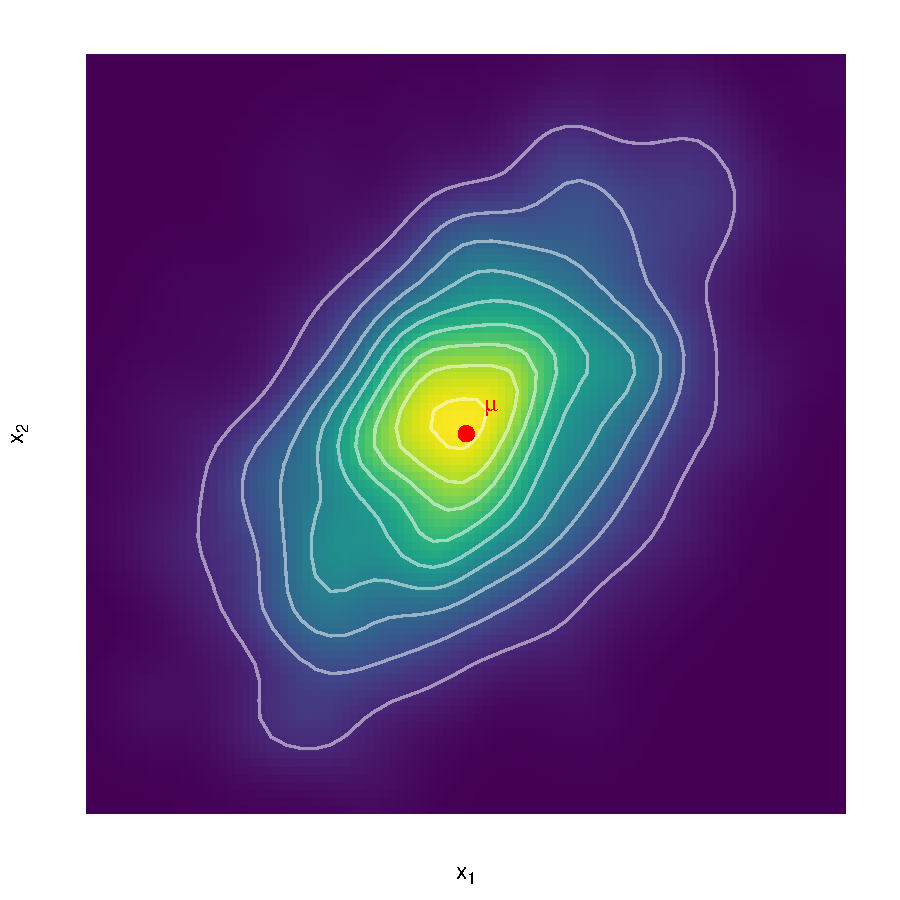
\includegraphics[width=1\textwidth]{multivariate_normal_2d.pdf} % Adjust the width and path as needed
    \caption{Multivariate Normal Distribution for Two Traits, $x_1$ and $x_2$, and where $u$ is the multivariate mean}
    \label{fig:Multivariate NOrmal 2D} % Label for referencing the figure
\end{figure}
\newpage

\tableofcontents
\begin{figure}[h] % "h" means the figure will appear here in the text
    \centering
    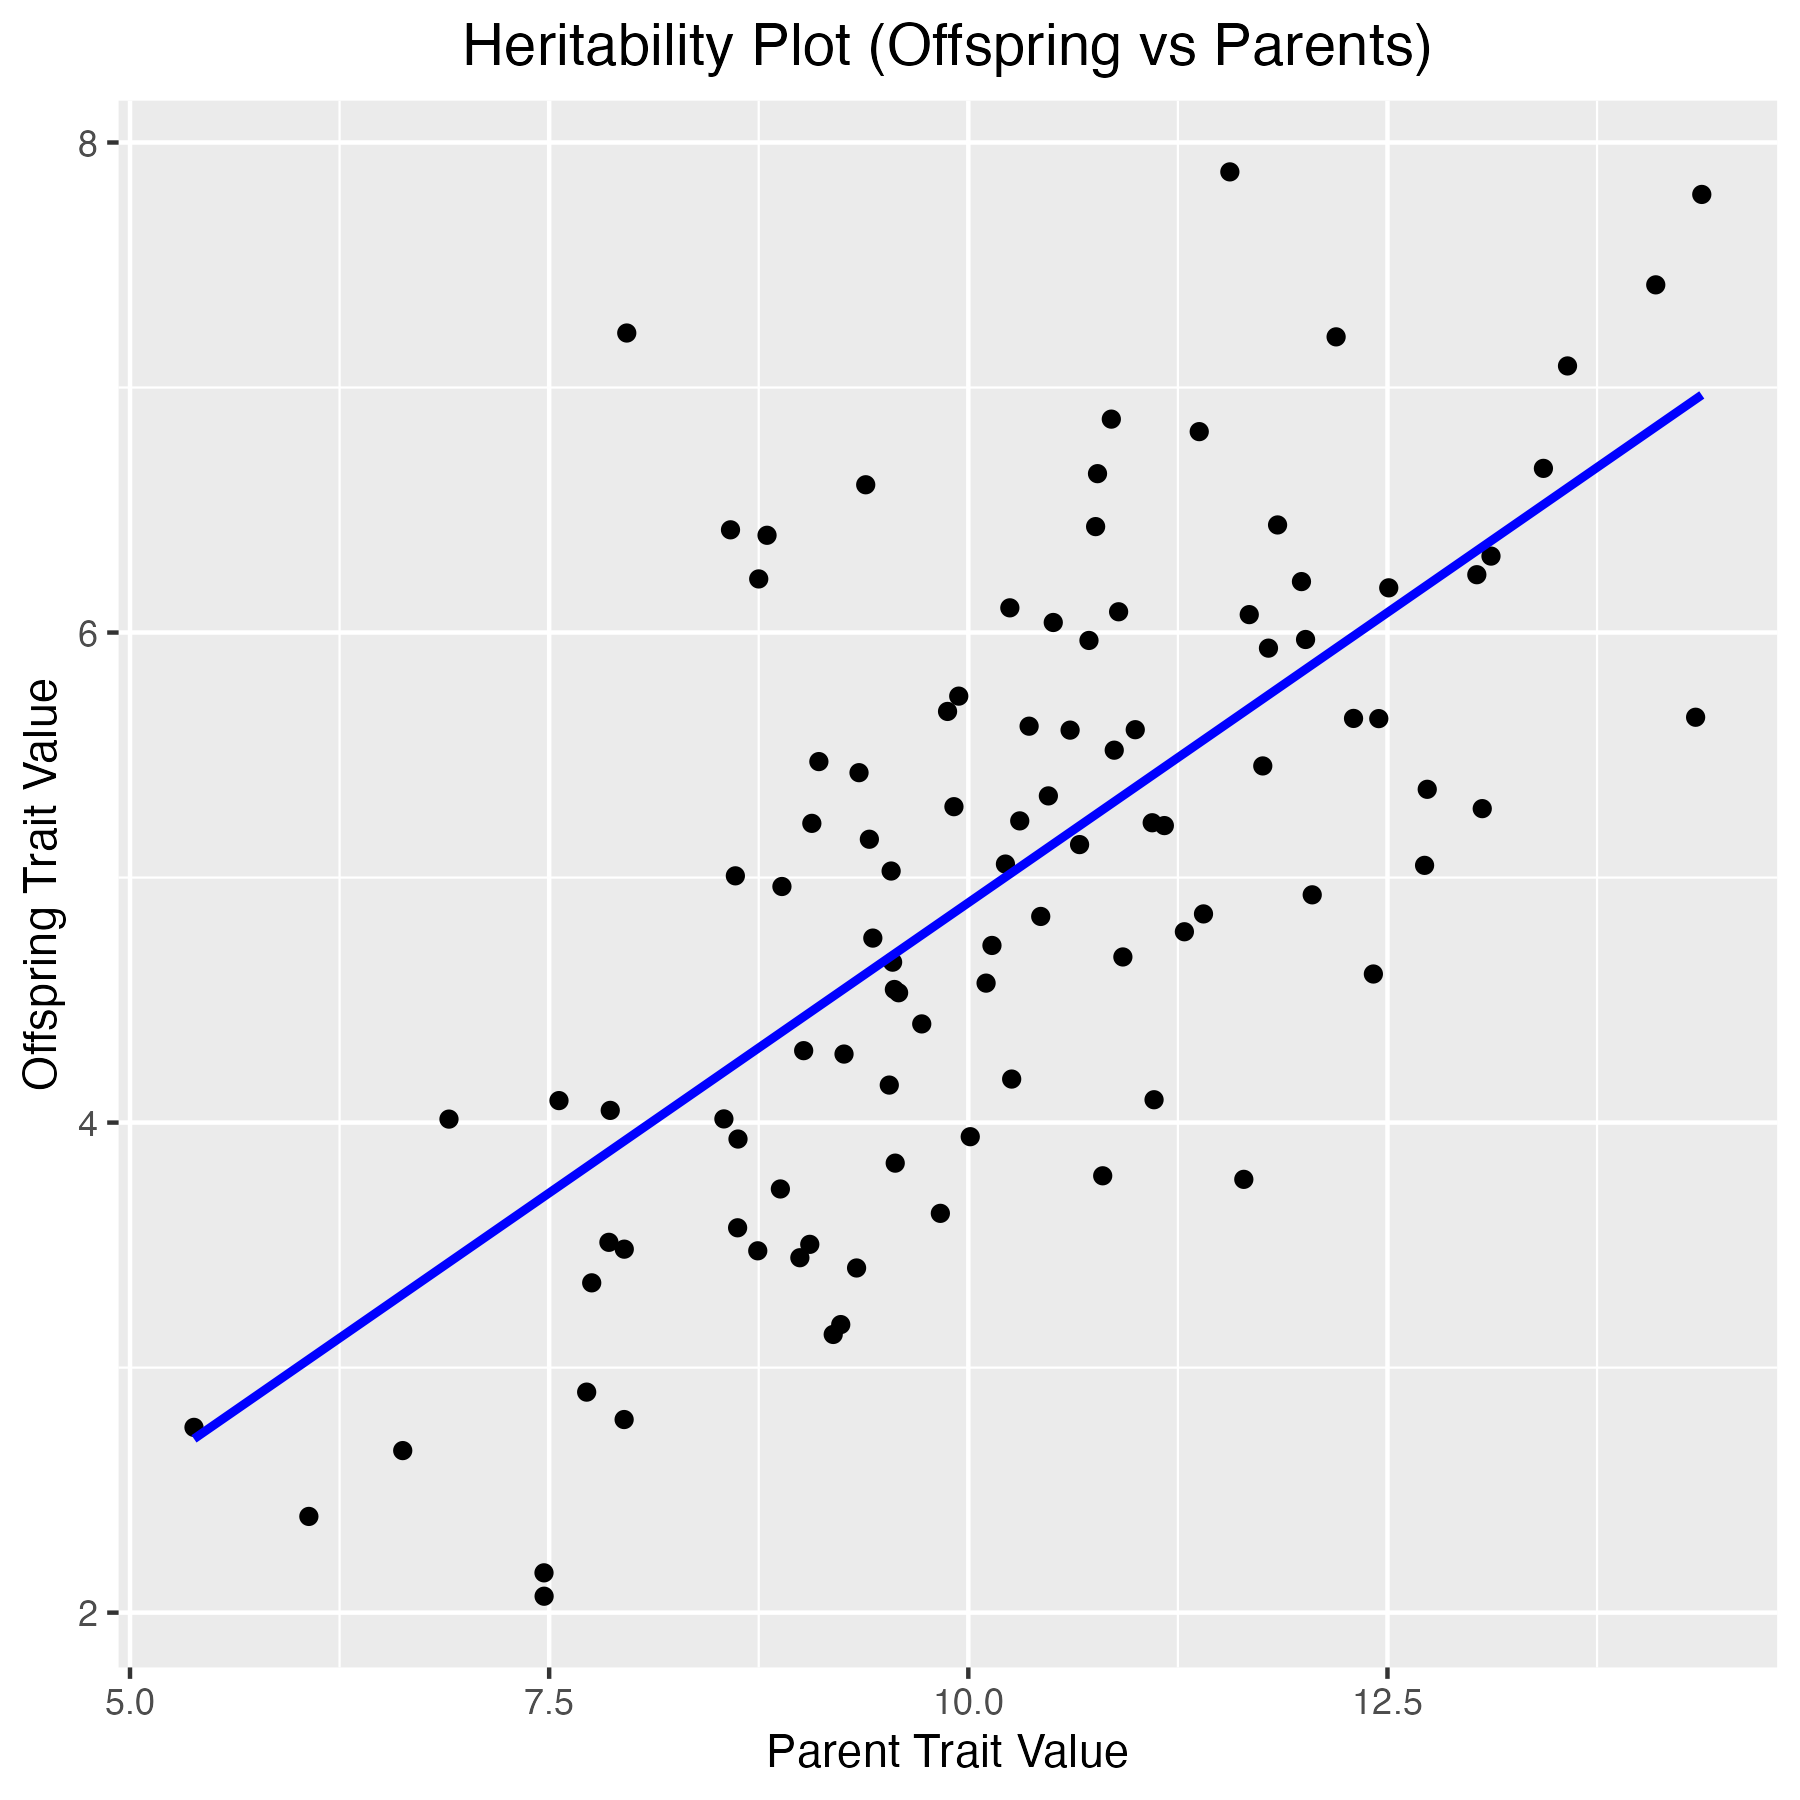
\includegraphics[width=0.8\textwidth]{heritability_plot.png} % Adjust the width and path as needed
    \caption{The slope of the line approximates the heritability of the trait}
    \label{fig:Heritability} % Label for referencing the figure
\end{figure}
\newpage

\begin{abstract}
This document explores linear algebra concepts and their applications in plant breeding and evolutionary genetics. It is designed to bridge the gap between mathematical theory and biological research. It shows how advanced statistical methods can enhance our understanding of genetic variation and its interaction with the environment. The document begins with an introduction to fundamental mathematical concepts, including vectors, matrices, and their operations. These foundational ideas are then extended to more complex statistical concepts such as likelihood and the multivariate normal distribution, which form the basis of modern quantitative genetics. A key focus is on the development and application of linear mixed models, particularly Best Linear Unbiased Prediction (BLUP) and its genomic counterpart, GBLUP. These statistical tools are explained in detail, from their mathematical derivation to their practical implementation in R, making the content accessible to both theoretically inclined researchers and empirical scientists.\\

The document also explores the role of the kinship matrix in accounting for genetic relationships, a concept that has improved both plant breeding and evolutionary studies. By incorporating this information, researchers can more accurately estimate genetic effects and predict breeding values as they examine variability in natural and agricultural systems. Throughout the text, the biological significance of these mathematical concepts is explained, with specific examples and interpretations provided for both plant breeding and evolutionary genetics contexts. This approach should help readers understand not just the 'how' but also the 'why' behind these methods. Advanced topics such as Bayesian approaches to mixed models are also covered, offering readers a glimpse into cutting-edge methodologies that are shaping the future of quantitative genetics. By the end of this document, readers will have gained a solid understanding of how linear algebra and statistical methods can be leveraged to gain deeper insights into genetic variation, adaptation, and the complex interplay between genes and environment. This knowledge is crucial for anyone involved in modern plant breeding programs or studying evolutionary processes in natural populations.
\end{abstract}

\section{Introduction}
This document explores the application of statistical and linear algebra concepts in plant breeding and evolutionary genetics, focusing on Best Linear Unbiased Estimates (BLUEs) and Best Linear Unbiased Predictions (BLUPs). We'll examine how these mathematical tools are used to understand plant traits, genetic adaptation, and evolutionary processes.

\section{Introduction to Basic Statistics and Genetics}

This section is aimed at readers with little to no background in statistics or genetics, providing an intuitive foundation before tackling more advanced concepts in the document.

\subsection{What is Statistics?}

Statistics is the science of collecting, analysing, and interpreting data. In biology, we use statistics to make sense of the variation we observe in nature. For example, we may ask: "Is the average height of plants in one population significantly different from another?"

\subsubsection{Descriptive Statistics}

Descriptive statistics summarise data. Key concepts include:

\begin{itemize}
    \item \textbf{Mean (Average)}: The central value of a data set, calculated as the sum of all values divided by the number of observations.
    \item \textbf{Variance}: A measure of how much the values in a data set vary. If variance is high, the values are spread out; if low, they are close to the mean.
    \item \textbf{Standard Deviation}: The square root of variance, providing an understanding of spread in the same units as the original data.
\end{itemize}

\begin{keyconceptbox}[Mean and Standard Deviation Example]
Suppose we measure the heights of 5 plants in centimetres: 10, 12, 9, 11, and 13 cm. The mean height is:
\[
\text{Mean} = \frac{10 + 12 + 9 + 11 + 13}{5} = 11 \, \text{cm}
\]
The standard deviation helps us understand the variation in plant height.
\end{keyconceptbox}

\begin{interpretation}[Biological Interpretation: Understanding Variation in Populations]
In biology, variance and standard deviation are crucial for understanding how traits like plant height vary across populations. For example, if the variance in plant height is high within a population, it might indicate diverse genetic backgrounds or varying environmental conditions. Standard deviation helps researchers gauge how far individual measurements (e.g., heights) are from the population mean, which is essential for predicting evolutionary potential or making breeding decisions.
\end{interpretation}

\subsubsection{Inferential Statistics}

Inferential statistics allow us to make conclusions about a population based on a sample. Key methods include:

\begin{itemize}
    \item \textbf{Hypothesis Testing}: A method to determine whether observed data differs from a theoretical expectation. For example, we can test if the average height of plants in two populations is significantly different.
    \item \textbf{Confidence Intervals}: These provide a range within which we are confident the true population parameter lies, given the observed data.
\end{itemize}

\begin{example}[Hypothesis Testing: Plant Heights]
We compare the heights of plants in two populations. We assume no difference in height between the two populations (the null hypothesis). By using a t-test, we determine whether observed differences are likely due to random variation or reflect true differences.
\end{example}

\subsection{Introduction to Genetics}

Genetics is the study of how traits are inherited. In evolutionary genetics, we are particularly interested in how genetic variation leads to differences in traits that can affect survival and reproduction.

\subsubsection{Genes and Alleles}

\begin{keyconceptbox}[Genetic Terminology]
\textbf{Gene}: A unit of heredity made of DNA that codes for a protein or functional RNA.\\
\textbf{Allele}: Different forms of a gene that can exist at a specific locus. For example, alleles may cause variation in flower colour.
\end{keyconceptbox}

\subsubsection{Genotype and Phenotype}

The genotype is the genetic makeup of an organism, while the phenotype is the observable traits. These traits are influenced by both the genotype and environmental factors.

\begin{interpretation}[Genotype-Phenotype Relationship]
Not all genetic variation leads to observable differences in the phenotype. The relationship between genes and traits is often complex, as genes may interact with each other and the environment to shape traits.
\end{interpretation}

\subsection{Why Statistics and Genetics Matter Together}

In evolutionary biology and genetics, statistical methods help us quantify how genes contribute to phenotypic traits and how traits evolve over time. For example, we may want to understand how much of the variation in plant height is due to genetic differences versus environmental factors. This understanding is key to predicting how populations will respond to natural selection.

\begin{keyconceptbox}[Application of Statistics in Genetics]
One of the major goals of genetics is to estimate how heritable traits are—i.e., the proportion of phenotypic variation due to genetic factors. Statistical models, such as linear regression and mixed models, help us quantify these relationships.
\end{keyconceptbox}

\section{Experimental Design in Plant Breeding and Evolutionary Genetics}

In both plant breeding and evolutionary genetics, well-thought-out experimental design is crucial for obtaining valid, reproducible results. Experimental design refers to how treatments, controls, and randomisation are structured within a study. Below, we cover key concepts and common types of experimental designs, with examples relevant to both disciplines.

\subsection{Key Concepts in Experimental Design}

\begin{keyconceptbox}[Key Concepts]
\begin{itemize}
    \item \textbf{Replication}: Repeating an experiment under the same conditions to estimate the variability and ensure reliability of the results.
    \item \textbf{Randomisation}: Assigning treatments or genotypes randomly to experimental units to avoid bias.
    \item \textbf{Blocking}: Grouping experimental units with similar characteristics to reduce variation within treatments.
    \item \textbf{Control Treatments}: Including a treatment group that does not receive the experimental intervention to provide a baseline for comparison.
    \item \textbf{Factorial Design}: Investigating the effect of multiple factors simultaneously, where each factor has multiple levels.
\end{itemize}
\end{keyconceptbox}

\subsection{Completely Randomised Design (CRD)}

In a Completely Randomised Design, treatments are assigned randomly to experimental units. This design is often used when environmental conditions are relatively uniform, as it does not control for variation in space or time.

\begin{example}[CRD in Plant Breeding]
Suppose we are testing the effect of different fertiliser types on plant height. We randomly assign fertiliser treatments to 100 plants in a glasshouse. Because the conditions (e.g., light, temperature) are controlled and uniform, the CRD is appropriate.
\end{example}

\subsection{Randomised Complete Block Design (RCBD)}

In a Randomised Complete Block Design, experimental units are divided into blocks that are expected to be more similar to each other. Treatments are then randomly assigned within each block. This design reduces variability between treatments by controlling for block-level factors (e.g., soil fertility in a field experiment).

\begin{example}[RCBD in Evolutionary Genetics]
In a study on plant response to drought, we may divide plants into blocks based on their position in the field (e.g., different rows that receive varying amounts of sunlight). Within each block, we randomly assign genotypes to control for spatial variation across the field.
\end{example}

\subsection{Factorial Design}

A factorial design is used when multiple factors are of interest. Each factor has two or more levels, and the design allows researchers to test for both the individual effects of each factor and any interactions between them.

\begin{example}[Factorial Design in Plant Breeding]
Consider a breeding experiment that tests the effect of both fertiliser type and watering regime on plant growth. The two factors (fertiliser and watering) have two levels each (e.g., organic vs. chemical fertiliser, high vs. low watering). A factorial design allows us to test not only the main effects of fertiliser and watering but also how they interact.
\end{example}

\subsection{Split-Plot Design}

In a split-plot design, one factor is applied to large experimental units (plots), while another factor is applied to sub-units (split plots) within each plot. This is particularly useful in field experiments where one factor (e.g., a genetic treatment) is harder to change or randomise than another (e.g., environmental conditions).

\begin{example}[Split-Plot Design in Evolutionary Genetics]
Imagine testing the response of different plant genotypes to both fertiliser type and temperature. Fertiliser treatments can be applied to large plots, while genotypes are assigned within sub-plots, allowing the study of genotype-environment interactions.
\end{example}

\subsection{Nested Design}

A nested design is used when treatments are nested within each other, such as when smaller units (e.g., individual plants) are grouped within larger units (e.g., plots or populations). This design is ideal for hierarchical experiments where variation exists at multiple levels.

\begin{example}[Nested Design in Evolutionary Studies]
In an evolutionary genetics study, we might test how different populations of a plant species respond to environmental stress. Each population might have several genotypes, and each genotype is tested in multiple replicates. The nested design allows us to assess variability both within and between populations.
\end{example}

\subsection{Crossed Design}

A crossed design is used when the same experimental units are subjected to multiple treatments. This allows for the assessment of interactions between treatments across the same subjects or experimental units.

\begin{example}[Crossed Design in Plant Breeding]
If we want to assess how different genotypes respond to varying fertiliser types across different environmental conditions, we could apply each treatment combination to the same set of genotypes across several environments. This allows for testing both main effects and genotype-environment interactions.
\end{example}

\subsection{Importance of Randomisation and Replication}

Randomisation ensures that treatment effects are not confounded by systematic biases, while replication increases the reliability of the results. Both are essential for obtaining valid and generalisable results.

\begin{keyconceptbox}[Best Practices in Experimental Design]
\begin{itemize}
    \item Always randomise the assignment of treatments to avoid bias.
    \item Include enough replicates to estimate variability and ensure robustness.
    \item Choose an appropriate design that accounts for potential sources of variation (e.g., block designs to control for spatial variation in field studies).
\end{itemize}
\end{keyconceptbox}

\section{Conclusion}

Experimental design is a fundamental aspect of research in plant breeding and evolutionary genetics. Choosing the appropriate design ensures that results are reliable and interpretable, and it maximises the ability to detect true biological effects. By carefully considering replication, randomisation, and the choice of design, researchers can draw meaningful conclusions about the genetic and environmental factors that shape phenotypic traits.

\section{Mathematical Background}

\subsection{Introduction: The Importance of Mathematics in BLUP and Quantitative Genetics}

Best Linear Unbiased Prediction (BLUP) is a powerful statistical technique widely used in plant breeding, animal breeding, and evolutionary genetics. At its core, BLUP is a sophisticated mathematical method that relies heavily on concepts from linear algebra and statistics. 

Understanding these mathematical foundations is crucial for several reasons:

\begin{enumerate}
    \item Model Formulation: BLUP models are expressed using matrices and vectors. The ability to interpret and manipulate these structures is essential for setting up appropriate models for different breeding scenarios.

    \item Computational Efficiency: Many of the operations in BLUP, such as matrix inversion, can be computationally intensive. A solid grasp of matrix properties and operations allows for the development and use of more efficient algorithms.

    \item Interpretation of Results: The output of BLUP analyses often comes in the form of vectors and matrices. Proper interpretation of these results requires an understanding of what these mathematical objects represent in a biological context.

    \item Model Assumptions: BLUP relies on certain assumptions about the statistical properties of the data, many of which are expressed in mathematical terms. Understanding these assumptions is critical for proper application and interpretation of BLUP.

    \item Extension and Innovation: As genetics and breeding face new challenges, such as incorporating genomic data or dealing with non-additive genetic effects, the ability to extend and modify BLUP methods often requires a deep understanding of its mathematical underpinnings.
\end{enumerate}

In the following subsections, we will explore key mathematical concepts that form the foundation of BLUP and other quantitative genetics methods. These include basic matrix operations, statistical concepts like expectation and variance, and specific matrix properties that are particularly relevant to BLUP calculations. By mastering these concepts, you will be better equipped to understand, apply, and potentially extend BLUP methodologies in your work.

\subsection{Linear Algebra Concepts}

\subsubsection{Vectors and Matrices}

Vectors and matrices are fundamental to the mathematical formulation of BLUP and many other quantitative genetics methods. In this document, we will denote vectors with bold lowercase letters (e.g., $\mathbf{y}$) and matrices with bold uppercase letters (e.g., $\mathbf{X}$).

\begin{keyconceptbox}
A vector is an ordered collection of numbers, while a matrix is a rectangular array of numbers. In the context of BLUP, vectors often represent observations or effects, while matrices typically represent design structures or relationships between individuals.
\end{keyconceptbox}

\textbf{Example:}\\
Vector: $$\mathbf{y} = \begin{pmatrix} 2 \\ 1 \end{pmatrix}$$
This vector might represent phenotypic measurements (e.g., plant height) for two individuals.

Matrix: $$\mathbf{X} = \begin{pmatrix} 1 & 2 \\ 3 & 4 \end{pmatrix}$$
This matrix could represent a design matrix where rows correspond to observations and columns to different effects (e.g., treatments or environments).

In quantitative genetics, we often work with several types of matrices:
\begin{itemize}
    \item Design matrices ($\mathbf{X}$ and $\mathbf{Z}$) that link observations to fixed and random effects
    \item Variance-covariance matrices that describe the genetic and residual variation
    \item Relationship matrices (e.g., kinship matrices) that capture genetic similarities between individuals
\end{itemize}

\begin{example}
In a plant breeding experiment, we might represent the yield of different varieties across multiple locations as a matrix:

\[
\mathbf{Y} = \begin{pmatrix}
    5.2 & 4.8 & 5.5 \\
    6.1 & 5.9 & 6.3 \\
    4.9 & 5.1 & 5.0
\end{pmatrix}
\]

Here, each row represents a plant variety, and each column represents a location. The entry $Y_{ij}$ is the yield (in tons per hectare) of the $i$-th variety at the $j$-th location.
\end{example}

\begin{interpretation}
This matrix representation allows breeders to quickly compare variety performance across different environments. For instance, we can see that the second variety (row 2) generally outperforms the others across all locations.
\end{interpretation}


\subsubsection{Matrix Operations}

Understanding matrix operations is crucial for working with the equations involved in BLUP and other quantitative genetics methods. We'll cover three key operations: multiplication, transpose, and inverse.

\paragraph{Matrix Multiplication}: Matrix multiplication is a fundamental operation in linear algebra and is central to many calculations in BLUP. 

\begin{greenbox}
The product of two matrices $\mathbf{A}$ and $\mathbf{B}$ is defined element-wise as:

$$(\mathbf{AB})_{ij} = \sum_k A_{ik}B_{kj}$$

\end{greenbox}

It's important to note that matrix multiplication is only defined when the number of columns in the first matrix equals the number of rows in the second matrix.

\textbf{Example:}\\
Let $$\mathbf{A} = \begin{pmatrix} 1 & 2 \\ 3 & 4 \end{pmatrix}$$ and $$\mathbf{B} = \begin{pmatrix} 5 & 6 \\ 7 & 8 \end{pmatrix}$$

The product $\mathbf{AB}$ is calculated as follows:

\begin{align*}
(\mathbf{AB})_{11} &= (1 \times 5) + (2 \times 7) = 5 + 14 = 19 \\
(\mathbf{AB})_{12} &= (1 \times 6) + (2 \times 8) = 6 + 16 = 22 \\
(\mathbf{AB})_{21} &= (3 \times 5) + (4 \times 7) = 15 + 28 = 43 \\
(\mathbf{AB})_{22} &= (3 \times 6) + (4 \times 8) = 18 + 32 = 50
\end{align*}

Therefore, $$\mathbf{AB} = \begin{pmatrix} 19 & 22 \\ 43 & 50 \end{pmatrix}$$

In BLUP, matrix multiplication is used extensively, for example, when calculating the variance-covariance matrix of observations or when applying the mixed model equations.

\begin{example}
Consider a simple genetic model where we want to predict phenotypic values based on genotypic effects. Let's say we have three loci with additive effects:

\[
\mathbf{G} = \begin{pmatrix}
    1 & 0 & 2 \\
    2 & 1 & 1 \\
    0 & 2 & 1
\end{pmatrix}, \quad
\mathbf{a} = \begin{pmatrix}
    0.5 \\
    0.3 \\
    0.2
\end{pmatrix}
\]

Here, $\mathbf{G}$ represents the genotype matrix for three individuals (rows) at three loci (columns), and $\mathbf{a}$ represents the additive effect of each locus.

The predicted phenotypic values are given by $\mathbf{p} = \mathbf{G}\mathbf{a}$:

\[
\mathbf{p} = \begin{pmatrix}
    1 & 0 & 2 \\
    2 & 1 & 1 \\
    0 & 2 & 1
\end{pmatrix}
\begin{pmatrix}
    0.5 \\
    0.3 \\
    0.2
\end{pmatrix}
= \begin{pmatrix}
    0.9 \\
    1.4 \\
    0.7
\end{pmatrix}
\]
\end{example}

\begin{interpretation}
This matrix multiplication allows us to efficiently calculate predicted phenotypic values for multiple individuals based on their genotypes and the estimated effects of each locus. The result shows that the second individual is expected to have the highest phenotypic value, which could inform selection decisions in a breeding program.
\end{interpretation}

\paragraph{Matrix Transpose}:
The transpose operation is crucial in many BLUP calculations, particularly when dealing with design matrices.

\begin{greenbox}
The transpose of a matrix is obtained by interchanging its rows and columns. For a matrix $\mathbf{A}$, its transpose $\mathbf{A}'$ is defined as:

$(\mathbf{A}')_{ij} = A_{ji}$
\end{greenbox}

\textbf{Example:}
Given $$\mathbf{A} = \begin{pmatrix} 1 & 2 \\ 3 & 4 \end{pmatrix}$$

Its transpose is:

$$\mathbf{A}' = \begin{pmatrix} 1 & 3 \\ 2 & 4 \end{pmatrix}$$

In BLUP, we often use transposes when forming cross-products (e.g., $\mathbf{X'X}$) or when dealing with variance-covariance structures.

\paragraph{Matrix Inverse}:
Matrix inversion is a critical operation in solving the mixed model equations in BLUP.

\begin{greenbox}
The inverse of a square matrix $\mathbf{A}$, denoted as $\mathbf{A}^{-1}$, is a matrix that, when multiplied with $\mathbf{A}$, yields the identity matrix:

$$\mathbf{A}\mathbf{A}^{-1} = \mathbf{A}^{-1}\mathbf{A} = \mathbf{I}$$
\end{greenbox}

\textbf{Example:}
For $$\mathbf{A} = \begin{pmatrix} 2 & 1 \\ 1 & 3 \end{pmatrix}$$

The inverse is calculated as follows:

1. Calculate the determinant: $$det(\mathbf{A}) = (2 \times 3) - (1 \times 1) = 5$$

2. Find the adjugate matrix: $$adj(\mathbf{A}) = \begin{pmatrix} 3 & -1 \\ -1 & 2 \end{pmatrix}$$

3. $$\mathbf{A}^{-1} = \frac{1}{det(\mathbf{A})} \times adj(\mathbf{A}) = \frac{1}{5} \times \begin{pmatrix} 3 & -1 \\ -1 & 2 \end{pmatrix}$$

Therefore, $$\mathbf{A}^{-1} = \begin{pmatrix} 3/5 & -1/5 \\ -1/5 & 2/5 \end{pmatrix}$$

In BLUP, matrix inversion is crucial for solving the mixed model equations and for calculating various components of the model.

\begin{figure}[h] % "h" means the figure will appear here in the text
    \centering
    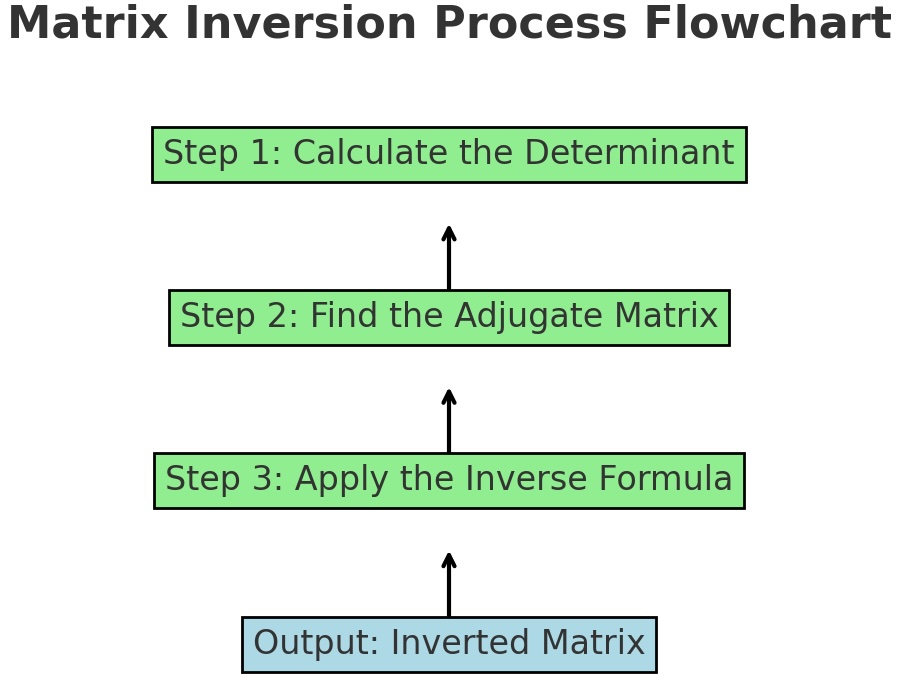
\includegraphics[width=0.6\textwidth]{matrixInv_FC.jpg} % Adjust the width and path as needed
    \label{fig:Inverse of a Matrix} % Label for referencing the figure
\end{figure}

\subsection{Statistical Concepts}

\subsubsection{Expectation and Variance}

Expectation and variance are fundamental concepts in probability theory and statistics that play a crucial role in the development of BLUP methodology.

\paragraph{Expectation}:

The expectation of a random variable $X$, denoted as $E(X)$, is its average or mean value over many repetitions. 

\begin{greenbox}
For a discrete random variable, the expectation of a random variable is calculated as:

$$E(X) = \sum_i x_i P(X = x_i)$$

where $x_i$ are the possible values of $X$ and $P(X = x_i)$ is the probability of $X$ taking the value $x_i$.
\end{greenbox}

In the context of BLUP, we often work with random vectors. 

\begin{greenbox}
    
The expectation of a random vector $\mathbf{X}$ is defined as:
$$E(\mathbf{X}) = [E(X_1), E(X_2), ..., E(X_n)]'$$
\end{greenbox}

\textbf{Example:}
Let $\mathbf{X}$ be a random vector representing the breeding values of two traits in a population:
$$\mathbf{X} = [X_1, X_2]$$
where $X_1$ and $X_2$ are the breeding values for trait 1 and trait 2 respectively. 

If we assume that the population mean breeding value for each trait is 0 (which is often done in quantitative genetics), then:

$$E(\mathbf{X}) = [E(X_1), E(X_2)] = [0, 0]$$ 

This concept is crucial in BLUP as we often work with breeding values and other genetic effects that are assumed to have an expectation of zero.

\paragraph{Variance and Covariance}

\leavevmode\vspace{1pt} % Inserts a smaller, fixed space (6pt)

In BLUP, variance and covariance matrices play a crucial role in describing the genetic and residual variability in the population.

\begin{greenbox}
    The variance of a random variable $X$, denoted as $Var(X)$ or $\sigma^2_X$, measures its spread or dispersion. It's defined as:

$$Var(X) = E[(X - E(X))^2]$$

For a random vector $\mathbf{X}$, the variance-covariance matrix is defined as:

$$Var(\mathbf{X}) = E[(\mathbf{X} - E(\mathbf{X}))(\mathbf{X} - E(\mathbf{X}))']$$

The covariance between two random variables $X$ and $Y$ is defined as:

$$Cov(X,Y) = E[(X - E(X))(Y - E(Y))]$$
\end{greenbox}

\textbf{Example:}
Continuing with our two-trait example, let's say we have estimated the genetic variance for trait 1 as 0.5, for trait 2 as 0.7, and the genetic covariance between them as 0.2. The genetic variance-covariance matrix would be:

$$Var(\mathbf{X}) = \begin{pmatrix} 0.5 & 0.2 \\ 0.2 & 0.7 \end{pmatrix}$$

This matrix is crucial in multi-trait BLUP models, as it describes the genetic relationship between the traits.

\begin{example}
In a population genetics study of a tree species, we measure the height of adult trees in two different populations:

Population A: $\{18, 20, 22, 19, 21\}$ meters
Population B: $\{15, 17, 16, 18, 14\}$ meters

The expectations (means) are:
$E(A) = 20$ meters
$E(B) = 16$ meters

The variances are:
$Var(A) = 2$ m²
$Var(B) = 2.5$ m²
\end{example}

\begin{interpretation}
The expectation tells us about the average height in each population, suggesting that trees in Population A tend to be taller. The variance gives us information about the spread of heights within each population. Despite the difference in mean height, the similar variances indicate that both populations have comparable levels of height variability. This could suggest that while environmental factors might be causing the difference in mean height (e.g., better growing conditions in the habitat of Population A), the underlying genetic variability for height might be similar in both populations.
\end{interpretation}

\subsection{Likelihood and Multivariate Normal Distribution}

The concepts of likelihood and the multivariate normal distribution are fundamental to the statistical framework of BLUP and many other quantitative genetics methods.

\subsubsection{Likelihood}

The likelihood function is a key concept in statistical inference. It represents the probability of observing the data given a particular set of parameter values.

\begin{keyconceptbox}
For a set of observations $\mathbf{y}$ and parameters $\boldsymbol{\theta}$, the likelihood function is denoted as $L(\boldsymbol{\theta}|\mathbf{y})$.
\end{keyconceptbox}

In the context of BLUP and mixed models, we often work with the log-likelihood, which has more convenient mathematical properties:

$$\log L(\boldsymbol{\theta}|\mathbf{y}) = -\frac{1}{2} \log |\mathbf{V}| - \frac{1}{2} (\mathbf{y} - \mathbf{X\beta})' \mathbf{V}^{-1} (\mathbf{y} - \mathbf{X\beta}) + constant$$

Where:
\begin{itemize}
    \item $\mathbf{V}$ is the variance-covariance matrix of $\mathbf{y}$
    \item $\mathbf{X}$ is the design matrix for fixed effects
    \item $\boldsymbol{\beta}$ is the vector of fixed effects
\end{itemize}

\begin{interpretation}[Biological Interpretation: Likelihood in Trait Inheritance]
In evolutionary genetics, likelihood is used to assess how well different genetic models explain the inheritance of traits. For example, when studying a trait like drought tolerance, researchers might compare different models with varying assumptions about the number of genes involved. The model with the highest likelihood is the one that most likely explains the observed pattern of trait inheritance in a population.
\end{interpretation}

\subsubsection{Multivariate Normal Distribution}

The multivariate normal distribution is a generalization of the one-dimensional normal distribution to higher dimensions. It's a key assumption in many quantitative genetics models, including BLUP.

\begin{keyconceptbox}[Probability Density Function]
For a k-dimensional random vector $\mathbf{x}$, the probability density function of the multivariate normal distribution is:

\[
f(\mathbf{x}) = (2\pi)^{-k/2} |\boldsymbol{\Sigma}|^{-1/2} \exp\left(-\frac{1}{2} (\mathbf{x} - \boldsymbol{\mu})' \boldsymbol{\Sigma}^{-1} (\mathbf{x} - \boldsymbol{\mu})\right)
\]
\end{keyconceptbox}

Where:
\begin{itemize}
    \item $\mathbf{x}$ is a k-dimensional random vector
    \item $\boldsymbol{\mu}$ is the k-dimensional mean vector
    \item $\boldsymbol{\Sigma}$ is the k × k covariance matrix
    \item $|\boldsymbol{\Sigma}|$ is the determinant of $\boldsymbol{\Sigma}$
    \item $(\mathbf{x} - \boldsymbol{\mu})'$ is the transpose of $(\mathbf{x} - \boldsymbol{\mu})$
\end{itemize}

\begin{figure}[htbp]
  \centering
  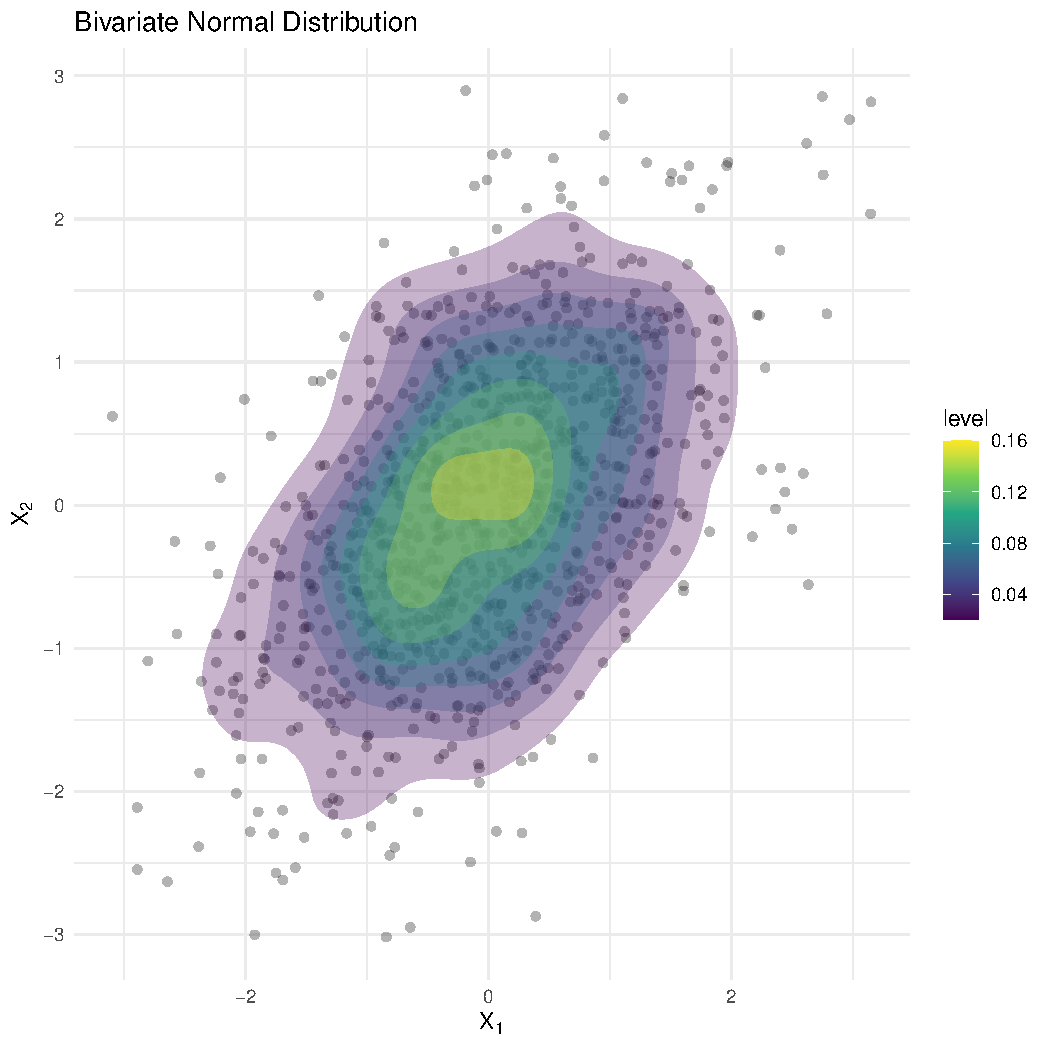
\includegraphics[width=1\textwidth]{multivariate_normal.pdf}
  \caption{Visualization of a bivariate normal distribution}
  \label{fig:multivariate_normal}
\end{figure}

In BLUP, we often assume that the random effects (e.g., breeding values) follow a multivariate normal distribution. This assumption allows us to derive the best  linear unbiased predictor.

\begin{keyconceptbox}[Application in BLUP]
In the context of BLUP, we often assume:

\begin{itemize}
    \item The vector of random effects $\mathbf{u}$ follows a multivariate normal distribution: 
    $\mathbf{u} \sim MVN(0, \mathbf{G})$, where $\mathbf{G}$ is the genetic variance-covariance matrix.
    \item The vector of residuals $\mathbf{e}$ also follows a multivariate normal distribution: 
    $\mathbf{e} \sim MVN(0, \mathbf{R})$, where $\mathbf{R}$ is the residual variance-covariance matrix.
\end{itemize}

These assumptions allow us to derive the mixed model equations and obtain BLUPs.
\end{keyconceptbox}

The multivariate normal distribution has several properties that make it particularly useful in quantitative genetics:

1. Linear combinations of multivariate normal variables are also normally distributed. This property is crucial when dealing with genetic effects that are sums of many small contributions (as in the infinitesimal model).

2. The conditional distributions are also multivariate normal. This property is used in deriving the equations for BLUP.

3. Maximum likelihood estimation for the multivariate normal distribution has a closed-form solution, which simplifies the estimation of variance components.

\begin{example}
In a quantitative trait locus (QTL) mapping study for drought tolerance in maize, we might model the joint distribution of two related traits: root length (RL) and yield under drought stress (YD). Assuming these traits follow a bivariate normal distribution:

\[
\begin{pmatrix} RL \\ YD \end{pmatrix} \sim N\left(\begin{pmatrix} \mu_{RL} \\ \mu_{YD} \end{pmatrix}, \begin{pmatrix} \sigma^2_{RL} & \sigma_{RL,YD} \\ \sigma_{RL,YD} & \sigma^2_{YD} \end{pmatrix}\right)
\]

Where:
$\mu_{RL} = 30$ cm (mean root length)
$\mu_{YD} = 5$ t/ha (mean yield under drought)
$\sigma^2_{RL} = 25$ cm² (variance of root length)
$\sigma^2_{YD} = 1$ (t/ha)² (variance of yield under drought)
$\sigma_{RL,YD} = 3$ cm·t/ha (covariance between root length and yield)
\end{example}

\begin{interpretation}
This multivariate normal model captures not only the individual variation in root length and yield under drought but also their relationship. The positive covariance suggests that plants with longer roots tend to have higher yields under drought conditions. This information can be valuable for breeders aiming to improve drought tolerance, as selecting for increased root length might indirectly improve yield performance under water-limited conditions.
\end{interpretation}

\subsection{Matrix Properties Relevant to BLUP}

Several matrix properties are particularly important in the context of BLUP and other quantitative genetics methods. Understanding these properties is crucial for ensuring the validity of BLUP calculations and for interpreting the results correctly.

\begin{keyconceptbox}

A symmetric matrix $\mathbf{A}$ is positive definite if $\mathbf{x}'\mathbf{A}\mathbf{x} > 0$ for all non-zero vectors $\mathbf{x}$. 
\end{keyconceptbox}

This property is crucial in BLUP for several reasons:

\begin{enumerate}
    \item Variance-Covariance Matrices: In BLUP, the genetic and residual variance-covariance matrices must be positive definite. This ensures that the variances are positive and the matrix can be inverted.
    \item Mixed Model Equations: The coefficient matrix of the mixed model equations in BLUP must be positive definite to ensure a unique solution.
    \item Numerical Stability: Positive definiteness helps ensure numerical stability in computations, particularly when inverting matrices.
\end{enumerate}

\textbf{Example:}
The matrix $$\mathbf{A} = \begin{pmatrix} 2 & 1 \\ 1 & 2 \end{pmatrix}$$ is positive definite.
We can verify this by checking if all eigenvalues are positive:
Eigenvalues of $\mathbf{A}$ are $\lambda_1 = 3$ and $\lambda_2 = 1$, which are both positive.

\subsubsection{Singularity and Rank}

A matrix is singular if its determinant is zero, meaning it doesn't have a unique inverse. The rank of a matrix is the number of linearly independent rows or columns. These concepts are important in BLUP for:

\begin{itemize}
\item Mixed Model Equations: If the coefficient matrix is singular, there isn't a unique solution to the BLUP equations.
\item Variance Component Estimation: Singularity can cause problems in estimating variance components, a crucial step in BLUP.
\item Genomic BLUP: In genomic BLUP, the genomic relationship matrix may be singular if there are more markers than individuals, requiring special handling.
\end{itemize}

\textbf{Example:}
The matrix $$\mathbf{B} = \begin{pmatrix} 1 & 2 \\ 2 & 4 \end{pmatrix}$$ is singular.
Its determinant is $1(4) - 2(2) = 0$, and its rank is 1.

In genomic BLUP, we might encounter this issue when we have more genetic markers than individuals in our dataset. In such cases, specialized techniques like ridge regression BLUP (rrBLUP) or principal component regression can be used to handle the singularity.

\subsubsection{Orthogonality}

Two vectors are orthogonal if their dot product is zero. In matrix terms, columns (or rows) of a matrix are orthogonal if $\mathbf{x}'\mathbf{y} = 0$ for any two distinct columns (or rows) $\mathbf{x}$ and $\mathbf{y}$. Orthogonality is relevant to BLUP in:

\begin{itemize}
\item Design Matrices: Orthogonal design matrices can simplify calculations and interpretation in BLUP.
\item Random Effects: In some BLUP applications, it's assumed that different random effects are orthogonal to each other.
\end{itemize}

\textbf{Example:}
The columns of the matrix $$\mathbf{C} = \begin{pmatrix} 1 & 0 & 1 \\ 1 & 1 & -1 \\ 1 & -1 & 0 \end{pmatrix}$$ are orthogonal to each other.

In the context of BLUP, orthogonality can be particularly useful in experimental design. For instance, in a plant breeding trial, if we can design our experiment such that the effects of different factors (e.g., genotype, environment, treatment) are orthogonal, it can simplify our analysis and improve the precision of our estimates.

\subsection{The Role of These Concepts in BLUP}

Now that we've covered these mathematical concepts, let's briefly discuss how they come together in BLUP:

1. Vectors and Matrices: BLUP uses vectors to represent observations, breeding values, and other effects. Matrices are used to represent the structure of the data and the relationships between individuals.

2. Matrix Operations: The BLUP equations involve multiple matrix multiplications and inversions. Understanding these operations is crucial for implementing and interpreting BLUP.

3. Expectation and Variance: These concepts are fundamental to understanding the statistical properties of BLUP. The expectation of BLUP is unbiased, and its variance is minimized among all linear unbiased predictors.

4. Multivariate Normal Distribution: This distribution is a key assumption in deriving BLUP. It allows us to model complex patterns of genetic and environmental variation.

5. Likelihood: The BLUP equations can be derived by maximizing the likelihood (or equivalently, the log-likelihood) of the data under the mixed model.

6. Matrix Properties: Positive definiteness ensures that our variance-covariance matrices are valid and that our equations have unique solutions. Understanding singularity and rank helps us handle situations with limited data or high-dimensional genetic information.

\begin{biologicalinsightbox}
While these mathematical concepts might seem abstract, they allow us to model complex biological phenomena:

\begin{itemize}
    \item The multivariate normal distribution models the idea that many small genetic effects combine to influence quantitative traits.
    \item Variance-covariance matrices capture the genetic relationships between individuals and traits.
    \item Matrix operations allow us to efficiently handle large datasets, crucial in the era of genomic selection.
    \item The properties of BLUP (best, linear, unbiased) make it a powerful tool for predicting genetic merit in breeding programs.
\end{itemize}
\end{biologicalinsightbox}

Understanding these mathematical foundations not only allows us to use BLUP effectively but also enables us to extend and adapt these methods as we face new challenges in quantitative genetics and breeding.

\section{The Kinship Matrix and Natural Variability in Populations}
\subsection{Learning Objectives}
After this section, you'll be able to:
\begin{itemize}
    \item Explain how the kinship matrix captures the intricate web of genetic similarities in a population
    \item Visualize how genetic relationships influence trait variations in plants and animals
    \item Apply the concept of kinship to both carefully managed breeding programs and wild populations
    \item Appreciate how accounting for relatedness can dramatically improve our understanding of genetics
\end{itemize}

In the context of linear mixed models for plant breeding and evolutionary genetics, the kinship matrix plays a crucial role in accounting for natural variability within populations. This section explores the concept of the kinship matrix, its genetic basis, and its importance in statistical modeling of complex traits.

\begin{figure}[h]
    \centering
    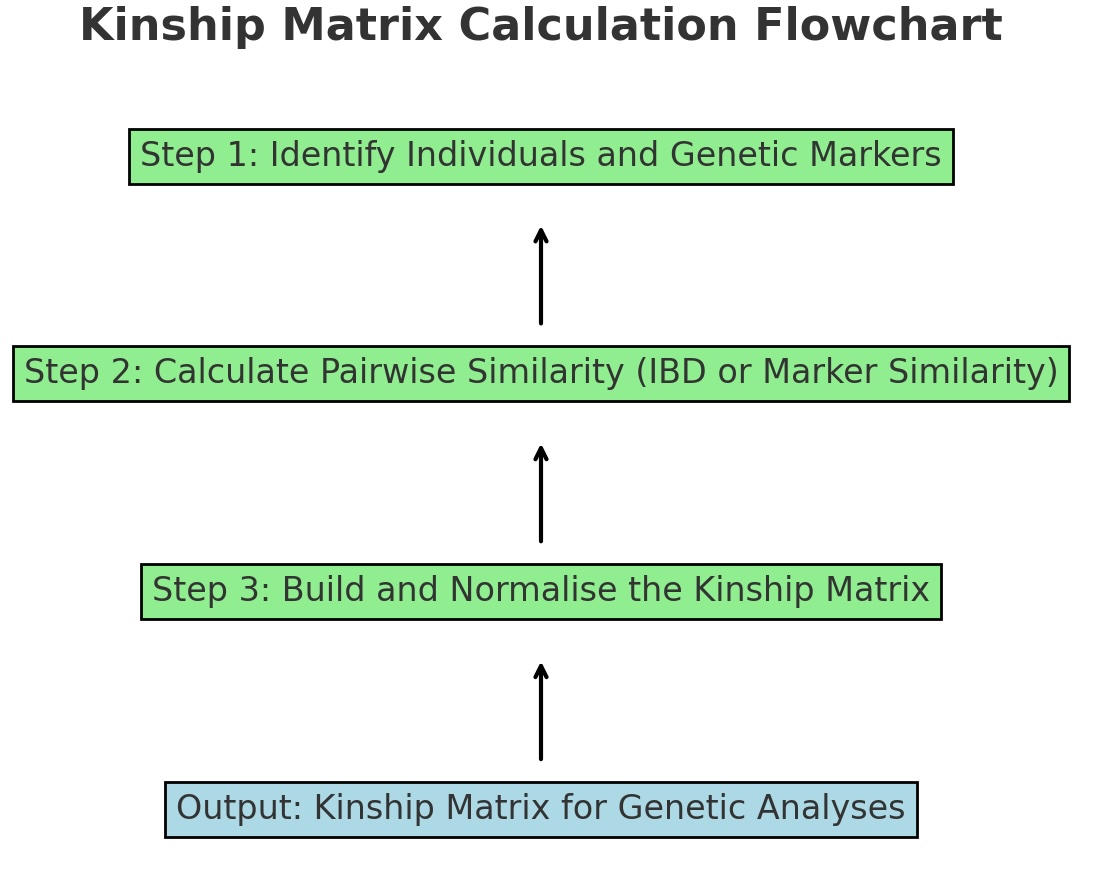
\includegraphics[width=0.6\textwidth]{kinshipMatrix_FC.jpg} % Example image
    \label{fig:Kinship Matrix Calculation}
\end{figure}
\subsection{Understanding the Kinship Matrix}

The kinship matrix, also known as the relatedness matrix, is a fundamental tool in quantitative genetics that represents the degree of genetic similarity between individuals in a population. It is based on the principle that related individuals share more genetic material than unrelated individuals and are therefore likely to be more similar in their traits.

\begin{keyconceptbox}
    
The kinship matrix quantifies the expected genetic similarity between all pairs of individuals in a population, allowing us to model the covariance structure of genetic effects.
\end{keyconceptbox}

At its core, the kinship matrix is built on the concept of identity by descent (IBD). Alleles that are identical copies of an ancestral allele are said to be identical by descent. The kinship coefficient between two individuals, which forms an element of the kinship matrix, essentially represents the probability that a randomly chosen allele from each individual at a given locus is identical by descent.

\subsection{Genetic Basis and Natural Variability}

The power of the kinship matrix in accounting for natural variability stems from its connection to fundamental genetic principles. In most quantitative traits, a large portion of genetic variance is additive, meaning that the effects of alleles at different loci combine additively to influence the trait. This additive genetic variance is precisely what the kinship matrix helps us capture in our models.

When we incorporate the kinship matrix into a linear mixed model, we're essentially modeling the covariance structure of the random genetic effects. This structure reflects the biological reality that more closely related individuals are expected to have more similar genetic values. By doing so, we can partition the total phenotypic variance into genetic and environmental components, allowing us to account for the portion of natural variability that is due to genetic factors.

\begin{biologicalinsightbox}
    
The kinship matrix allows us to connect statistical models with biological reality, reflecting the shared ancestry and genetic similarity that underlies phenotypic variation in populations.
\end{biologicalinsightbox}

\subsection{Mathematical Representation in Mixed Models}

In the framework of linear mixed models, we typically assume that the random genetic effects (u) follow a multivariate normal distribution:

\[
\mathbf{u} \sim MVN(0, \sigma^2_u\mathbf{K})
\]

Where $\sigma^2_u$ is the genetic variance and $\mathbf{K}$ is the kinship matrix. This formulation allows the model to account for the expected genetic similarity between individuals when estimating genetic effects and other model parameters.

\subsection{Implications for Plant Breeding and Evolutionary Genetics}

The incorporation of the kinship matrix into our models has profound implications for both plant breeding and evolutionary genetics studies. In plant breeding, it allows for more accurate estimation of breeding values and prediction of cross performance. For evolutionary geneticists, it provides a powerful tool for understanding the genetic basis of adaptation and the distribution of genetic variation within and between populations.

\begin{biologicalinsightbox}[Practical Impact]
    By accounting for genetic relationships, we can achieve improved accuracy in estimating both fixed effects (e.g., treatment effects) and random effects (e.g., breeding values), reduce bias in our estimates, and increase the statistical power to detect significant effects.
\end{biologicalinsightbox}

Moreover, the kinship matrix approach is incredibly flexible. It can handle a wide range of relationship structures, from simple pedigrees to complex populations with many distantly related individuals. This is particularly valuable in modern breeding programs and evolutionary studies, where we often deal with large, complex populations.

\subsection{Advanced Applications: Genomic Prediction}

In the era of high-throughput genotyping, the concept of the kinship matrix has been extended to genomic relationship matrices derived from dense genetic markers. This has enhanced breeding programs by allowing for accurate prediction of genetic values even for individuals without phenotypic data, a technique known as genomic selection.

\begin{figure}[htbp]
  \centering
  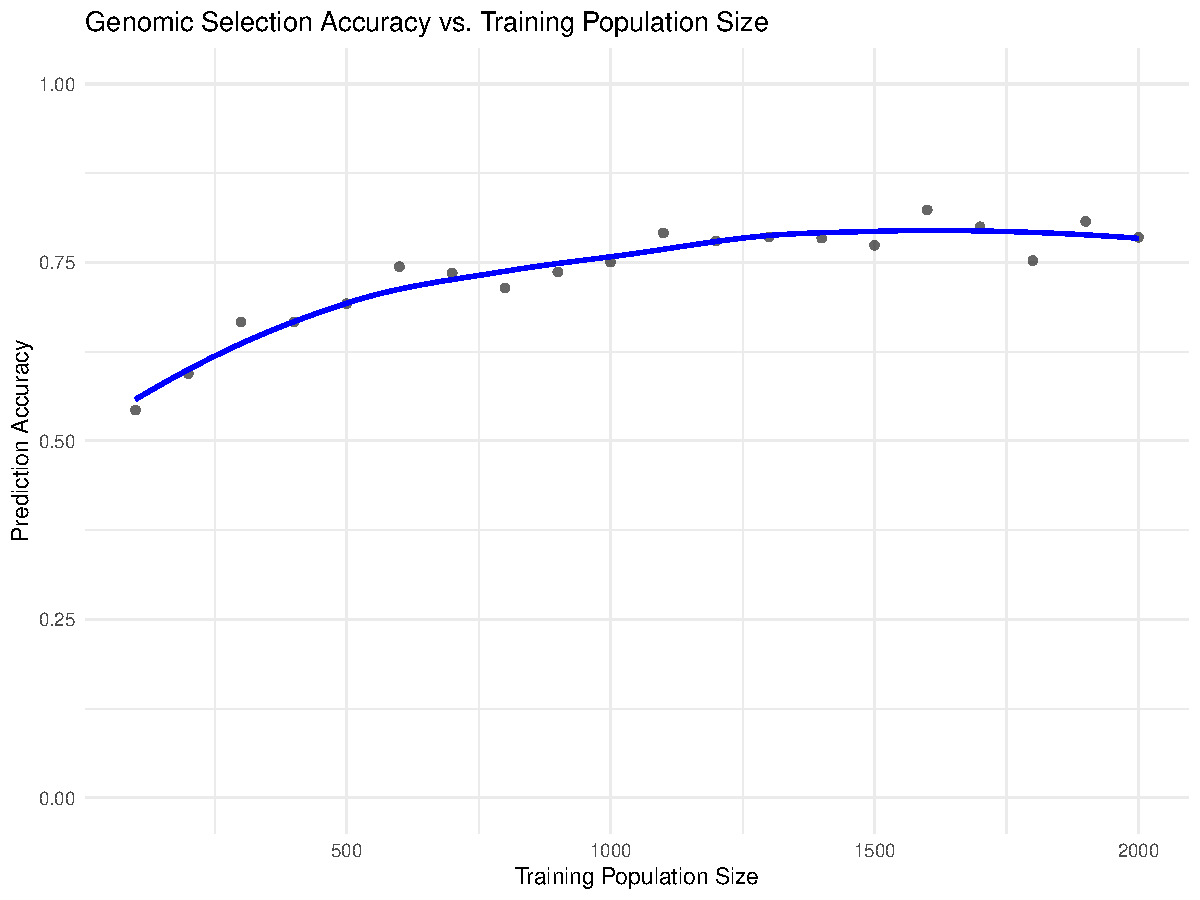
\includegraphics[width=0.8\textwidth]{gs_accuracy.pdf}
  \caption{Relationship between genomic selection accuracy and training population size}
  \label{fig:gs_accuracy}
\end{figure}

\subsection{Summary and Relevance}

The table below summarises the key aspects of the kinship matrix and its relevance to plant breeding and evolutionary genetics:

\begin{table}[h]
\centering
\begin{tabular}{|p{0.3\textwidth}|p{0.3\textwidth}|p{0.3\textwidth}|}
\hline
\textbf{Concept} & \textbf{Relevance to Plant Breeding} & \textbf{Relevance to Evolutionary Genetics} \\
\hline
Genetic Similarity & Improves accuracy of breeding value estimates & Helps understand genetic structure of populations \\
\hline
Variance Partitioning & Allows estimation of heritability and genetic correlations & Facilitates study of genetic basis of adaptation \\
\hline
Population Structure & Accounts for family relationships in breeding programs & Models complex evolutionary histories \\
\hline
Genomic Prediction & Enables efficient genomic selection & Predicts evolutionary potential of populations \\
\hline
\end{tabular}
\caption{Relevance of Kinship Matrix Concepts in Plant Breeding and Evolutionary Genetics}
\label{tab:kinship_relevance}
\end{table}

\begin{figure}[h]
    \centering
    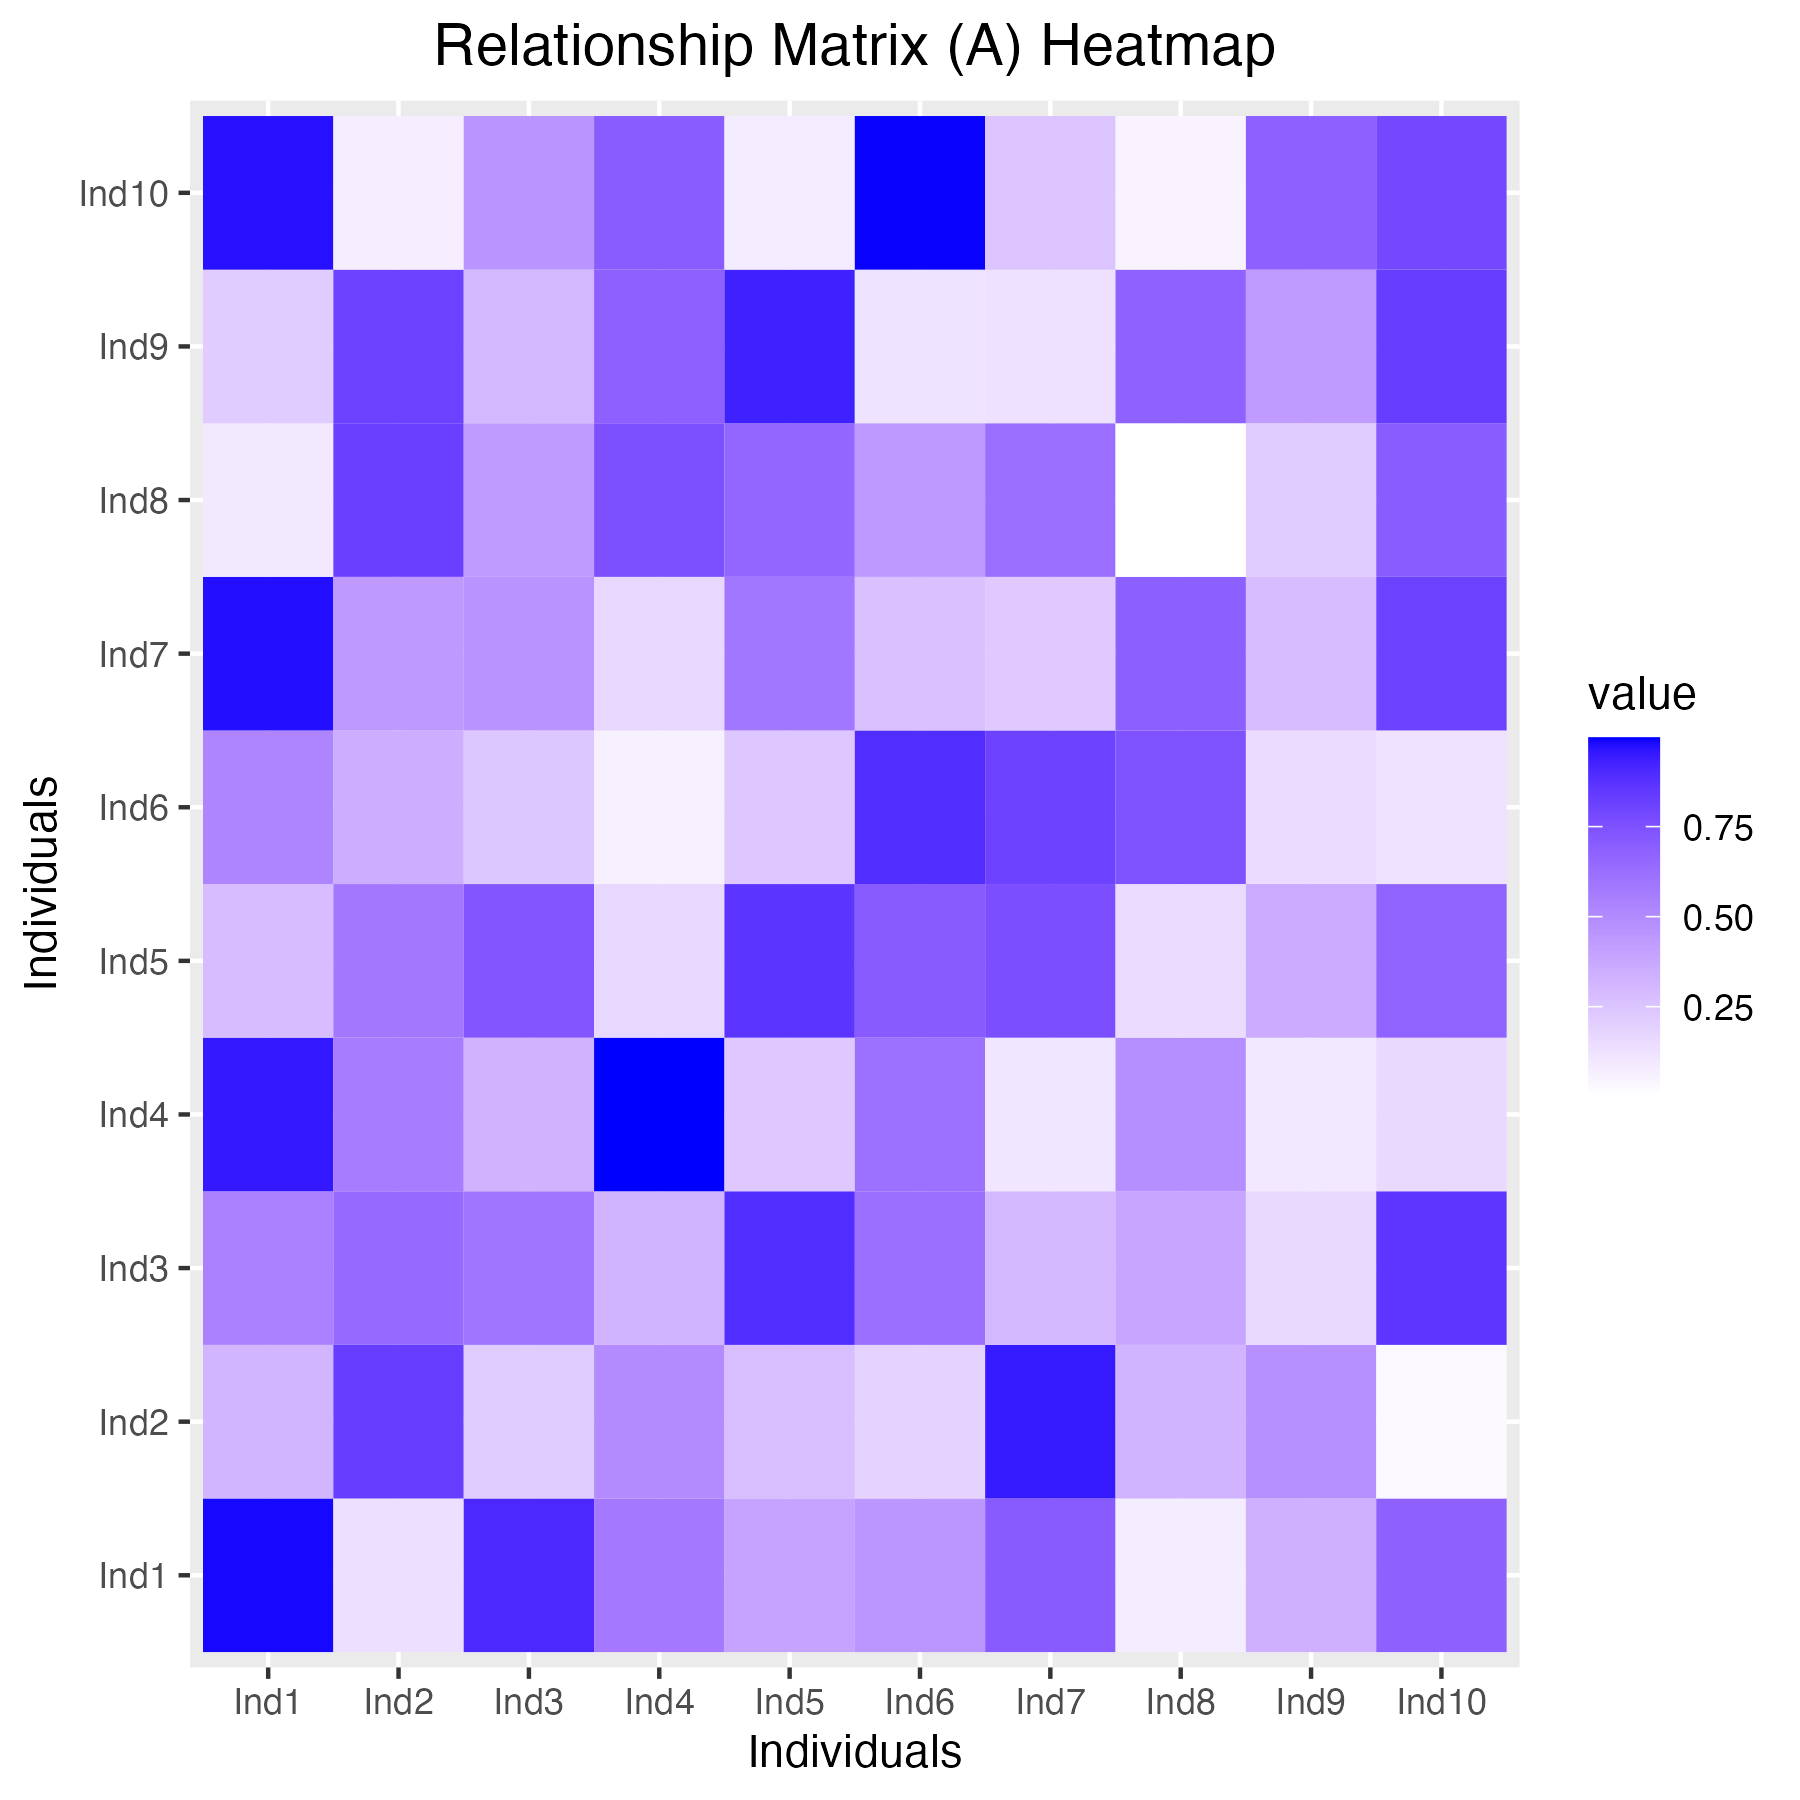
\includegraphics[width=0.8\textwidth]{relationship_matrix.png} % Example image
    \caption{Heatmap of the relationship matrix (A) illustrating genetic relatedness among individuals. Darker shades indicate stronger genetic relationships}
    \label{fig:Relationship Matrix}
\end{figure}


In conclusion, the kinship matrix is a powerful tool for accounting for natural genetic variability in populations. By incorporating information about genetic relationships, we can build more accurate and biologically meaningful models of quantitative traits. This is particularly important in fields like plant breeding and evolutionary genetics, where understanding and utilizing genetic variation is crucial for progress. As we continue to explore complex genetic architectures and develop more sophisticated breeding and analysis techniques, the kinship matrix will undoubtedly remain a cornerstone of quantitative genetic analysis.

\begin{example}
Consider a pedigree of three generations in a wheat breeding program:

\begin{tikzpicture}[level distance=1cm, sibling distance=3cm]
\node {P}
    child {node {F1}}
    child {node {F1}};
\node at (0,-2) {F2};
\end{tikzpicture}

The corresponding kinship matrix might look like:

\[
\mathbf{K} = \begin{pmatrix}
    1   & 0   & 0.5 & 0.5 & 0.25 \\
    0   & 1   & 0.5 & 0.5 & 0.25 \\
    0.5 & 0.5 & 1   & 0.5 & 0.5  \\
    0.5 & 0.5 & 0.5 & 1   & 0.5  \\
    0.25& 0.25& 0.5 & 0.5 & 1
\end{pmatrix}
\]

Where rows and columns represent: P1, P2, F1-1, F1-2, F2, respectively.
\end{example}

\begin{interpretation}
This kinship matrix quantifies the genetic relationships in our breeding population. The diagonal elements are 1, representing an individual's relationship to itself. Off-diagonal elements represent the proportion of shared genetic material between individuals. For instance, the 0.5 between P1 and F1-1 indicates that a parent shares, on average, half its genetic material with its offspring. This matrix is crucial in mixed model analyses, allowing us to account for genetic similarities when estimating breeding values or heritability of traits.
\end{interpretation}


\section{The Linear Mixed Model in Plant Breeding and Evolutionary Genetics}

\subsection{Basic Equation}

The linear mixed model in matrix notation is given by:

\begin{equation}
    \mathbf{y} = \mathbf{Xb} + \mathbf{Zu} + \mathbf{e}
\end{equation}

Where:
\begin{itemize}
    \item $\mathbf{y}$ is the vector of observations (e.g., plant phenotypic measurements)
    \item $\mathbf{b}$ is the vector of fixed effects
    \item $\mathbf{u}$ is the vector of random effects
    \item $\mathbf{e}$ is the vector of random residuals
    \item $\mathbf{X}$ and $\mathbf{Z}$ are design matrices
\end{itemize}

\begin{biologicalinsightbox}
    
In plant breeding, $\mathbf{y}$ could represent a vector of yield measurements for different crop varieties. The fixed effects $\mathbf{b}$ might include factors like location, year, and fertilizer treatment. The random effects $\mathbf{u}$ could represent the genetic values of individual plant lines or varieties.

In evolutionary genetics, $\mathbf{y}$ might represent fitness-related traits in natural populations. Fixed effects could include environmental factors, while random effects might represent individual genetic effects or population-specific adaptations.
\end{biologicalinsightbox}

\subsection{Design Matrices}

The design matrices $\mathbf{X}$ and $\mathbf{Z}$ connect the observations to the fixed and random effects, respectively.

\begin{biologicalinsightbox}
    In a plant breeding trial, $\mathbf{X}$ might have columns for each level of location, year, and treatment, with entries of 0 or 1 indicating which effects apply to each observation. $\mathbf{Z}$ would typically have one column per plant line or variety.

For evolutionary studies, $\mathbf{X}$ might represent environmental gradients or distinct habitats, while $\mathbf{Z}$ could represent individual genotypes or population memberships.
\end{biologicalinsightbox}

\section{Distributional Assumptions}

For the random effects and residuals, we have the following distributional assumptions:

\begin{align}
    \mathbf{u} &\sim MVN(0, \sigma^2_g\mathbf{K}) \\
    \mathbf{e} &\sim MVN(0, \sigma^2_e\mathbf{I})
\end{align}

Where:
\begin{itemize}
    \item $MVN$ denotes the multivariate normal distribution
    \item $\mathbf{K}$ is the kinship matrix (for plant breeding) or population covariance matrix (for evolutionary genetics)
    \item $\sigma^2_g$ is the genetic variance
    \item $\sigma^2_e$ is the residual variance
    \item $\mathbf{I}$ is the identity matrix
\end{itemize}

\begin{biologicalinsightbox}

In plant breeding, the kinship matrix $\mathbf{K}$ captures the genetic relationships between different plant lines or varieties. This could be based on pedigree information or molecular markers.

In evolutionary genetics, $\mathbf{K}$ might represent the genetic covariance structure among populations, reflecting shared evolutionary history or gene flow. The assumption of a multivariate normal distribution for $\mathbf{u}$ aligns with the infinitesimal model of quantitative genetics, which assumes many genes of small effect contribute to trait variation.
\end{biologicalinsightbox}

\section{Derivation and Explanation of Henderson's Mixed Model Equations (MME)}

Henderson's Mixed Model Equations (MME) are fundamental to the application of linear mixed models in plant breeding and evolutionary genetics. This section will derive these equations step by step, explaining both the mathematical concepts and their biological interpretations.

\begin{figure}[h]
    \centering
    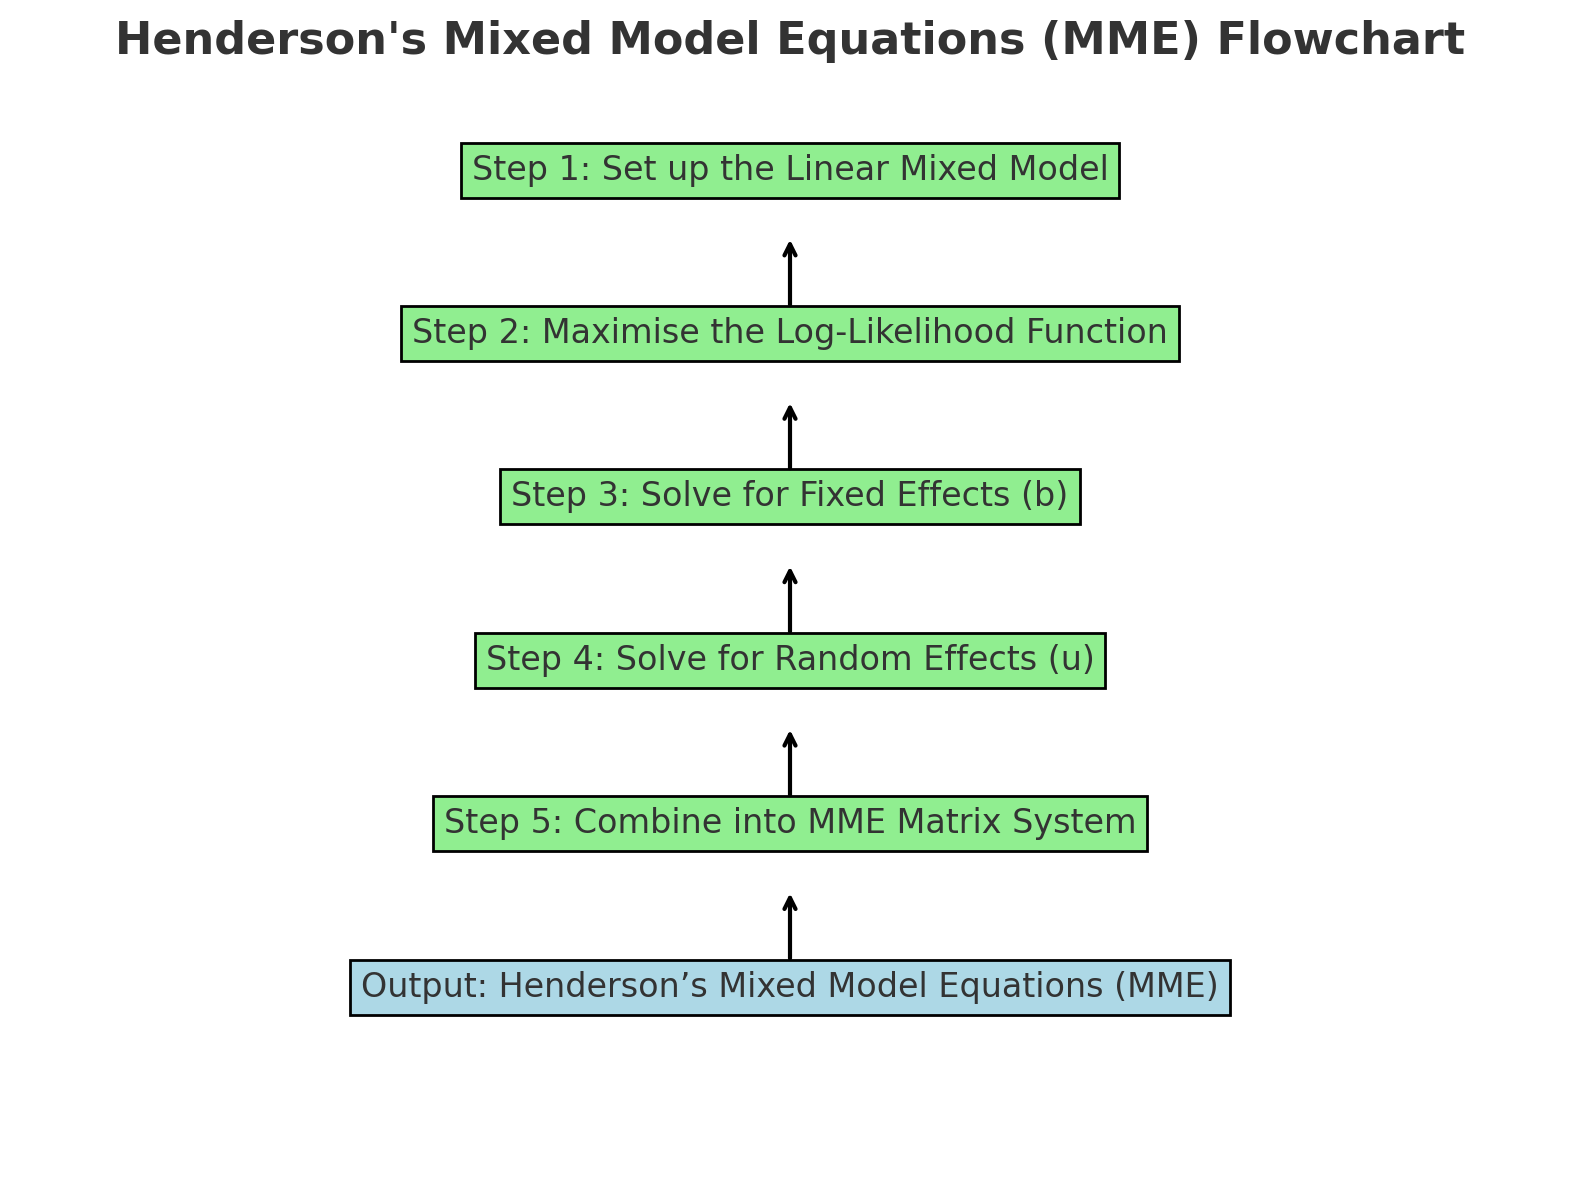
\includegraphics[width=1\textwidth]{hendersonMME_FC.png}
    \caption{Henderson's Mixed Model Equations (MME) flowchart outlining the steps from setting up the linear mixed model to solving the matrix system.}
    \label{fig:henderson-mme-flowchart}
\end{figure}


\subsection{Introduction to MME}

\begin{keyconceptbox}
    
Henderson's MME provide a framework for simultaneously estimating fixed effects and predicting random effects in a linear mixed model.
\end{keyconceptbox}

In the context of plant breeding and evolutionary genetics, MME allow us to:
\begin{itemize}
    \item Estimate environmental effects (fixed effects)
    \item Predict genetic values or breeding values (random effects)
    \item Account for complex genetic relationships between individuals
\end{itemize}

\subsection{The Linear Mixed Model}

Recall our linear mixed model:

\[
\mathbf{y} = \mathbf{Xb} + \mathbf{Zu} + \mathbf{e}
\]

Where:
\begin{itemize}
    \item $\mathbf{y}$ is the vector of observations (e.g., plant heights, yield)
    \item $\mathbf{X}$ is the design matrix for fixed effects
    \item $\mathbf{b}$ is the vector of fixed effects (e.g., environmental factors, treatments)
    \item $\mathbf{Z}$ is the design matrix for random effects
    \item $\mathbf{u}$ is the vector of random effects (e.g., genetic values)
    \item $\mathbf{e}$ is the vector of residuals
\end{itemize}

\begin{interpretation}[Biological Interpretation: Fixed Effects in Environmental Studies]
Fixed effects capture consistent relationships between environmental variables (such as temperature or rainfall) and phenotypic traits (such as plant height or flowering time). In plant breeding or evolutionary studies, fixed effects help quantify how much of the variation in a trait is due to measurable environmental factors. For example, a strong fixed effect of temperature might suggest that certain populations are highly responsive to temperature changes, indicating potential for rapid adaptation to climate change.
\end{interpretation}


\subsection{Formulating the Log-Likelihood}

We start by writing the log-likelihood function for the model:

\[
L(\mathbf{b}, \mathbf{u}) = -\frac{1}{2} \log |\mathbf{V}| - \frac{1}{2} (\mathbf{y} - \mathbf{Xb} - \mathbf{Zu})' \mathbf{V}^{-1} (\mathbf{y} - \mathbf{Xb} - \mathbf{Zu})
\]

\begin{biologicalinsightbox}

The log-likelihood function measures how well our model explains the observed data. It balances model complexity with goodness of fit. In biological terms, we're asking: "How likely are we to observe these phenotypes given our assumptions about genetic and environmental effects?"
\end{biologicalinsightbox}

Where $\mathbf{V}$ is the variance-covariance matrix of $\mathbf{y}$:

\[
\mathbf{V} = \sigma^2_g\mathbf{ZKZ'} + \sigma^2_e\mathbf{I}
\]

Here, $\mathbf{K}$ is the kinship matrix, $\sigma^2_g$ is the genetic variance, and $\sigma^2_e$ is the residual variance.

\subsection{Deriving the MME}

We derive the MME by maximizing the log-likelihood with respect to both $\mathbf{b}$ and $\mathbf{u}$.

\subsubsection{Step 1: Maximizing with Respect to Fixed Effects ($\mathbf{b}$)}

We take the derivative of the log-likelihood with respect to $\mathbf{b}$ and set it to zero:

\[
\frac{\partial L(\mathbf{b}, \mathbf{u})}{\partial \mathbf{b}} = -\mathbf{X'} \mathbf{V}^{-1} (\mathbf{y} - \mathbf{Xb} - \mathbf{Zu}) = 0
\]

This simplifies to:

\[
\mathbf{X'} \mathbf{V}^{-1} \mathbf{y} = \mathbf{X'} \mathbf{V}^{-1} \mathbf{Xb} + \mathbf{X'} \mathbf{V}^{-1} \mathbf{Zu}
\]

\begin{biologicalinsightbox}[Biological Meaning]
This equation represents the best estimate of fixed effects (e.g., environmental factors) while accounting for the random genetic effects. It's like asking, "What are the true environmental effects after we've accounted for genetic variation?"
\end{biologicalinsightbox}

\subsubsection{Step 2: Maximizing with Respect to Random Effects ($\mathbf{u}$)}

Now we take the derivative with respect to $\mathbf{u}$:

\[
\frac{\partial L(\mathbf{b}, \mathbf{u})}{\partial \mathbf{u}} = -\mathbf{Z'} \mathbf{V}^{-1} (\mathbf{y} - \mathbf{Xb} - \mathbf{Zu}) + \sigma^2_g \mathbf{K}^{-1} \mathbf{u} = 0
\]

This simplifies to:

\[
\mathbf{Z'} \mathbf{V}^{-1} \mathbf{y} = \mathbf{Z'} \mathbf{V}^{-1} \mathbf{Xb} + \mathbf{Z'} \mathbf{V}^{-1} \mathbf{Zu} + \sigma^2_g \mathbf{K}^{-1} \mathbf{u}
\]

\begin{biologicalinsightbox}[Biological Meaning]

This equation gives us the best prediction of random genetic effects while accounting for fixed environmental effects. It's answering the question, "What are the true genetic values after we've accounted for known environmental factors?"
\end{biologicalinsightbox}

\subsubsection{Step 3: Combining the Equations}

We now have two equations that we can combine into a single matrix equation:

\[
\begin{bmatrix}
    \mathbf{X'} \mathbf{V}^{-1} \mathbf{X} & \mathbf{X'} \mathbf{V}^{-1} \mathbf{Z} \\
    \mathbf{Z'} \mathbf{V}^{-1} \mathbf{X} & \mathbf{Z'} \mathbf{V}^{-1} \mathbf{Z} + \sigma^2_g \mathbf{K}^{-1}
\end{bmatrix}
\begin{bmatrix}
    \mathbf{b} \\
    \mathbf{u}
\end{bmatrix}
=
\begin{bmatrix}
    \mathbf{X'} \mathbf{V}^{-1} \mathbf{y} \\
    \mathbf{Z'} \mathbf{V}^{-1} \mathbf{y}
\end{bmatrix}
\]

This system of equations is Henderson's Mixed Model Equations (MME).

\subsection{Understanding the Components of MME}

Let's break down each component of the MME:

\begin{itemize}
    \item $\mathbf{X'} \mathbf{V}^{-1} \mathbf{X}$: This term represents the information content of the fixed effects.
\end{itemize}
    \begin{tcolorbox}[colback=green!5!white,colframe=uqpurple!75!black,title=Biological Interpretation]
    This quantifies how much the environmental factors (fixed effects) contribute to explaining the observed variation in traits.
    \end{tcolorbox}

\begin{itemize}
    \item $\mathbf{X'} \mathbf{V}^{-1} \mathbf{Z}$ and $\mathbf{Z'} \mathbf{V}^{-1} \mathbf{X}$: These terms capture the relationship between fixed and random effects.
\end{itemize}
    \begin{tcolorbox}[colback=green!5!white,colframe=uqpurple!75!black,title=Biological Interpretation]
    These terms account for how environmental factors and genetic effects interact to influence the observed traits.
    \end{tcolorbox}

\begin{itemize}
    \item $\mathbf{Z'} \mathbf{V}^{-1} \mathbf{Z} + \sigma^2_g \mathbf{K}^{-1}$: This term relates to the random effects.
\end{itemize}
    \begin{tcolorbox}[colback=green!5!white,colframe=uqpurple!75!black,title=Biological Interpretation]
    This represents the genetic information content, including both the observed data ($\mathbf{Z'} \mathbf{V}^{-1} \mathbf{Z}$) and prior knowledge about genetic relationships ($\sigma^2_g \mathbf{K}^{-1}$).
    \end{tcolorbox}

\begin{itemize}
    \item $\mathbf{X'} \mathbf{V}^{-1} \mathbf{y}$ and $\mathbf{Z'} \mathbf{V}^{-1} \mathbf{y}$: These are the right-hand side terms.
\end{itemize}
    \begin{tcolorbox}[colback=green!5!white,colframe=uqpurple!75!black,title=Biological Interpretation]
    These terms represent how the observed data relates to the fixed environmental effects and random genetic effects, respectively.
    \end{tcolorbox}

\subsection{Solving Henderson's MME}

To solve Henderson's MME, we use standard matrix algebra techniques such as Gaussian elimination or Cholesky decomposition. The solution provides:

\begin{itemize}
    \item $\hat{\mathbf{b}}$: Best Linear Unbiased Estimates (BLUEs) of the fixed effects
    \item $\hat{\mathbf{u}}$: Best Linear Unbiased Predictions (BLUPs) of the random effects
\end{itemize}

\begin{biologicalinsightbox}[Significance in Plant Breeding and Evolutionary Genetics]

In plant breeding:
\begin{itemize}
    \item $\hat{\mathbf{b}}$ estimates environmental factors like location or treatment effects
    \item $\hat{\mathbf{u}}$ predicts genetic values for different plant lines or varieties
\end{itemize}

In evolutionary genetics:
\begin{itemize}
    \item $\hat{\mathbf{b}}$ might estimate environmental selection gradients
    \item $\hat{\mathbf{u}}$ could represent breeding values or population-specific deviations from the mean
\end{itemize}
\end{biologicalinsightbox}

\begin{interpretation}[Biological Interpretation: Predicting Breeding Values with BLUP]
BLUP is a powerful tool in plant breeding because it allows breeders to predict the genetic value of individual plants, even if they haven't been fully tested in field conditions. For instance, in a wheat breeding program, BLUP helps breeders estimate which plants carry the best genetic traits for yield or disease resistance, based on both their own performance and that of their relatives. This prediction allows breeders to select superior plants earlier in the breeding process.
\end{interpretation}


\subsection{Conclusion}

Henderson's MME provide a powerful framework for simultaneously estimating environmental effects and predicting genetic values in plant breeding and evolutionary genetics. By accounting for both fixed and random effects, as well as the genetic relationships between individuals, these equations allow for more accurate and biologically meaningful analyses of complex traits.

\subsection{Solving Henderson's MME}

After deriving Henderson's Mixed Model Equations, the next step is to solve them to obtain the Best Linear Unbiased Estimates (BLUEs) of fixed effects and Best Linear Unbiased Predictions (BLUPs) of random effects. Let's walk through this process step by step.

Recall the MME in matrix form:

\[
\begin{bmatrix}
    \mathbf{X'} \mathbf{V}^{-1} \mathbf{X} & \mathbf{X'} \mathbf{V}^{-1} \mathbf{Z} \\
    \mathbf{Z'} \mathbf{V}^{-1} \mathbf{X} & \mathbf{Z'} \mathbf{V}^{-1} \mathbf{Z} + \sigma^2_g \mathbf{K}^{-1}
\end{bmatrix}
\begin{bmatrix}
    \mathbf{b} \\
    \mathbf{u}
\end{bmatrix}
=
\begin{bmatrix}
    \mathbf{X'} \mathbf{V}^{-1} \mathbf{y} \\
    \mathbf{Z'} \mathbf{V}^{-1} \mathbf{y}
\end{bmatrix}
\]

We can represent this more compactly as:

\[
\mathbf{C} \begin{bmatrix} \mathbf{b} \\ \mathbf{u} \end{bmatrix} = \mathbf{r}
\]

Where $\mathbf{C}$ is the coefficient matrix and $\mathbf{r}$ is the right-hand side.

\subsubsection{Step 1: Matrix Inversion}

The first step in solving this system is to invert the coefficient matrix $\mathbf{C}$. In practice, this is often done using numerical methods such as Cholesky decomposition or LU factorization, especially for large systems. However, for illustration, we'll show the direct inversion:

\[
\begin{bmatrix} \hat{\mathbf{b}} \\ \hat{\mathbf{u}} \end{bmatrix} = \mathbf{C}^{-1} \mathbf{r}
\]

\begin{biologicalinsightbox}[Biological Interpretation]

This inversion step is essentially weighing all the information we have - from both the fixed environmental effects and the random genetic effects - to come up with our best estimates and predictions.
\end{biologicalinsightbox}

\subsubsection{Step 2: Calculating BLUEs and BLUPs}

Once we have $\mathbf{C}^{-1}$, we can calculate the BLUEs of fixed effects ($\hat{\mathbf{b}}$) and BLUPs of random effects ($\hat{\mathbf{u}}$):

\[
\hat{\mathbf{b}} = (\mathbf{X'V}^{-1}\mathbf{X})^{-1} \mathbf{X'V}^{-1}\mathbf{y}
\]

\[
\hat{\mathbf{u}} = \sigma^2_g\mathbf{KZ'V}^{-1}(\mathbf{y} - \mathbf{X}\hat{\mathbf{b}})
\]

\begin{keyconceptbox}[Practical Significance]

In plant breeding, $\hat{\mathbf{b}}$ might represent estimated effects of different fertilizer treatments, while $\hat{\mathbf{u}}$ could be the predicted genetic values of different plant varieties.

In evolutionary genetics, $\hat{\mathbf{b}}$ could represent estimated selection pressures in different environments, while $\hat{\mathbf{u}}$ might be the predicted breeding values of individuals in a population.
\end{keyconceptbox}

\subsubsection{Step 3: Calculating Standard Errors}

To assess the precision of our estimates and predictions, we calculate their standard errors. For fixed effects:

\[
SE(\hat{\mathbf{b}}) = \sqrt{diag((\mathbf{X'V}^{-1}\mathbf{X})^{-1})}
\]

For random effects:

\[
SE(\hat{\mathbf{u}}) = \sqrt{diag(\mathbf{K} - \mathbf{K}\mathbf{Z'P}\mathbf{Z}\mathbf{K})} \sigma_g
\]

Where $\mathbf{P} = \mathbf{V}^{-1} - \mathbf{V}^{-1}\mathbf{X}(\mathbf{X'V}^{-1}\mathbf{X})^{-1}\mathbf{X'V}^{-1}$

\begin{biologicalinsightbox}[Biological Interpretation]

Standard errors give us a measure of uncertainty in our estimates and predictions. Smaller standard errors indicate more precise estimates, which could result from factors like larger sample sizes or stronger genetic signals.
\end{biologicalinsightbox}

\begin{figure}[h]
    \centering
    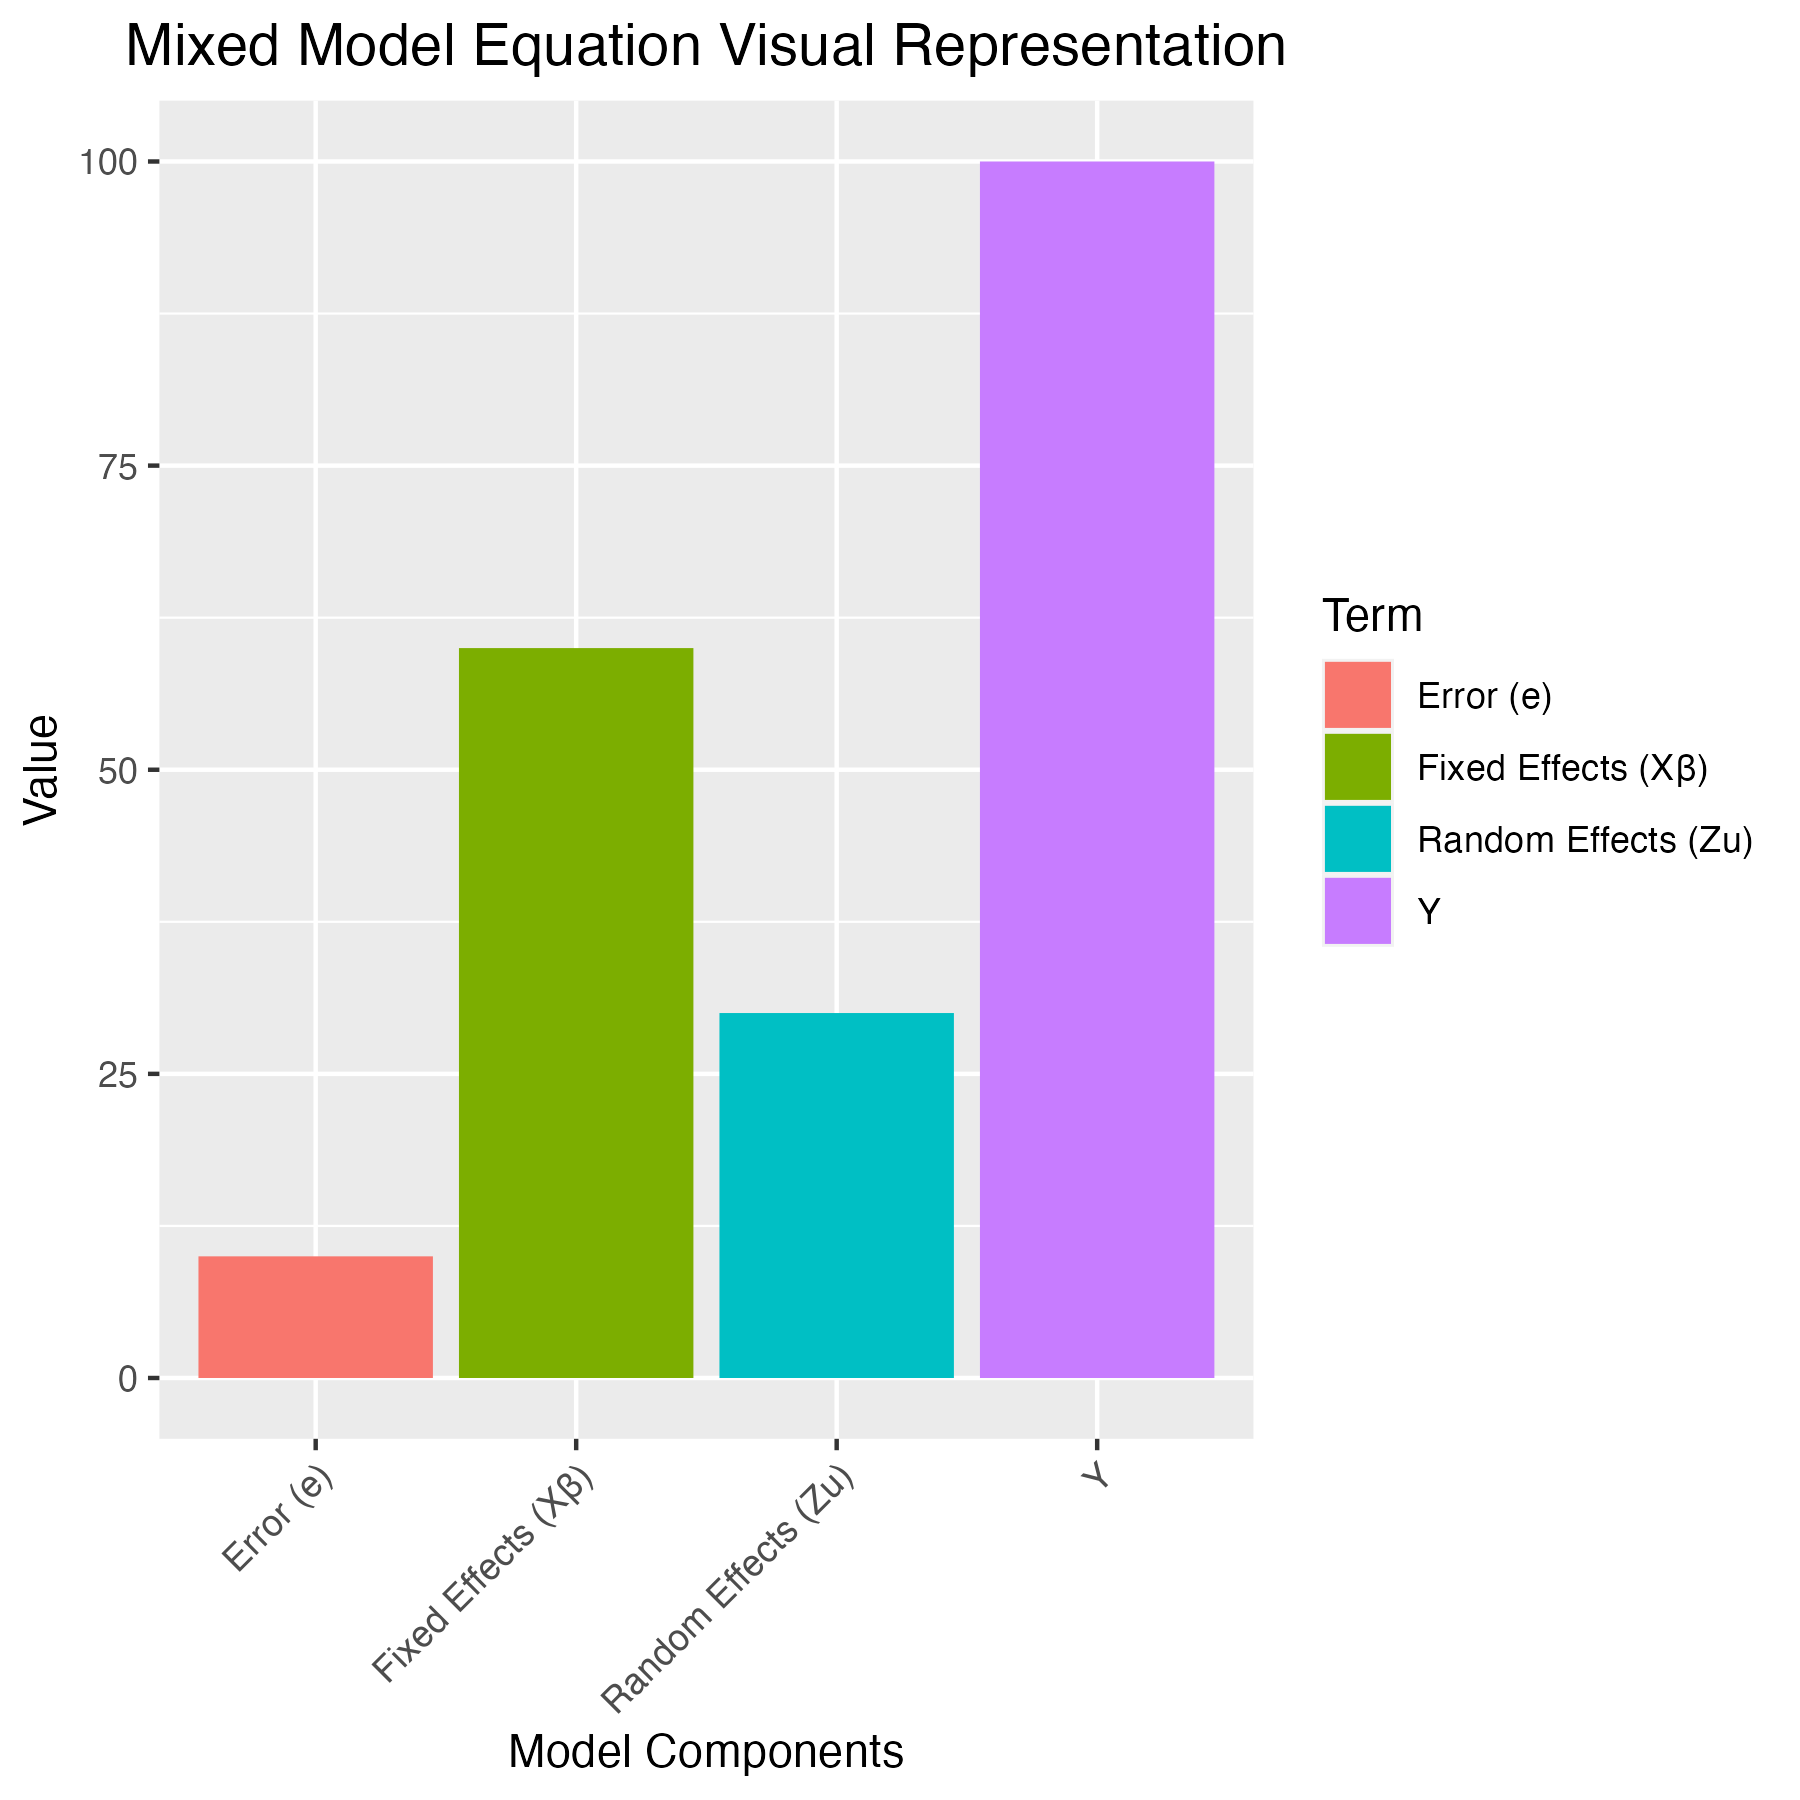
\includegraphics[width=0.8\textwidth]{mixed_model_visual.png}
    \caption{Mixed model equation visual representation: illustrates the contributions of error, fixed effects, random effects, and response variable \( Y \) in the model.}
    \label{fig:mixed-model-visual}
\end{figure}

\subsubsection{Step 4: Calculating Prediction Error Variance}

For random effects, we also calculate the Prediction Error Variance (PEV):

\[
PEV(\hat{\mathbf{u}}) = \sigma^2_g\mathbf{K} - \sigma^4_g\mathbf{K}\mathbf{Z'P}\mathbf{Z}\mathbf{K}
\]

\begin{biologicalinsightbox}[Practical Application]
In plant breeding, PEV is crucial for calculating the reliability of genetic value predictions. Higher reliability (lower PEV) indicates more confidence in using a prediction for selection decisions.

In evolutionary genetics, PEV can inform us about the precision of our estimates of genetic parameters, helping to guide interpretations about evolutionary processes.
\end{biologicalinsightbox}

\begin{figure}[htbp]
  \centering
  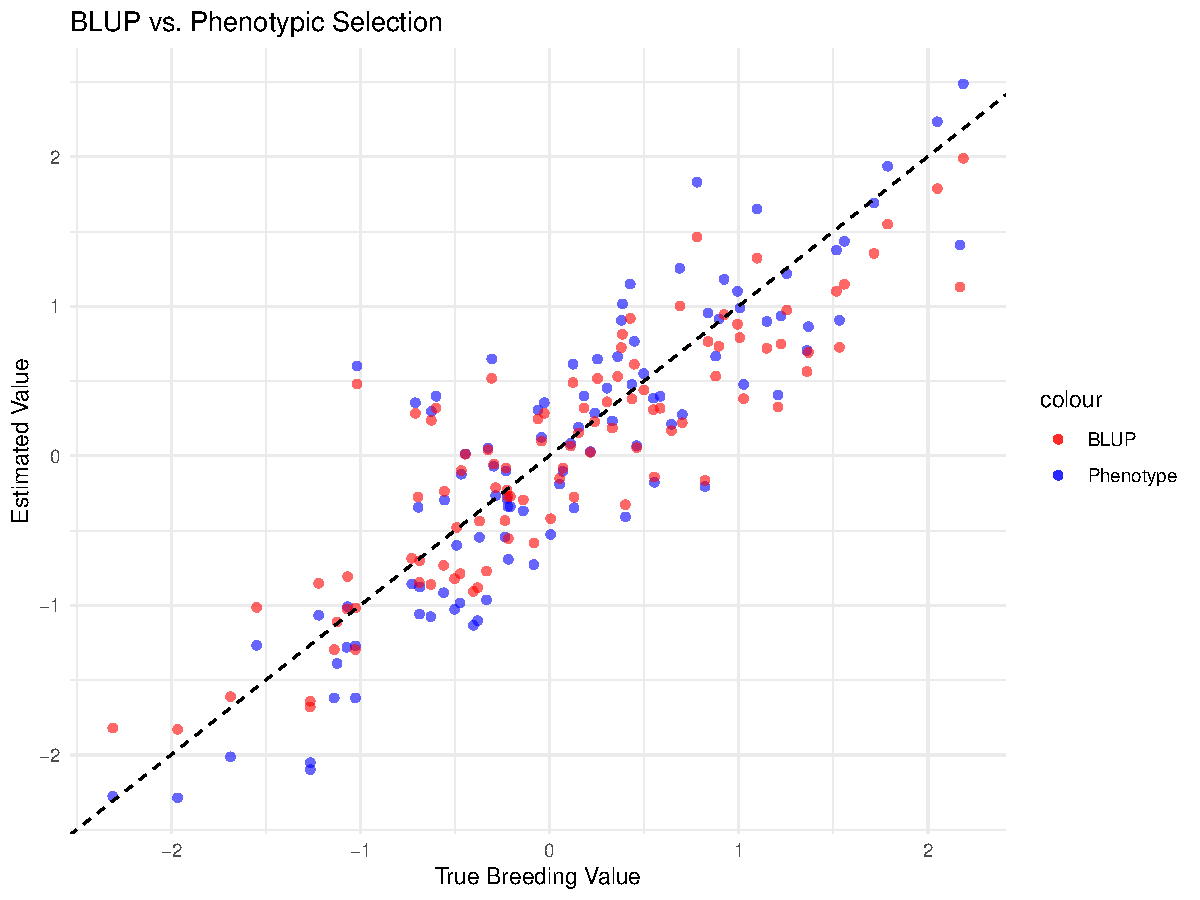
\includegraphics[width=0.8\textwidth]{blup_vs_phenotype.pdf}
  \caption{Comparison of BLUP estimates and phenotypic values against true breeding values}
  \label{fig:blup_vs_phenotype}
\end{figure}

\subsubsection{Step 5: Interpretation and Use of Results}

After obtaining the BLUEs, BLUPs, their standard errors, and PEV, we can use these results for various purposes:

\begin{enumerate}
    \item Ranking genotypes based on their predicted genetic values ($\hat{\mathbf{u}}$) for selection in breeding programs
    \item Estimating the effects of different environments or treatments ($\hat{\mathbf{b}}$) to optimize growing conditions or experimental designs
    \item  Calculating genetic parameters like heritability using the variance components estimated during the MME solution process
    \item Assessing the precision of our estimates and predictions using the standard errors and PEV to guide decision-making and further experimental planning
\end{enumerate}

\begin{keyconceptbox}
Solving Henderson's MME allows us to disentangle genetic and environmental effects, providing valuable insights for both applied breeding programs and fundamental evolutionary studies. The ability to simultaneously estimate fixed effects and predict random effects, while accounting for the genetic relationships between individuals, makes this approach powerful and widely applicable in biological research.
\end{keyconceptbox}

\section{Worked Example: Mixed Model Equations in Evolutionary Genetics}

Mixed models are widely used in evolutionary genetics to account for both fixed effects (e.g., environmental variables) and random effects (e.g., genetic variation within populations).

\subsection{Basic Mixed Model Framework}

The general form of a mixed model is:
\[
y = X\beta + Z\gamma + \epsilon
\]
Where:
\begin{itemize}
    \item \( y \) is the vector of phenotypic observations (e.g., trait measurements),
    \item \( X \) is the design matrix for fixed effects (e.g., environmental variables),
    \item \( Z \) is the design matrix for random effects (e.g., genetic or spatial structure),
    \item \( \beta \) is the vector of fixed effects,
    \item \( \gamma \) is the vector of random effects (e.g., genetic relatedness), and
    \item \( \epsilon \) represents residual error.
\end{itemize}

\subsection{Example 1: Modelling Trait Variation Across Populations}

In this example, we model phenotypic variation (e.g., flowering time) across different populations of a species. Fixed effects include environmental factors such as temperature and rainfall, while random effects account for population structure (e.g., different gene pools across populations).

\begin{example}[Trait Variation in Populations]
Consider a study on the flowering time of a plant species across multiple populations that inhabit different environments. The mixed model equation would be:
\[
\text{Flowering Time} = \beta_0 + \beta_1 \text{Temperature} + \beta_2 \text{Rainfall} + u_j + \epsilon
\]
Where \( u_j \) represents the random effect of population \( j \). This accounts for the fact that genetic differences between populations can contribute to variation in flowering time.
\end{example}

See the \textbf{Appendix: Simulating and Analysing Mixed Models in R} for an illustration of how to run this model in R with a simulated population. The next two figures show results from this example that you can obtain by running the code in the appendix. 

\begin{figure}[h]
\centering
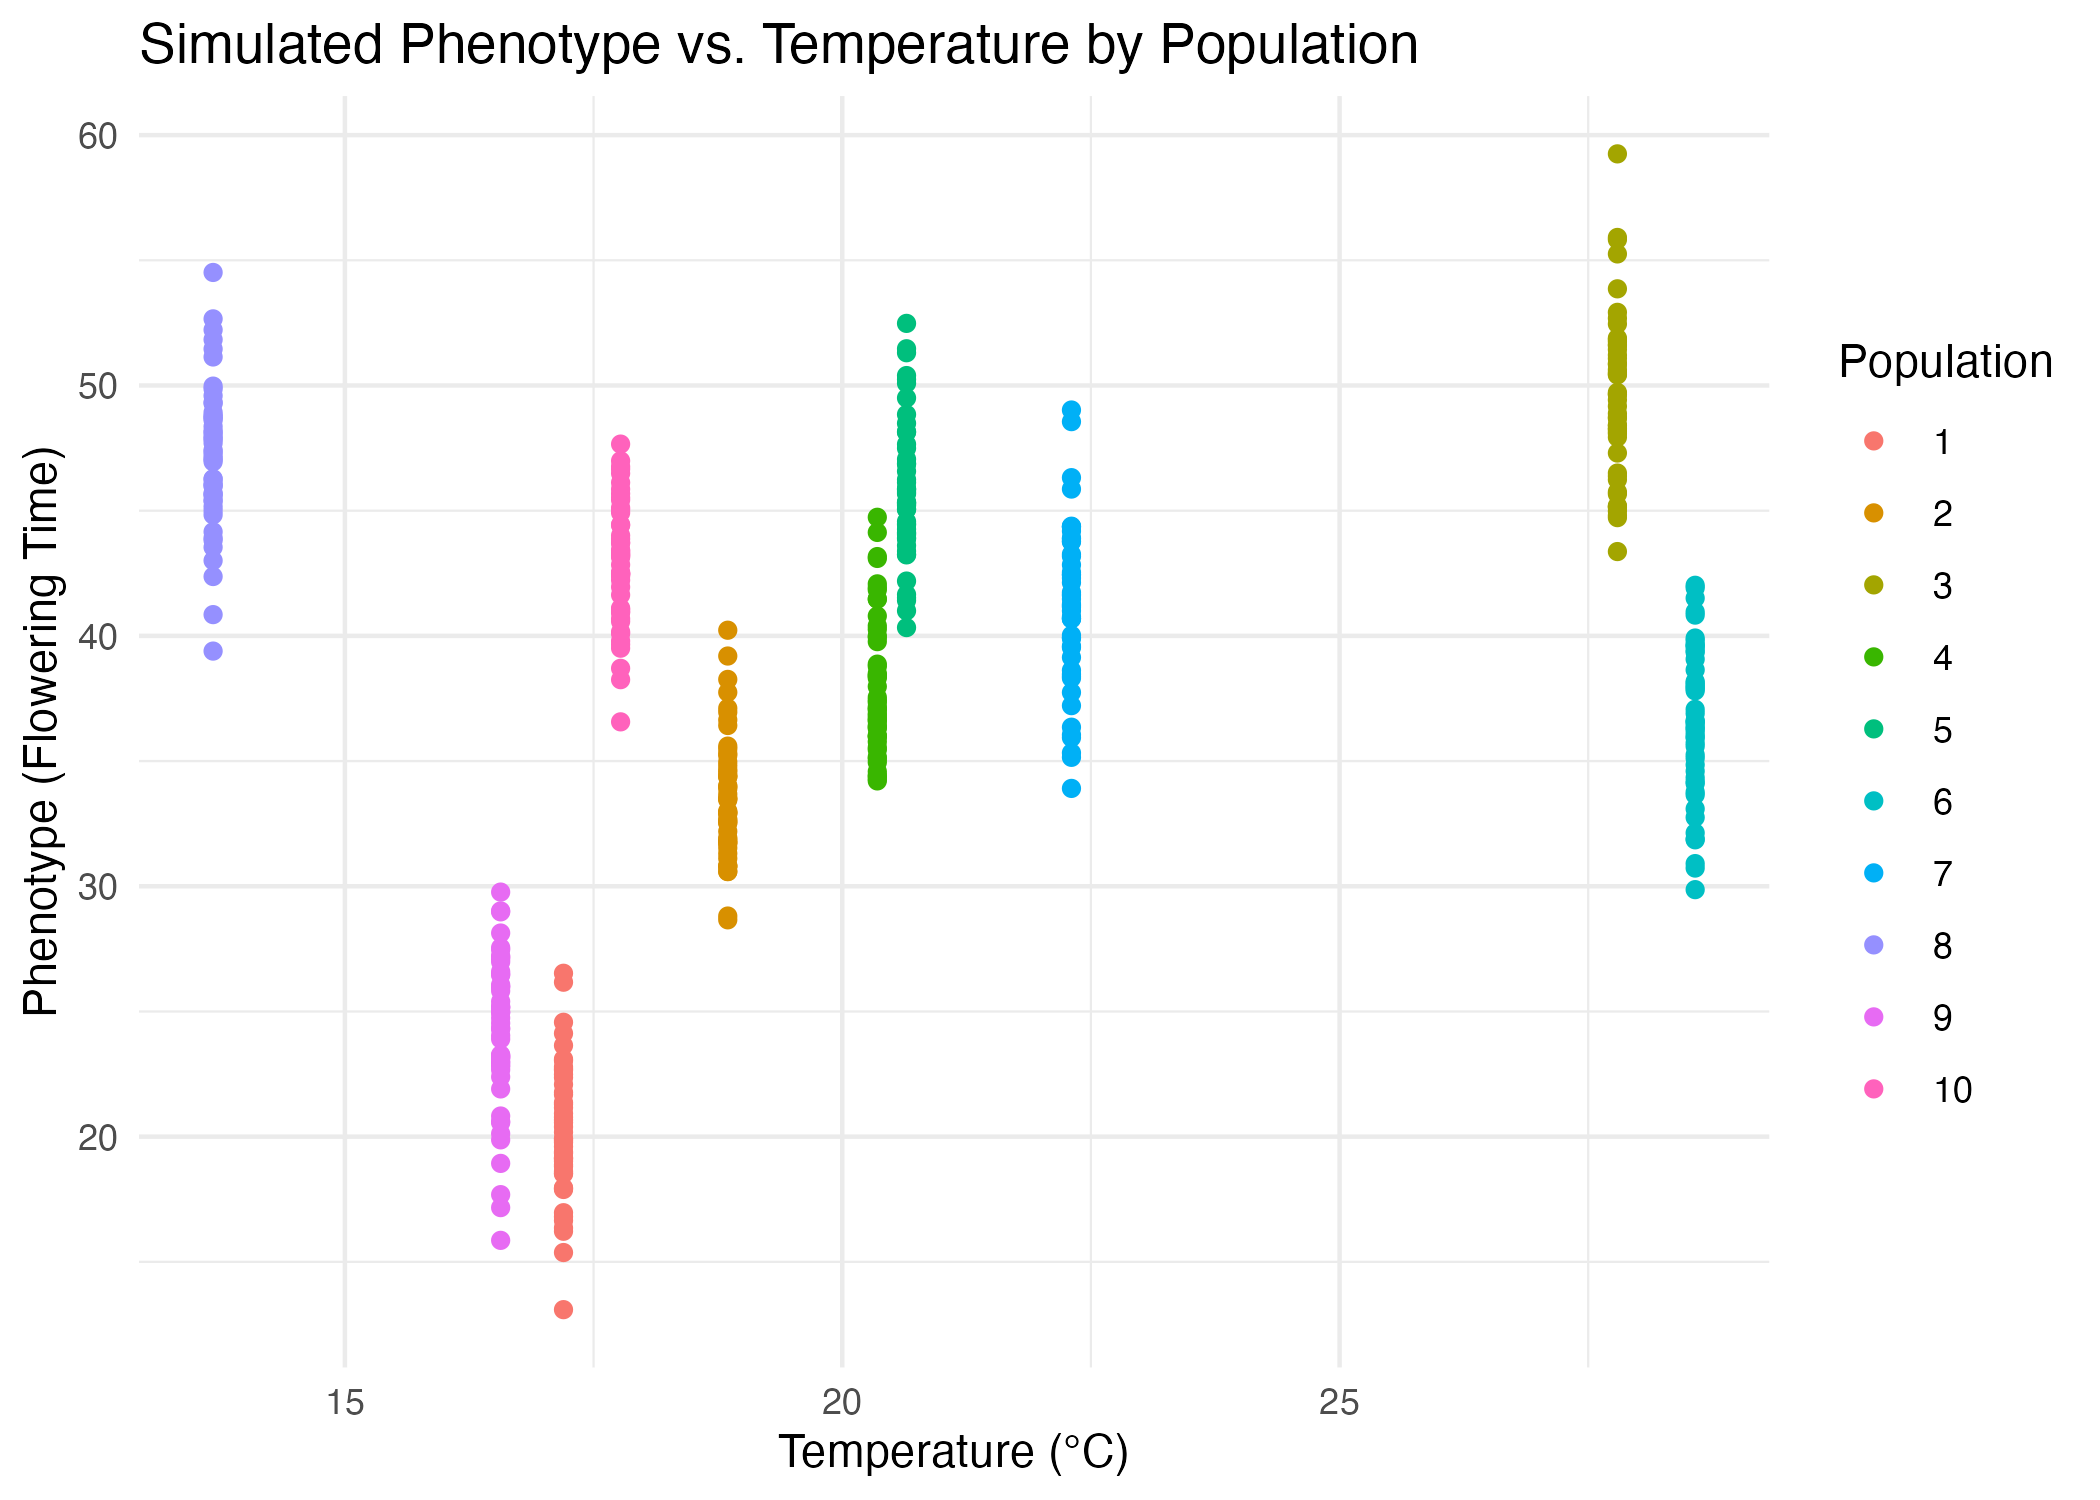
\includegraphics[width=0.8\textwidth]{simulated_phenotype_vs_temperature.png}
\caption{Simulated Phenotype vs. Temperature by Population}
\end{figure}

\begin{figure}[h]
\centering
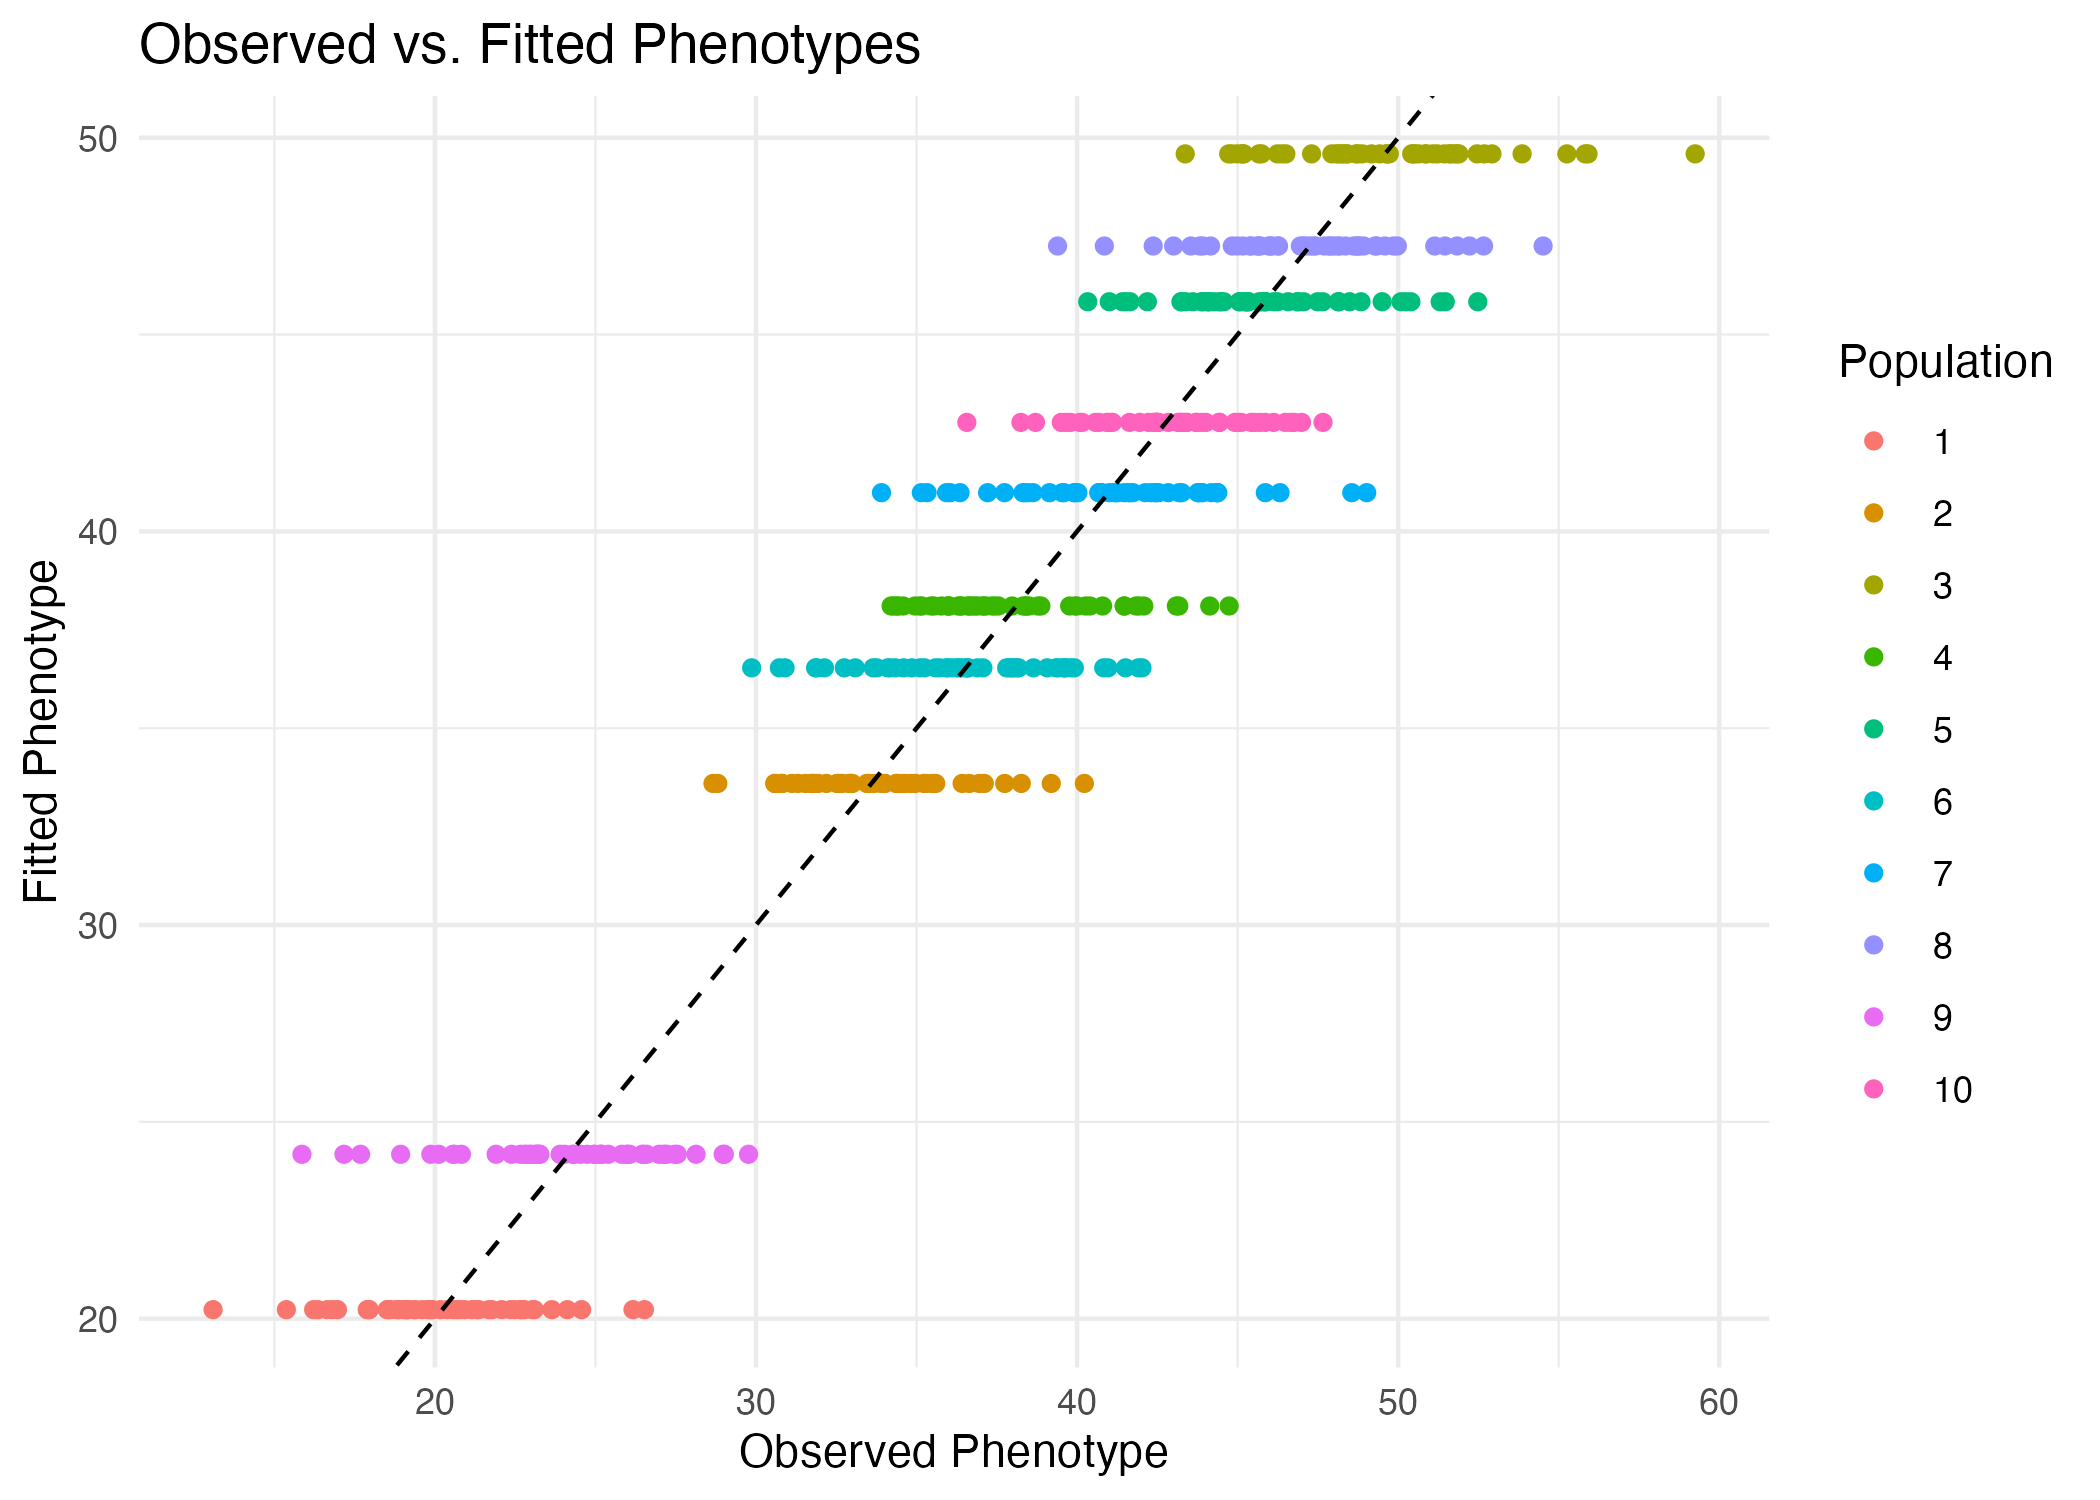
\includegraphics[width=0.8\textwidth]{observed_vs_fitted_phenotypes.png}
\caption{Observed vs. Fitted Phenotypes}
\end{figure}

\begin{interpretation}[Biological Interpretation: Heritability in Evolutionary Genetics]
Heritability estimates the proportion of trait variation that is due to genetic factors, as opposed to environmental factors. In evolutionary genetics, high heritability for a trait like flowering time suggests that the trait can respond rapidly to natural selection. Conversely, if heritability is low, environmental factors may play a more dominant role, limiting the potential for rapid evolutionary change.
\end{interpretation}

\subsection{Example 2: Gene Flow and Local Adaptation}

In this example, we investigate gene flow and local adaptation by modelling the fitness of individuals as a function of environmental gradients and genetic variation. Here, genetic effects are random, while environmental gradients (e.g., soil moisture) are fixed.

\begin{example}[Gene Flow and Local Adaptation]
We model fitness in terms of reproductive success across an environmental gradient (e.g., soil moisture). Genetic variation within populations is treated as a random effect, while soil moisture is a fixed effect.
\[
\text{Fitness} = \beta_0 + \beta_1 \text{Soil Moisture} + u_i + \epsilon
\]
Here, \( u_i \) is the random effect for individual \( i \), capturing genetic variation, and \( \epsilon \) is the residual error. This model helps assess how much of the variation in fitness is due to local adaptation versus random genetic drift.
\end{example}

\subsection{Example 3: Spatially Structured Populations}

In many evolutionary genetics studies, individuals may be spatially structured, which affects gene flow and selection pressures. This model accounts for spatial autocorrelation by including spatial location as a random effect.

\begin{example}[Spatial Structure in Evolutionary Genetics]
We model the phenotypic trait height across a spatially structured population. Spatial location is treated as a random effect to account for spatial autocorrelation in trait values.
\[
\text{Height} = \beta_0 + \beta_1 \text{Elevation} + u_{\text{location}} + \epsilon
\]
Where \( u_{\text{location}} \) represents the random effect of spatial location, accounting for the fact that nearby individuals may share similar trait values due to both genetic and environmental factors.
\end{example}

\subsection{Example 4: Selection and Genetic Relatedness}

Mixed models are frequently used to quantify selection on traits by including relatedness between individuals as a random effect. This helps control for shared ancestry when estimating selection gradients.

\begin{example}[Selection on Traits with Genetic Relatedness]
We investigate selection on plant height within a population by modelling height as a function of environmental factors and relatedness. The mixed model is:
\[
\text{Height} = \beta_0 + \beta_1 \text{Light Availability} + u_k + \epsilon
\]
Where \( u_k \) is the random effect for genetic relatedness among individuals. This allows us to estimate the effect of environmental variables on height while accounting for shared ancestry.
\end{example}

\begin{interpretation}[Biological Interpretation: Multivariate Traits in Plant Breeding]
Many plant traits, such as yield and drought resistance, are influenced by multiple factors simultaneously. The multivariate normal distribution allows breeders to model these traits together, understanding how they co-vary across individuals. This is crucial when selecting for multiple traits at once, as it helps breeders understand trade-offs—such as whether selecting for high yield may inadvertently reduce drought resistance.
\end{interpretation}


\subsection{Conclusion}

Mixed models provide a flexible framework to account for the complex interactions between environmental factors and genetic structure in evolutionary genetics. By incorporating both fixed and random effects, researchers can better understand the relative contributions of different factors to phenotypic variation and fitness.

\section{Summary of BLUEs and BLUPs}

\begin{table}[htbp]
\centering
\footnotesize
\begin{tabularx}{\textwidth}{|>{\hsize=0.8\hsize}X|>{\hsize=1.1\hsize}X|>{\hsize=1.1\hsize}X|}
\hline
\textbf{Aspect} & \textbf{BLUEs (Fixed Effects)} & \textbf{BLUPs (Random Effects)} \\
\hline
Solution & $\mathbf{b} = (\mathbf{X'V}^{-1}\mathbf{X})^- \mathbf{X'V}^{-1}\mathbf{y}$ & $\mathbf{u} = \sigma^2_g\mathbf{KZ'V}^{-1}(\mathbf{y} - \mathbf{Xb})$ \\
\hline
Properties & \multicolumn{2}{>{\hsize=2.2\hsize}X|}{Best: Minimum variance among unbiased estimators/predictors. 
Linear: Formed from a linear combination of observations.} \\
\cline{2-3}
 & $E(\mathbf{b}) = \mathbf{b}$ & $E(\mathbf{u}) = 0$ \\
\hline
Plant Breeding Interpretation & Unbiased estimates of environmental effects & Predictions of genetic values for plant lines or varieties \\
\hline
Evolutionary Genetics Interpretation & Estimates of selection gradients or fitness effects & Estimates of breeding values or population-specific deviations \\
\hline
Key Advantage & Accounts for genetic covariance among populations & Incorporates genetic relationships, improving prediction accuracy \\
\hline
\end{tabularx}
\caption{Summary of Best Linear Unbiased Estimates (BLUEs) and Best Linear Unbiased Predictions (BLUPs)}
\label{tab:blues_blups_summary}
\end{table}

\begin{keyconceptbox}
    
BLUEs and BLUPs provide a powerful framework for separating and estimating environmental and genetic effects in complex biological systems. Their properties ensure optimal use of available data, making them invaluable tools in both applied plant breeding and fundamental evolutionary research.
\end{keyconceptbox}

\textbf{Note on Variance-Covariance Matrix:} In both solutions, $\mathbf{V} = \sigma^2_g\mathbf{ZKZ'} + \sigma^2_e\mathbf{I}$ is the variance-covariance matrix of the observations, where $\sigma^2_g$ is the genetic variance, $\mathbf{K}$ is the kinship matrix, $\sigma^2_e$ is the residual variance, and $\mathbf{I}$ is the identity matrix.

\begin{figure}[h]
    \centering
    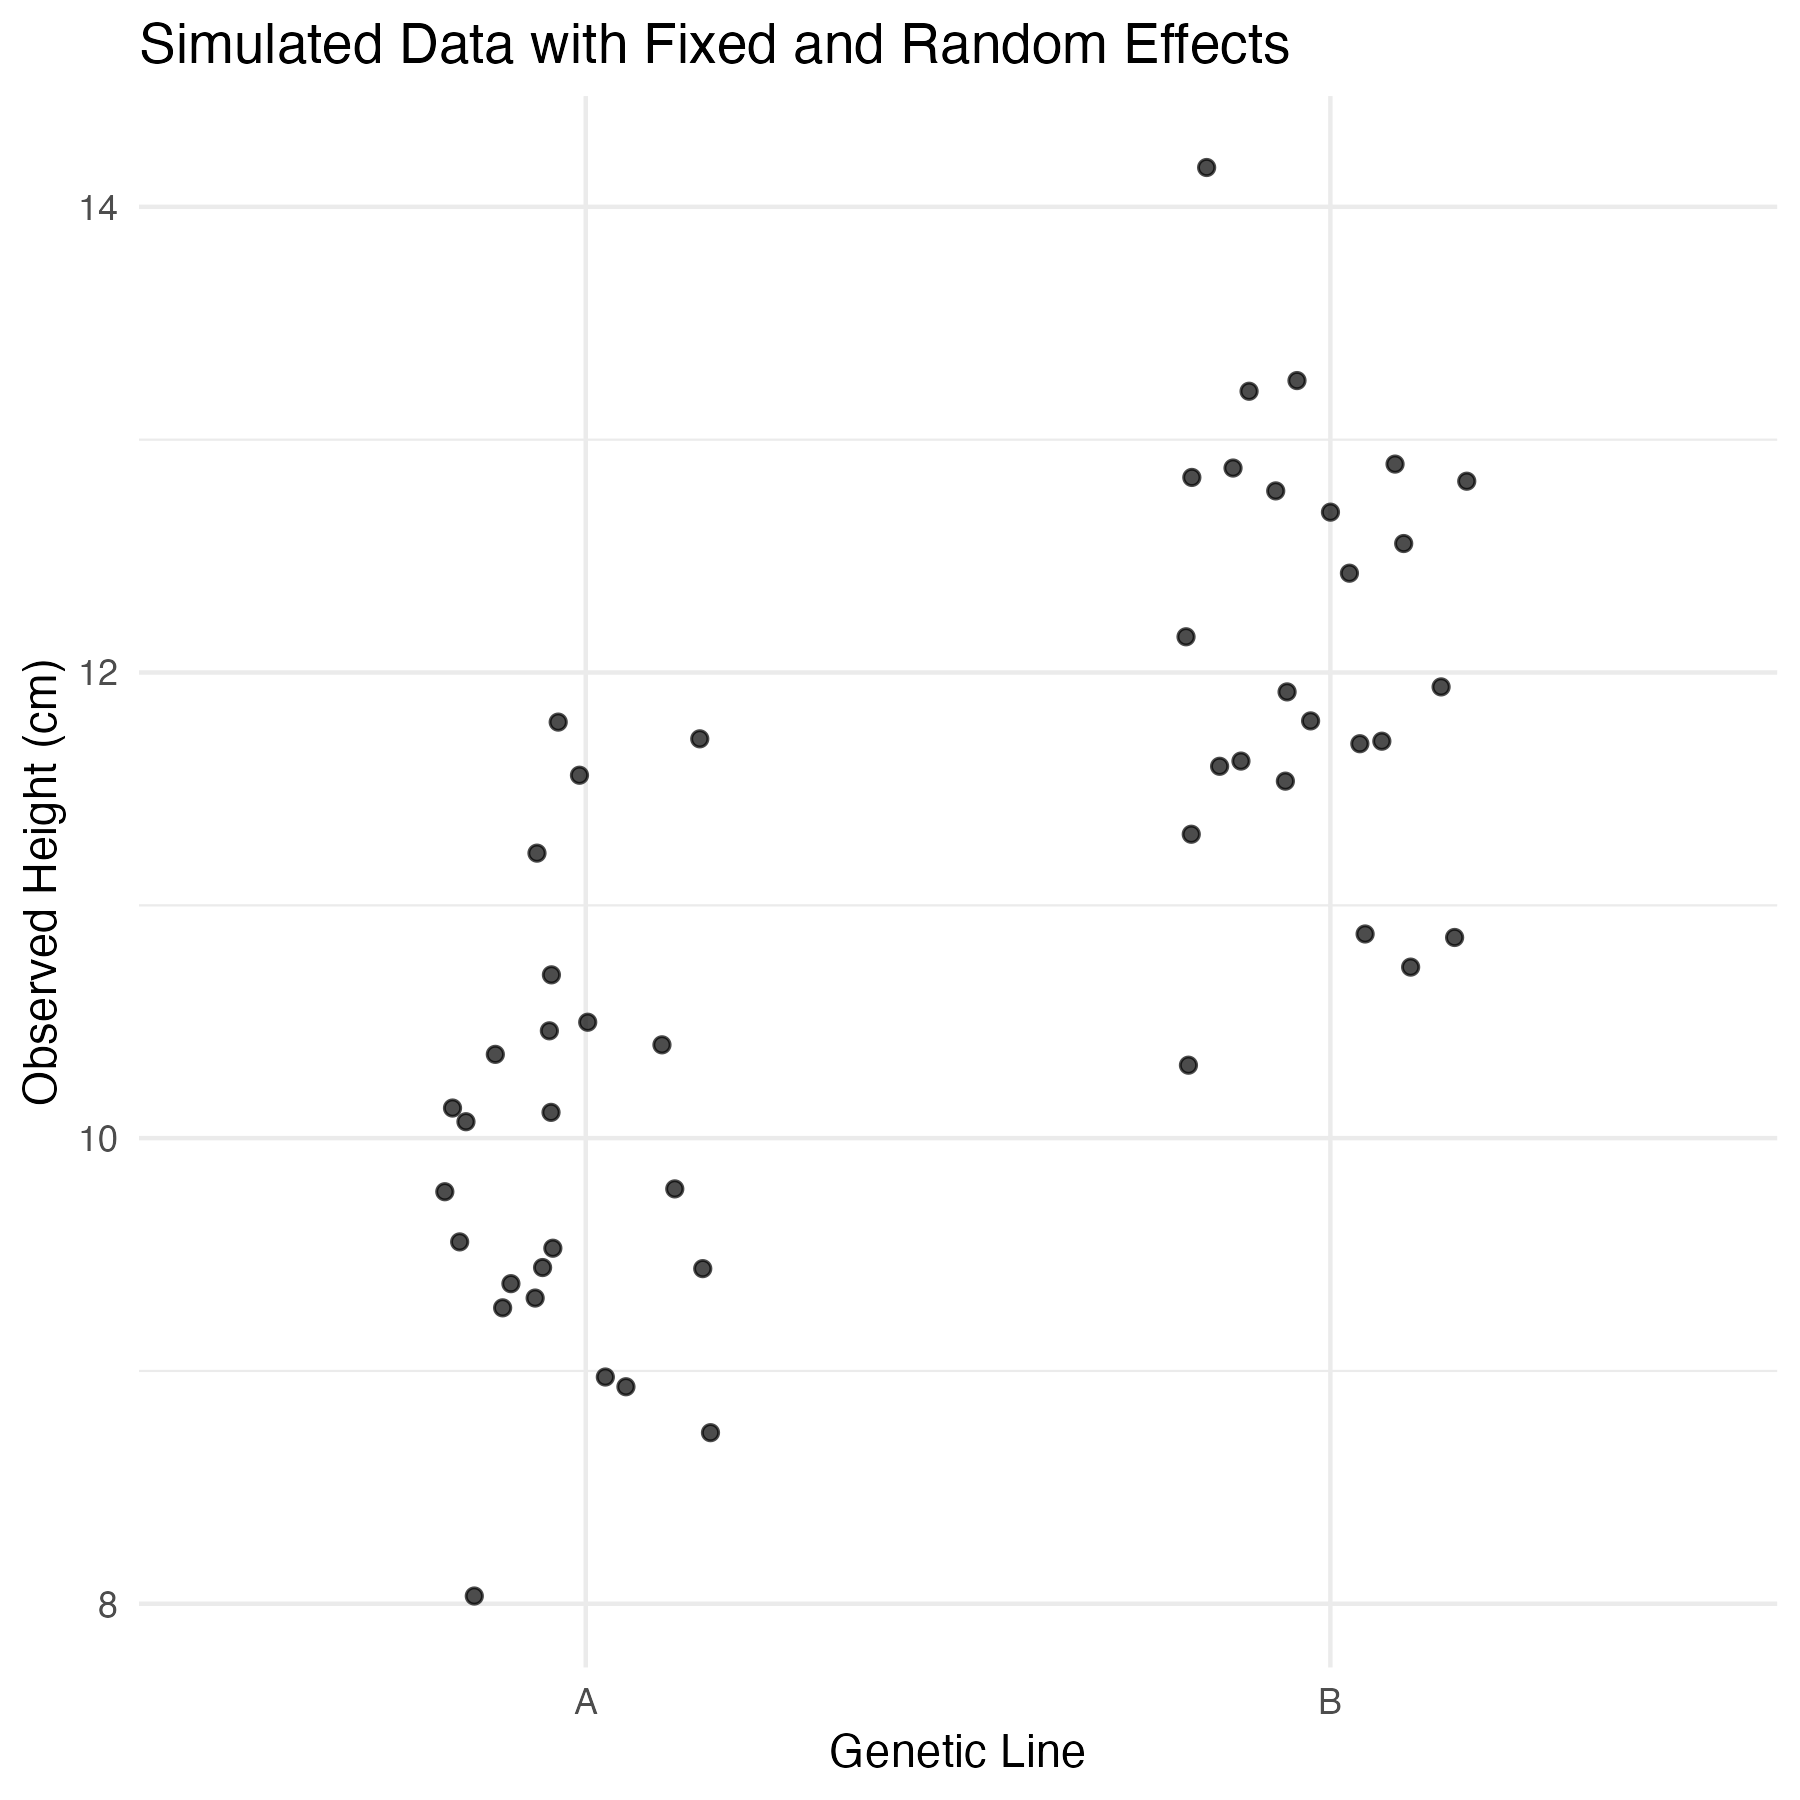
\includegraphics[width=0.8\textwidth]{random_effects_simulation.png}
    \caption{Random effects simulation results: distribution of values for groups A and B highlighting the variability in random effects estimates.}
    \label{fig:random-effects-simulation}
\end{figure}

\section{Connecting Lande's Equation with Mixed Model Equations}

Both Lande’s Equation and Mixed Model Equations (MME) are foundational to understanding the genetic architecture of traits and their evolution under selection pressures. Lande’s Equation is a key tool in evolutionary biology, predicting the response to selection in quantitative traits, while MME is used in quantitative genetics to estimate breeding values (random effects) and environmental effects (fixed effects) by accounting for genetic relationships in phenotypic data.

\subsection{Lande's Equation in Quantitative Genetics}

Lande's equation extends the univariate breeder's equation into a multivariate framework, allowing for the genetic variance-covariance structure across multiple traits:
\[
\Delta \mathbf{z} = \mathbf{G} \boldsymbol{\beta}
\]
Where:
\begin{itemize}
    \item \( \Delta \mathbf{z} \) represents the vector of changes in trait means over time.
    \item \( \mathbf{G} \) is the genetic variance-covariance matrix for the traits of interest.
    \item \( \boldsymbol{\beta} \) is the selection gradient, which describes the intensity and direction of selection on the traits.
\end{itemize}
This equation models how traits respond to selection in a population, incorporating multiple traits and their genetic correlations.

\subsection{Mixed Model Equations and Genetic Architecture}

Mixed Model Equations (MME) provide a statistical framework to decompose phenotypic variation into genetic and environmental components. The general form of MME is expressed as:
\[
\mathbf{y} = \mathbf{X} \boldsymbol{\beta} + \mathbf{Z} \mathbf{u} + \boldsymbol{\epsilon}
\]
Where:
\begin{itemize}
    \item \( \mathbf{y} \) is the vector of observed phenotypes.
    \item \( \boldsymbol{\beta} \) represents the fixed effects, such as environmental factors or overall means.
    \item \( \mathbf{u} \) represents the random effects, typically the breeding values of individuals.
    \item \( \boldsymbol{\epsilon} \) is the residual error, accounting for unobserved environmental variation.
\end{itemize}
The random effects \( \mathbf{u} \) are assumed to follow a multivariate normal distribution with a mean of 0 and variance \( \mathbf{G} \), which is the genetic variance-covariance matrix used in Lande’s equation. 

\subsection{Bridging the Gap: Connecting Lande’s Equation and MME}

The link between Lande’s equation and MME lies in the shared genetic variance-covariance matrix \( \mathbf{G} \). In both Lande’s equation and MME:
\begin{itemize}
    \item The matrix \( \mathbf{G} \) determines how genetic variation influences the response to selection.
    \item Lande’s equation uses \( \mathbf{G} \) to describe the evolutionary response to selection pressures.
    \item MME uses \( \mathbf{G} \) to estimate random effects, allowing prediction of genetic merit or breeding values in populations.
\end{itemize}
Thus, both frameworks model the same underlying genetic architecture, though Lande’s equation focuses on evolutionary change, while MME is primarily concerned with estimating breeding values and environmental contributions.

\begin{keyconceptbox}[Lande's Equation and MME]
Lande’s equation and MME share a common genetic foundation through the genetic variance-covariance matrix \( \mathbf{G} \). Both approaches model how traits respond to selection, either through evolutionary dynamics (Lande’s equation) or phenotypic predictions (MME).
\end{keyconceptbox}

\subsection{Using Lande’s Equation within the MME Framework}

The combination of MME and Lande’s equation provides a comprehensive approach for predicting evolutionary and breeding outcomes. Here, we outline the steps to connect these two frameworks:

\subsubsection{Step 1: Estimating Genetic Values Using MME}

In the MME framework, the random effects \( \mathbf{u} \) (representing genetic values or breeding values) are estimated by solving the mixed model equations:
\[
\mathbf{u} = \mathbf{G} \mathbf{Z}^\top \mathbf{V}^{-1} (\mathbf{y} - \mathbf{X} \boldsymbol{\beta})
\]
Where:
\begin{itemize}
    \item \( \mathbf{G} \) is the genetic variance-covariance matrix.
    \item \( \mathbf{V} \) is the total variance-covariance matrix, incorporating genetic and residual variance.
    \item \( \mathbf{Z} \) is the design matrix for random effects.
    \item \( \mathbf{X} \) is the design matrix for fixed effects.
    \item \( \mathbf{y} \) is the vector of observed phenotypes.
\end{itemize}
The resulting \( \hat{\mathbf{u}} \) represents the predicted breeding values or genetic effects for each individual.

\subsubsection{Step 2: Applying Lande’s Equation to Predict Evolutionary Change}

Once genetic values are estimated using MME, we can apply Lande’s equation to predict the response to selection. Using the estimated genetic variance-covariance matrix \( \hat{\mathbf{G}} \) and selection gradient \( \boldsymbol{\beta} \), Lande’s equation is expressed as:
\[
\Delta \mathbf{z} = \hat{\mathbf{G}} \boldsymbol{\beta}
\]
Where:
\begin{itemize}
    \item \( \Delta \mathbf{z} \) is the vector of expected changes in the mean traits.
    \item \( \hat{\mathbf{G}} \) is the estimated genetic variance-covariance matrix.
    \item \( \boldsymbol{\beta} \) is the selection gradient, often calculated from estimated breeding values.
\end{itemize}
This approach predicts how selection on multiple traits will change the population’s trait means, accounting for both direct selection on individual traits and genetic correlations between traits.

\subsubsection{Step 3: Predicting the Response to Selection}

Finally, combining the MME framework with Lande’s equation allows us to predict the joint response of traits to selection. For trait \( i \), the response to selection is predicted as:
\[
\Delta z_i = G_{ii} \beta_i
\]
And for multiple traits:
\[
\Delta \mathbf{z} = \mathbf{G} \boldsymbol{\beta}
\]
Thus, both genetic variances (\( G_{ii} \)) and covariances (\( G_{ij} \)) play a role in predicting how traits evolve under selection.

\begin{keyconceptbox}[Application of Lande’s Equation in MME]
Lande’s equation can be integrated into the MME framework by using MME-derived estimates of genetic values and variance-covariance matrices. This combined approach provides powerful tools for predicting both short-term breeding outcomes and long-term evolutionary changes.
\end{keyconceptbox}

\subsection{Worked Example: Simulating Phenotypic Data and Estimating Genetic Parameters}

In the following example, we simulate phenotypic data for two traits across multiple populations and families. We then estimate the genetic variance-covariance matrix \( \mathbf{G} \) using mixed models and apply Lande’s equation to predict the response to selection. The R code used for this simulation and analysis is included in the appendix.

By combining these theoretical frameworks, we gain a deeper understanding of both the short-term genetic changes that affect breeding outcomes and the long-term evolutionary dynamics of quantitative traits.


\section{Genomic Best Linear Unbiased Prediction (GBLUP)}

As molecular technologies have advanced, the integration of genomic information into breeding programs and evolutionary studies has become increasingly important. Genomic Best Linear Unbiased Prediction (GBLUP) represents a significant extension of the traditional BLUP methodology, incorporating dense genetic marker data to enhance prediction accuracy. This section explores the principles of GBLUP and its applications in plant breeding and evolutionary genetics.

\subsection{From BLUP to GBLUP}

Traditional BLUP relies on pedigree information to construct the kinship matrix, which represents the expected genetic relationships between individuals. GBLUP, on the other hand, uses genomic data to estimate realized genetic relationships more accurately.

\begin{keyconceptbox}
    GBLUP replaces the pedigree-based relationship matrix (A) used in traditional BLUP with a genomic relationship matrix (G) derived from molecular marker data.

\end{keyconceptbox}

This transition from expected to realized relationships can significantly improve prediction accuracy, especially for complex traits controlled by many genes.

\subsection{The Genomic Relationship Matrix}

The genomic relationship matrix (G) is at the heart of GBLUP. It is constructed using genome-wide marker data, typically single nucleotide polymorphisms (SNPs). The basic form of the G matrix can be calculated as:

\[
\mathbf{G} = \frac{\mathbf{ZZ'}}{2\sum_{j=1}^m p_j(1-p_j)}
\]

Where:
\begin{itemize}
    \item $\mathbf{Z}$ is a matrix of centered genotype scores
    \item $p_j$ is the minor allele frequency for the $j$-th SNP
    \item $m$ is the total number of SNPs
\end{itemize}

\subsection{GBLUP Model}

\begin{keyconceptbox}
The basic GBLUP model can be represented as:

\[
\mathbf{y} = \mathbf{X\beta} + \mathbf{Zg} + \mathbf{e}
\]

Where:
\begin{itemize}
    \item $\mathbf{y}$ is the vector of phenotypes
    \item $\mathbf{X}$ is the design matrix for fixed effects
    \item $\mathbf{\beta}$ is the vector of fixed effects
    \item $\mathbf{Z}$ is the design matrix for random effects
    \item $\mathbf{g}$ is the vector of genomic breeding values
    \item $\mathbf{e}$ is the vector of residuals
\end{itemize}

The key assumption in GBLUP is:

\[
\mathbf{g} \sim N(0, \mathbf{G}\sigma_g^2)
\]

Where $\sigma_g^2$ is the genetic variance and $\mathbf{G}$ is the genomic relationship matrix.
\end{keyconceptbox}
The following flowchart summarises the required steps to calculate genomic breeding values using MME and GRM.\\

\begin{figure}[h]
    \centering
    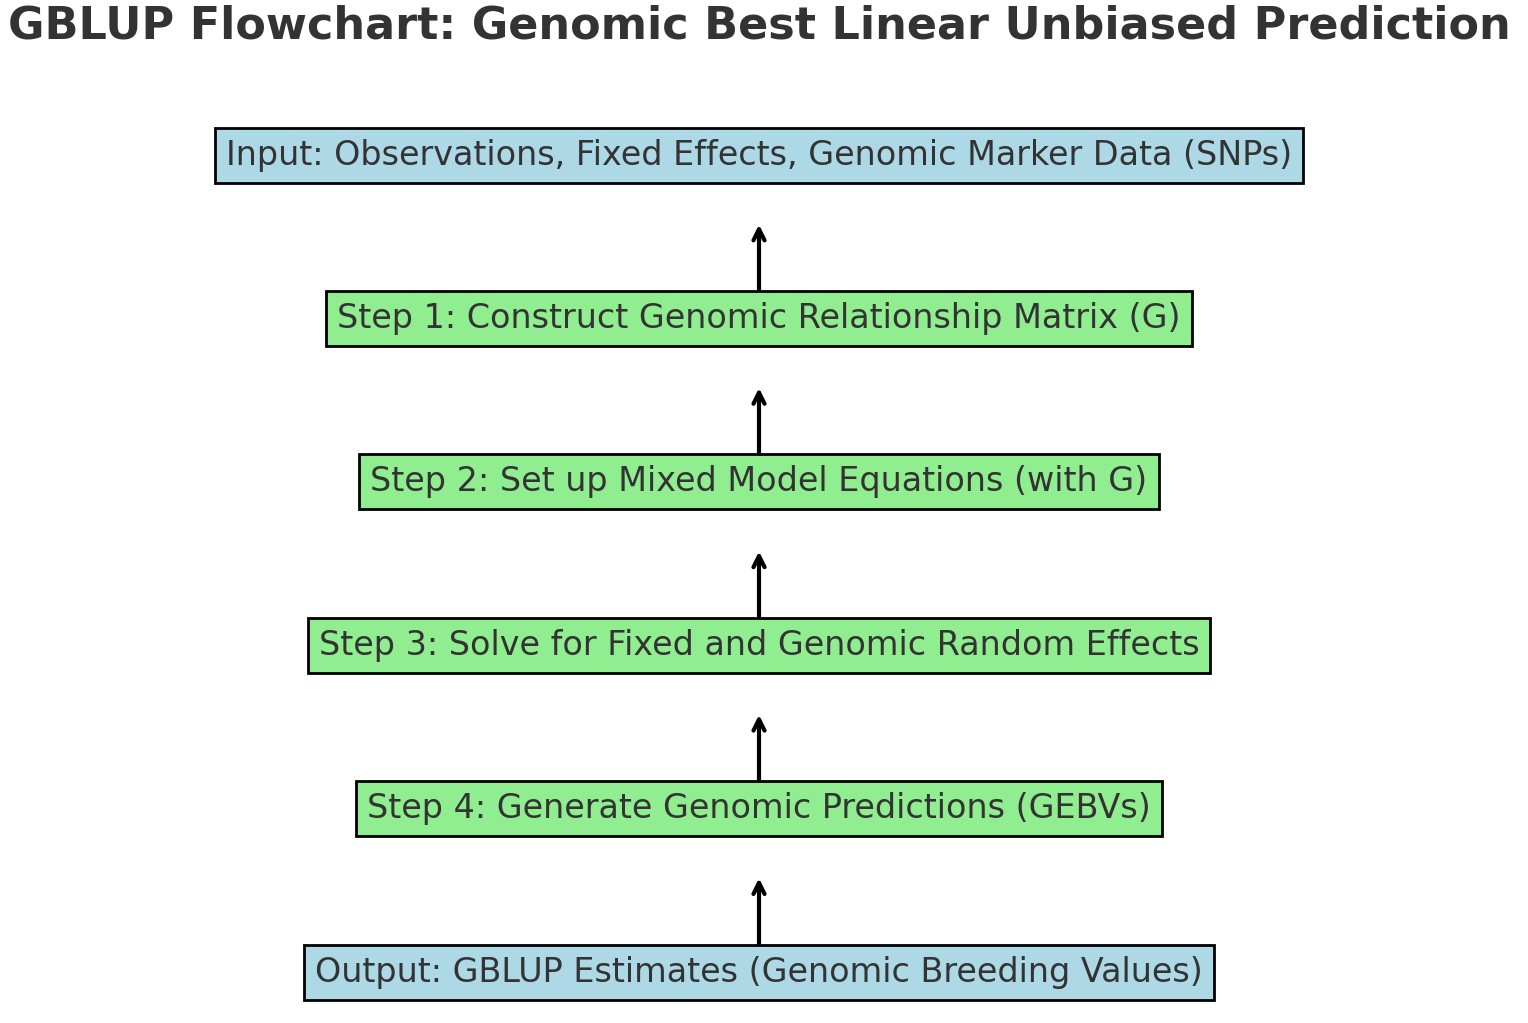
\includegraphics[width=1\textwidth]{gblupFC.jpg}
    \caption{GBLUP flowchart showing the process of generating genomic breeding values (GEBVs) using genomic relationship matrices and mixed model equations.}
    \label{fig:gblup-flowchart}
\end{figure}

\subsection{Advantages of GBLUP}

Genomic Best Linear Unbiased Prediction (GBLUP) represents a significant advancement over traditional BLUP methods, offering several key advantages that have revolutionized both plant breeding programs and evolutionary genetics studies. At the heart of GBLUP's power is its ability to capture realized genetic relationships with unprecedented accuracy. This improvement stems from the use of dense genetic markers, typically single nucleotide polymorphisms (SNPs), which provide a high-resolution picture of genetic similarity between individuals. One of the most striking benefits of GBLUP is its improved prediction accuracy, particularly for individuals with limited or no phenotypic data. In plant breeding, this means that breeders can make informed decisions about which lines to advance in their program even before extensive field trials are conducted. For example, a breeder working on drought-resistant wheat could use GBLUP to predict the performance of newly developed lines based on their genetic similarity to known high-performing varieties, potentially saving years in the breeding cycle.

GBLUP also excels in accounting for Mendelian sampling, a feature that sets it apart from pedigree-based BLUP. This capability allows GBLUP to differentiate between full siblings, which share the same pedigree but may have inherited different combinations of parental alleles. In evolutionary genetics, this fine-grained differentiation enables researchers to better understand and model the genetic basis of trait variation within families, providing insights into processes like adaptive radiation in closely related species. Another significant advantage of GBLUP is its ability to capture distant historical relationships that may not be evident in recent pedigrees. This feature is particularly valuable in evolutionary studies, where it can reveal cryptic relatedness between populations or species that appear distinct based on recent history alone. For instance, in studying the evolution of C4 photosynthesis in grasses, GBLUP could help identify shared genetic architectures between distantly related C4 species, shedding light on the parallel evolution of this complex trait.

The flexibility of GBLUP further enhances its utility across diverse applications. It can be readily extended to incorporate additional genomic information, such as known functional variants or epigenetic markers, providing a more comprehensive model of genetic architecture. In multi-trait scenarios, common in both breeding and evolutionary studies, GBLUP can simultaneously model multiple correlated traits, offering a more holistic view of genetic effects. This flexibility is crucial in tackling complex challenges like breeding for climate resilience in crops, where multiple traits (e.g., drought tolerance, heat resistance, and yield stability) must be considered simultaneously. By leveraging these advantages, GBLUP has become an indispensable tool in modern quantitative genetics. It bridges the gap between molecular data and phenotypic outcomes, offering unprecedented insights into genetic architecture and enabling more efficient and accurate selection in both natural and artificial evolutionary processes. As genomic technologies continue to advance, the power and applicability of GBLUP are likely to grow, further accelerating progress in plant breeding and deepening our understanding of evolutionary dynamics.

\begin{keyconceptbox}[Practical Impact]
GBLUP has enhanced plant breeding by enabling more efficient selection of superior genotypes, potentially accelerating genetic gain and reducing the time and cost of breeding cycles.
\end{keyconceptbox}

\subsection{Applications in Plant Breeding and Evolutionary Genetics}

The power of Genomic Best Linear Unbiased Prediction (GBLUP) has revolutionized both plant breeding and evolutionary genetics, offering unprecedented insights and capabilities in these fields. In plant breeding, GBLUP has become a cornerstone of genomic selection strategies, dramatically accelerating the breeding process and improving its efficiency. Breeders can now predict the performance of untested lines or hybrids with remarkable accuracy, allowing them to make informed decisions about which crosses to pursue without extensive field testing. For instance, in developing new high-yielding rice varieties, breeders can use GBLUP to predict the potential of thousands of possible crosses, focusing their efforts on the most promising combinations. This predictive power extends to optimizing crossing schemes, enabling breeders to strategically plan generations ahead, balancing the pursuit of desired traits with the maintenance of genetic diversity.

The application of GBLUP in plant breeding has significantly reduced the need for extensive field testing, especially in early generations. This not only saves time and resources but also allows for more rapid cycling through generations, accelerating the overall breeding process. For example, in developing disease-resistant wheat varieties, breeders can use GBLUP to predict resistance levels in early generations, quickly eliminating susceptible lines and focusing resources on the most promising candidates. This approach has proven particularly valuable in breeding for complex traits like drought tolerance or yield stability, where traditional phenotypic selection can be challenging and time-consuming. In the realm of evolutionary genetics, GBLUP and related methods have opened new avenues for understanding the genetic basis of adaptation and evolution. Researchers can now estimate the genomic heritability of complex traits with greater precision, shedding light on the proportion of trait variation attributable to genetic factors. This has been particularly insightful in studies of wild populations, where understanding the genetic architecture of adaptive traits is crucial. For instance, in studying the evolution of beak shape in Darwin's finches, GBLUP-based approaches have helped quantify the genomic basis of this iconic adaptive trait, revealing how genetic variation underlies the observed phenotypic diversity.

GBLUP also provides powerful tools for predicting the evolutionary potential of populations, a critical aspect in conservation genetics and the study of species' responses to climate change. By analyzing genomic data, researchers can assess the adaptive capacity of populations, informing conservation strategies and predicting how species might evolve in response to changing environments. This application extends to investigating genotype-by-environment interactions across diverse habitats, offering insights into local adaptation and the genetic basis of phenotypic plasticity.

\subsection{Challenges and Future Directions}

Despite its successes, GBLUP faces several challenges that represent exciting frontiers for future research and development. One significant area of focus is extending GBLUP to better capture non-additive genetic effects, such as dominance and epistasis. While GBLUP excels at modeling additive genetic effects, many complex traits involve interactions between genes that are not fully captured by current models. Advancing our ability to incorporate these non-additive effects could significantly improve prediction accuracy for traits with complex genetic architectures, such as yield in crop plants or fitness in natural populations. Another promising direction is the incorporation of functional annotation into genomic predictions. As our understanding of gene function grows, integrating this biological knowledge into GBLUP models could enhance their predictive power and interpretability. For example, in breeding for disease resistance, giving more weight to genetic markers associated with known resistance genes could improve the accuracy of predictions and provide insights into the mechanisms of resistance.

The integration of multi-omics data represents another frontier in the evolution of GBLUP. Combining genomic data with other 'omics' data, such as transcriptomics and metabolomics, offers the potential for more comprehensive and nuanced predictions. This holistic approach could be particularly valuable in understanding complex phenotypes that emerge from interactions between genes, their expression, and metabolic pathways. In evolutionary studies, such integrative approaches could provide a more complete picture of how organisms adapt to their environments at multiple biological levels. Finally, developing methods for accurate prediction across diverse genetic backgrounds remains a significant challenge. Current GBLUP models often perform best within closely related populations or breeds. Extending these models to work effectively across more diverse genetic backgrounds would have profound implications for both plant breeding and evolutionary genetics. In breeding, it could facilitate the introgression of valuable traits from wild relatives into crop species. In evolutionary studies, it could improve our understanding of convergent evolution and the genetic basis of traits across diverse lineages.

As these challenges are addressed, GBLUP and its extensions will continue to evolve, offering ever more powerful tools for unraveling the complexities of genetics in both agricultural and natural systems. The ongoing refinement of these methods promises to deepen our understanding of genetic architecture, enhance our ability to predict and shape plant traits, and provide crucial insights into evolutionary processes in a changing world.

\begin{interpretation}[Future Perspective]
As genomic technologies continue to advance, GBLUP and its extensions are likely to play an increasingly important role in understanding and utilizing genetic variation in both applied breeding programs and fundamental evolutionary studies.
\end{interpretation}

\subsection{Conclusion}

GBLUP represents a significant advancement in our ability to predict genetic merit and understand genetic architecture. By leveraging dense genomic data, it provides a more accurate and flexible framework for genetic analysis than traditional pedigree-based methods. As we continue to unravel the complexities of plant genomes and their interactions with the environment, GBLUP will undoubtedly remain a crucial tool in both plant breeding and evolutionary genetics research.

\section{Applications in Plant Breeding and Evolutionary Genetics}

The power of linear mixed models, particularly through the use of Best Linear Unbiased Predictions (BLUPs) and Best Linear Unbiased Estimates (BLUEs), has revolutionized both plant breeding and evolutionary genetics. These statistical tools provide a sophisticated means of disentangling the complex interplay between genetics and environment, offering invaluable insights in both fields. In plant breeding, BLUPs have become an indispensable tool for variety testing and selection. Imagine a wheat breeder trying to develop a new high-yielding variety that performs well across diverse environments. Traditional methods might require years of field trials in multiple locations. However, by using BLUPs, the breeder can more accurately rank and select the best performing varieties by accounting for both genetic potential and environmental effects. This approach is particularly powerful because it can predict how a variety might perform in environments where it hasn't been tested, significantly accelerating the breeding cycle.

The advent of genomic selection has further amplified the power of these models in plant breeding. By incorporating molecular marker data into the kinship matrix (K), breeders can now predict the performance of untested lines with remarkable accuracy. For instance, in developing disease-resistant soybean varieties, breeders can use genomic selection to predict which lines are likely to show the highest resistance, even before time-consuming pathogen screening tests are conducted. This capability not only speeds up the breeding process but also allows breeders to work with larger populations, increasing the chances of finding rare, superior genetic combinations. Moreover, mixed models excel at unraveling genotype-by-environment interactions, a critical aspect of plant breeding. For example, in breeding for drought tolerance in maize, these models can help identify which genetic lines perform best under water-limited conditions, even if they might not be top performers under optimal irrigation. This nuanced understanding allows breeders to develop varieties tailored to specific environmental challenges, a crucial capability in the face of climate change.

In the realm of evolutionary genetics, these same statistical tools offer profound insights into natural selection and adaptation. BLUEs of environmental effects, for instance, allow researchers to map the adaptive landscape – a concept introduced by Sewall Wright that visualizes how fitness varies across different environments. This approach has been instrumental in studies of wild populations, such as investigating how different bill shapes in Galápagos finches correlate with varying food sources across islands. Detecting local adaptation is another area where these models shine in evolutionary genetics. By using BLUPs to estimate population effects while accounting for shared ancestry, researchers can identify genetic variations that appear to be adaptations to specific local environments. This method has been applied to understand how trees like pines adapt to different altitudes or how fish populations adapt to varying water temperatures, providing crucial insights into how species might respond to climate change.

The structure of the kinship matrix (K) itself can reveal important information about genetic constraints on evolution. By examining the patterns of genetic correlations captured in this matrix, researchers can infer which traits might be genetically linked, potentially constraining independent evolution. For example, studies on flowering time in Arabidopsis have used this approach to understand how genetic correlations might limit the plant's ability to adapt to changing seasonal patterns.

\section{Connecting Plant Breeding and Evolutionary Genetics}

The beauty of linear mixed models lies in their ability to provide a unified framework that bridges the seemingly disparate fields of plant breeding and evolutionary genetics. This connection offers a deeper understanding of both short-term responses to artificial selection in breeding programs and long-term evolutionary processes in natural populations. At the heart of this connection is the shared focus on genetic architecture. Both plant breeders and evolutionary geneticists are fundamentally interested in understanding the genetic basis of trait variation. In a mixed model, this genetic component is captured in the random effects portion. For a plant breeder developing a new high-yielding rice variety, understanding the genetic architecture of yield components helps in designing more effective breeding strategies. Similarly, an evolutionary biologist studying beak size variation in finches uses the same statistical framework to unravel how genetic variations contribute to observed phenotypic differences.

Environmental interactions form another crucial link between these fields. In both contexts, the fixed effects in mixed models often represent environmental factors. This allows for the study of genotype-by-environment interactions, a concept equally important in agricultural fields and natural ecosystems. For instance, a plant breeder might use these models to understand how different wheat varieties respond to varying levels of fertilizer, while an evolutionary biologist might apply the same approach to study how a species of grass adapts to different soil types across its range. Perhaps most intriguingly, both fields use these models to predict responses to selection pressures. In plant breeding, this translates to predicting the performance of new varieties or breeding lines in future generations. An example might be predicting yield increases in a new soybean variety over several generations of selection. In evolutionary genetics, the same statistical framework is used to predict how populations might evolve in response to changing environmental conditions. This could involve forecasting how a population of butterflies might adapt to increasing temperatures over time.

This shared predictive power highlights a fundamental similarity between artificial selection in breeding programs and natural selection in wild populations. Both processes shape genetic variation over time, and linear mixed models provide a powerful lens through which we can understand and even anticipate these changes. By recognizing these connections, researchers in both fields can draw insights from each other. Techniques developed for rapid genetic gain in crop breeding might inform conservation strategies for endangered species. Conversely, insights into the complexities of natural selection could inspire novel breeding approaches for developing more resilient and adaptable crop varieties. In essence, linear mixed models serve as a mathematical bridge, unifying our understanding of genetic variation and its interaction with the environment across different timescales and contexts. This unified approach not only enhances our fundamental understanding of genetics and evolution but also has practical implications for food security, biodiversity conservation, and our ability to predict and potentially mitigate the impacts of global change on both agricultural and natural systems.

\section{Case Studies in Plant Breeding and Evolutionary Genetics}

The power of linear mixed models, particularly through the use of Best Linear Unbiased Predictions (BLUPs) and Best Linear Unbiased Estimates (BLUEs), has revolutionized both plant breeding and evolutionary genetics. These statistical tools provide a sophisticated means of disentangling the complex interplay between genetics and environment, offering invaluable insights in both fields.

\subsection{Case Study 1: Wheat Breeding for Drought Tolerance}

In a multi-year, multi-location wheat breeding program aimed at developing drought-tolerant varieties, researchers employed mixed models to analyze yield data. The model was structured as follows:

\[
y_{ijkl} = \mu + g_i + l_j + y_k + (gl)_{ij} + (gy)_{ik} + (ly)_{jk} + e_{ijkl}
\]

Where:
\begin{itemize}
    \item $y_{ijkl}$ is the observed yield
    \item $\mu$ is the overall mean
    \item $g_i$ is the effect of the $i$-th genotype (random effect)
    \item $l_j$ is the effect of the $j$-th location (fixed effect)
    \item $y_k$ is the effect of the $k$-th year (random effect)
    \item $(gl)_{ij}$, $(gy)_{ik}$, and $(ly)_{jk}$ are interaction terms
    \item $e_{ijkl}$ is the residual error
\end{itemize}

\begin{example}
Using this model, researchers were able to:

1. Estimate the genetic value of each wheat line (BLUP of $g_i$), accounting for environmental variation.
2. Quantify the genotype-by-environment interaction, crucial for identifying stable, drought-tolerant varieties.
3. Calculate the heritability of yield under drought conditions.

Results showed that Line A had the highest BLUP for yield (6.2 t/ha) with a low genotype-by-environment interaction variance, indicating its potential as a stable, high-yielding variety under drought conditions.
\end{example}

\begin{interpretation}
This application of mixed models allowed breeders to select the most promising drought-tolerant wheat lines more accurately than traditional methods. By accounting for both genetic and environmental factors, they could differentiate between lines that were truly genetically superior and those that simply performed well due to favorable environmental conditions.
\end{interpretation}

\subsection{Case Study 2: Evolutionary Response to Climate Change in Wild Sunflowers}

Evolutionary biologists studying the impact of climate change on wild sunflower populations used mixed models to analyze changes in flowering time over a 50-year period. The model incorporated both genetic and environmental factors:

\[
FT_{ijt} = \mu + y_t + p_i + g_{j(i)} + (py)_{it} + e_{ijt}
\]

Where:
\begin{itemize}
    \item $FT_{ijt}$ is the flowering time
    \item $\mu$ is the overall mean
    \item $y_t$ is the effect of year $t$ (fixed effect)
    \item $p_i$ is the effect of population $i$ (random effect)
    \item $g_{j(i)}$ is the effect of genotype $j$ nested within population $i$ (random effect)
    \item $(py)_{it}$ is the population-by-year interaction
    \item $e_{ijt}$ is the residual error
\end{itemize}

\begin{example}
The analysis revealed:

1. A significant negative trend in the year effect ($y_t$), indicating earlier flowering over time.
2. Significant genetic variance ($g_{j(i)}$) for flowering time, suggesting the potential for evolutionary response.
3. Variation in the population-by-year interaction ($(py)_{it}$), indicating different rates of change among populations.

The model estimated that flowering time had advanced by an average of 7.6 days over the 50-year period, with a heritability of 0.4 for this trait.
\end{example}

\begin{interpretation}
This application of mixed models in evolutionary genetics allowed researchers to:
\begin{itemize}
    \item Detect and quantify evolutionary change in response to climate warming.
    \item Estimate the genetic basis of this change, crucial for predicting future evolutionary potential.
    \item Identify populations that might be at risk due to slower rates of adaptation.
\end{itemize}
The results suggest that wild sunflower populations have the genetic capacity to adapt to climate change, but the rate of adaptation varies among populations, which could have implications for conservation strategies.
\end{interpretation}

\subsection{Case Study 3: Genomic Selection in Maize Breeding}

In a large-scale maize breeding program, researchers implemented genomic selection using a mixed model approach. They used a model that incorporated both pedigree and genomic information:

\[
y = X\beta + Zu + Wv + e
\]

Where:
\begin{itemize}
    \item $y$ is the vector of phenotypes (yield)
    \item $\beta$ is a vector of fixed effects (e.g., field trials)
    \item $u$ is a vector of additive genetic effects captured by pedigree
    \item $v$ is a vector of genetic effects captured by genomic markers
    \item $e$ is the residual error
    \item $X$, $Z$, and $W$ are incidence matrices
\end{itemize}

\begin{example}
The analysis showed:

1. Genomic-based models (using $W$) increased prediction accuracy by 23\% compared to pedigree-only models.
2. The model identified key genomic regions associated with yield stability across environments.
3. Prediction accuracy was highest for traits with high heritability (e.g., 0.82 for plant height) and lowest for complex traits like yield (0.65).

Using this model, breeders were able to reduce the breeding cycle from 5 years to 3 years, significantly accelerating genetic gain.
\end{example}

\begin{interpretation}
This application of mixed models in genomic selection demonstrates:
\begin{itemize}
    \item The power of combining traditional pedigree information with genomic data.
    \item The ability to make accurate predictions of breeding values for unphenotyped individuals, allowing for selection without extensive field trials.
    \item The potential to significantly accelerate breeding programs, especially for traits that are expensive or time-consuming to phenotype.
\end{itemize}
The increased efficiency and accuracy provided by this approach have major implications for improving crop yields and developing varieties adapted to future climate scenarios.
\end{interpretation}

These case studies illustrate the versatility and power of mixed models in both plant breeding and evolutionary genetics. From predicting drought tolerance in wheat to tracking evolutionary responses to climate change in wild populations, and accelerating maize breeding through genomic selection, these statistical tools provide a robust framework for understanding and utilizing genetic variation in both applied and basic research contexts.

\subsection{Case Study 4: Adaptive Evolution of Flowering Time in Arabidopsis thaliana}

Researchers studied the adaptive evolution of flowering time in Arabidopsis thaliana across its European range using a mixed model approach. They aimed to disentangle the effects of local adaptation from neutral genetic variation.

The model used was:

\[
FT_{ij} = \mu + \beta_1 LAT_i + \beta_2 LONG_i + p_j + e_{ij}
\]

Where:
\begin{itemize}
    \item $FT_{ij}$ is the flowering time of the $j$-th accession from the $i$-th location
    \item $\mu$ is the overall mean
    \item $LAT_i$ and $LONG_i$ are the latitude and longitude of the $i$-th location
    \item $\beta_1$ and $\beta_2$ are the fixed effects of latitude and longitude
    \item $p_j$ is the random effect of population structure
    \item $e_{ij}$ is the residual error
\end{itemize}

\begin{example}
The analysis revealed:
\begin{itemize}
    \item A significant effect of latitude ($\beta_1 = 0.78$ days/degree, p < 0.001), indicating later flowering at higher latitudes.
    \item A weaker longitudinal effect ($\beta_2 = 0.15$ days/degree, p = 0.03).
    \item Substantial variation due to population structure ($\sigma^2_p = 25.3$ days$^2$).
    \item After accounting for population structure, the latitudinal cline remained significant, suggesting true local adaptation rather than just neutral genetic variation.
\end{itemize}
\end{example}

\begin{interpretation}
This application of mixed models in evolutionary genetics allowed researchers to:
\begin{itemize}
    \item Detect and quantify patterns of local adaptation in flowering time across a species' range.
    \item Separate the effects of adaptive evolution from neutral genetic variation due to population structure.
    \item Provide evidence for the adaptive significance of flowering time variation in response to latitudinal climate gradients.
\end{itemize}
The results support the hypothesis that flowering time in Arabidopsis has evolved as an adaptation to local climate conditions, with implications for understanding plant responses to climate change.
\end{interpretation}

\subsection{Case Study 5: Estimating the Strength of Selection in Darwin's Finches}

In a long-term study of Darwin's finches on the Galápagos Islands, researchers used mixed models to estimate the strength of natural selection on beak size during a severe drought event.

The model used was:

\[
w_i = \alpha + \beta BS_i + \gamma BL_i + a_i + e_i
\]

Where:
\begin{itemize}
    \item $w_i$ is the relative fitness (survival) of individual $i$
    \item $\alpha$ is the intercept
    \item $BS_i$ and $BL_i$ are the beak size and beak length of individual $i$
    \item $\beta$ and $\gamma$ are the selection gradients for beak size and length
    \item $a_i$ is the random effect of genetic relatedness
    \item $e_i$ is the residual error
\end{itemize}

\begin{example}
The analysis showed:
\begin{itemize}
    \item Strong positive selection on beak size ($\beta = 0.26$, SE = 0.08, p < 0.001).
    \item Weaker selection on beak length ($\gamma = 0.11$, SE = 0.07, p = 0.12).
    \item Significant genetic variance in both traits (heritability of beak size = 0.74, SE = 0.10).
    \item The random effect of genetic relatedness accounted for 15% of the variation in fitness.
\end{itemize}
\end{example}

\begin{interpretation}
This application of mixed models in evolutionary biology allowed researchers to:
\begin{itemize}
    \item Quantify the strength and direction of natural selection during an extreme climatic event.
    \item Account for genetic relatedness, which could otherwise inflate estimates of selection.
    \item Estimate the heritability of traits under selection, crucial for predicting evolutionary responses.
\end{itemize}
The results provide quantitative evidence for strong selection favoring larger beak size during drought conditions, supporting classic evolutionary theory about adaptive changes in Darwin's finches.
\end{interpretation}

\subsection{Case Study 6: Genome-Wide Association Study (GWAS) of Salt Tolerance in Rice}

Researchers conducted a GWAS to identify genetic variants associated with salt tolerance in a diverse panel of rice varieties. They used a mixed model to account for population structure and kinship:

\[
y = X\beta + Zu + e
\]

Where:
\begin{itemize}
    \item $y$ is the vector of phenotypes (salt tolerance scores)
    \item $X$ is the design matrix for fixed effects
    \item $\beta$ is the vector of fixed effects (including SNP effects)
    \item $Z$ is the design matrix for random effects
    \item $u$ is the vector of random effects (accounting for kinship)
    \item $e$ is the residual error
\end{itemize}

\begin{example}
The analysis revealed:
\begin{itemize}
    \item 37 significant SNPs associated with salt tolerance ($p < 5 x 10^{-8}$).
    \item A major QTL on chromosome 1, explaining 18% of the phenotypic variance.
    \item Significant effects of population structure, with the top 3 principal components explaining 35% of the phenotypic variance.
    \item Narrow-sense heritability of salt tolerance estimated at 0.63 (SE = 0.08).
\end{itemize}
\end{example}

\begin{interpretation}
This application of mixed models in a GWAS context allowed researchers to:
\begin{itemize}
    \item Identify genetic variants associated with a complex trait while controlling for confounding due to population structure.
    \item Estimate the proportion of phenotypic variance explained by significant SNPs, providing insight into the genetic architecture of salt tolerance.
    \item Estimate trait heritability, informing potential for breeding progress.
\end{itemize}
The results provide valuable information for understanding the genetic basis of salt tolerance in rice, with implications for developing more resilient varieties in the face of increasing soil salinization.
\end{interpretation}

\begin{figure}[htbp]
  \centering
  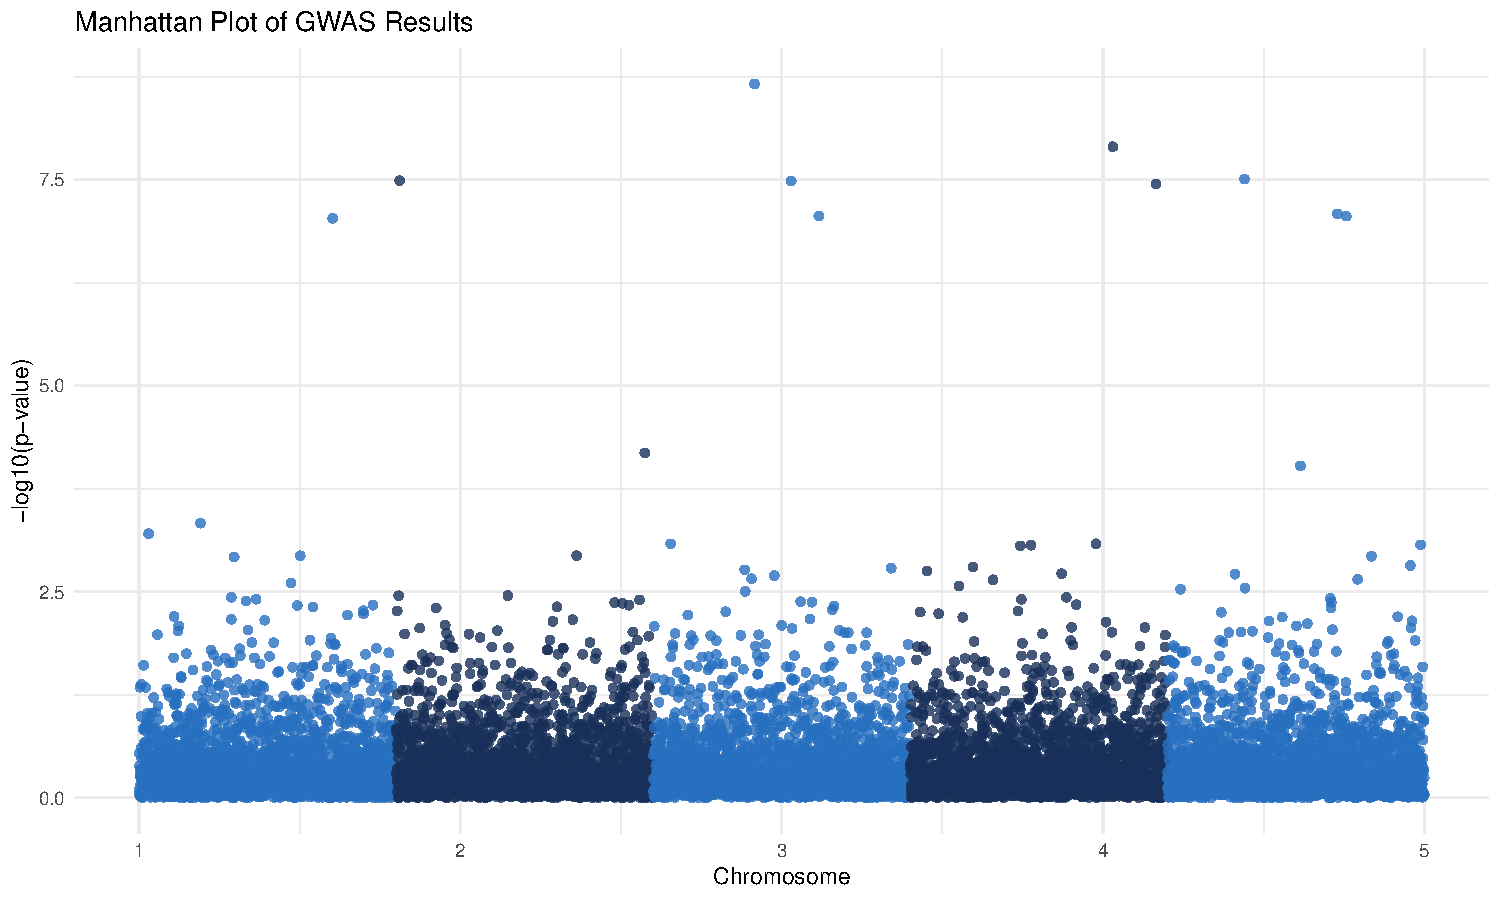
\includegraphics[width=1\textwidth]{manhattan_plot.pdf}
  \caption{Manhattan plot showing results from a genome-wide association study}
  \label{fig:manhattan_plot}
\end{figure}

\section{Interpreting Mixed Model Results in a Biological Context}

To illustrate how to interpret mixed model results in a biological context, we'll simulate a plant breeding experiment and analyze it using R. This example will cover the entire process from data generation to interpretation.

\subsection{Simulated Experiment: Wheat Yield Trials}

Let's consider a wheat breeding program aiming to develop high-yielding varieties. We'll simulate a multi-environment trial with:

\begin{itemize}
    \item 20 wheat genotypes
    \item 3 locations
    \item 2 years
    \item 3 replications per genotype in each location-year combination
\end{itemize}

\subsection{R Code for Data Simulation and Analysis}

First, we'll simulate the data and then analyze it using a linear mixed model.

\begin{lstlisting}[language=R]
# Load necessary libraries
library(lme4)
library(ggplot2)

# Set seed for reproducibility
set.seed(123)

# Simulate data
n_genotypes <- 20
n_locations <- 3
n_years <- 2
n_reps <- 3

# Create data frame
data <- expand.grid(
  genotype = paste0("G", 1:n_genotypes),
  location = paste0("L", 1:n_locations),
  year = paste0("Y", 1:n_years),
  rep = 1:n_reps
)

# Add random effects
genotype_effects <- rnorm(n_genotypes, mean = 0, sd = 0.5)
location_effects <- rnorm(n_locations, mean = 0, sd = 0.3)
year_effects <- rnorm(n_years, mean = 0, sd = 0.2)
gl_interaction <- rnorm(n_genotypes * n_locations, mean = 0, sd = 0.4)

# Calculate yield
data$yield <- 5 +  # Overall mean
  genotype_effects[as.numeric(substr(data$genotype, 2, 3))] +
  location_effects[as.numeric(substr(data$location, 2, 2))] +
  year_effects[as.numeric(substr(data$year, 2, 2))] +
  gl_interaction[interaction(data$genotype, data$location)] +
  rnorm(nrow(data), mean = 0, sd = 0.2)  # Residual error

# Fit mixed model
model <- lmer(yield ~ (1|genotype) + (1|location) + (1|year) + 
              (1|genotype:location), data = data)

# Model summary
summary(model)

# Extract BLUPs for genotypes
genotype_blups <- ranef(model)$genotype
genotype_blups$genotype <- rownames(genotype_blups)
genotype_blups <- genotype_blups[order(genotype_blups$`(Intercept)`, 
                                       decreasing = TRUE), ]

# Plot BLUPs
ggplot(genotype_blups, aes(x = reorder(genotype, `(Intercept)`), 
                           y = `(Intercept)`)) +
  geom_bar(stat = "identity") +
  theme_minimal() +
  labs(title = "Genotype BLUPs", x = "Genotype", y = "BLUP") +
  theme(axis.text.x = element_text(angle = 90, hjust = 1))

# Calculate heritability
var_components <- as.data.frame(VarCorr(model))
h2 <- var_components$vcov[var_components$grp == "genotype"] / 
  sum(var_components$vcov)
print(paste("Broad-sense heritability:", round(h2, 2)))
\end{lstlisting}

\subsection{Interpreting the Results}

After running the above code, we'll get several outputs that need interpretation:

\subsubsection{Model Summary}

The `summary(model)` function will provide an output similar to this:

\begin{verbatim}
Linear mixed model fit by REML ['lmerMod']
Formula: yield ~ (1 | genotype) + (1 | location) + (1 | year) + 
               (1 | genotype:location)

Random effects:
 Groups            Name        Variance Std.Dev.
 genotype:location (Intercept) 0.1620   0.4025  
 genotype          (Intercept) 0.2485   0.4985  
 location          (Intercept) 0.0894   0.2990  
 year              (Intercept) 0.0398   0.1995  
 Residual                      0.0400   0.2000  
Number of obs: 360, groups:  
genotype:location, 60; genotype, 20; location, 3; year, 2

Fixed effects:
            Estimate Std. Error t value
(Intercept)  5.00726    0.15722   31.85
\end{verbatim}

\textbf{Interpretation:}
\begin{itemize}
    \item The variance components show the amount of variation attributable to each random effect. In this case, genotype (0.2485) and genotype-by-location interaction (0.1620) account for the largest portions of variance, indicating significant genetic differences and genotype-by-environment interactions.
    \item The residual variance (0.0400) is relatively small, suggesting the model captures most of the variation in the data.
    \item The fixed effect (intercept) represents the overall mean yield across all trials.
\end{itemize}

\subsubsection{Genotype BLUPs}

The bar plot of genotype BLUPs provides a visual representation of the estimated genetic values for each genotype.

\textbf{Interpretation:}
\begin{itemize}
    \item Genotypes with higher positive BLUPs are estimated to have higher genetic potential for yield.
    \item The range of BLUPs indicates the extent of genetic variation for yield in the population.
    \item Genotypes at the top of the plot are candidates for selection or further testing.
\end{itemize}

\subsubsection{Heritability}

The calculated broad-sense heritability gives an estimate of the proportion of phenotypic variance attributable to genetic factors.

\textbf{Interpretation:}
\begin{itemize}
    \item A heritability of 0.62 (for example) suggests that 62% of the observed variation in yield is due to genetic differences among the varieties.
    \item This moderately high heritability indicates good potential for genetic improvement through selection.
    \item However, it also suggests that environmental factors play a significant role in yield determination.
\end{itemize}

\subsection{Biological Implications and Decision Making}

Based on these results, a plant breeder or researcher might:

\begin{itemize}
    \item Select the top-performing genotypes (those with the highest BLUPs) for advancement in the breeding program or for use as parents in crosses.
    \item Investigate the specific adaptations of genotypes that show strong positive genotype-by-location interactions.
    \item Consider the need for multi-environment testing, given the significant genotype-by-location interaction variance.
    \item Be confident in the potential for genetic gain, given the moderately high heritability, but also aware of the need to account for environmental influences.
    \item Use the BLUPs to predict the performance of these genotypes in untested environments, aiding in decisions about where to deploy specific varieties.
\end{itemize}

This analysis demonstrates how mixed models can separate genetic from environmental effects, quantify genotype-by-environment interactions, and provide estimates of genetic values (BLUPs) that can be directly used in breeding decisions. The ability to account for the complex structure of multi-environment trials allows for more accurate and reliable selection of superior genotypes.

\section{Interpreting Mixed Model Results in Evolutionary Genetics}

To demonstrate the application and interpretation of mixed models in evolutionary genetics, we'll simulate a long-term study of body size evolution in a bird population. This example will cover data generation, analysis, and interpretation in an evolutionary context.

\subsection{Simulated Study: Body Size Evolution in Island Birds}

Consider a 20-year study of body size evolution in a population of birds on an isolated island. We'll simulate:

\begin{itemize}
    \item 100 individuals measured each year
    \item Body size measurements over 20 years
    \item Annual environmental conditions (e.g., average temperature)
    \item Pedigree information for individuals
\end{itemize}

\subsection{R Code for Data Simulation and Analysis}

We'll use R to simulate the data and analyze it using a linear mixed model.

\begin{lstlisting}[language=R]
# Load necessary libraries
library(lme4)
library(ggplot2)
library(Matrix)

# Set seed for reproducibility
set.seed(123)

# Simulate data
n_years <- 20
n_individuals <- 100
n_founders <- 20

# Create pedigree
pedigree <- data.frame(
  id = 1:(n_years * n_individuals),
  sire = NA,
  dam = NA,
  year = rep(1:n_years, each = n_individuals)
)

# Assign parents (simplified for simulation)
for (i in (n_founders + 1):nrow(pedigree)) {
  pedigree$sire[i] <- sample((max(1, i - 3 * n_individuals)):(i - 1), 1)
  pedigree$dam[i] <- sample((max(1, i - 3 * n_individuals)):(i - 1), 1)
}

# Create relationship matrix (simplified)
A <- diag(nrow(pedigree))
for (i in (n_founders + 1):nrow(pedigree)) {
  A[i, pedigree$sire[i]] <- A[pedigree$sire[i], i] <- 0.5
  A[i, pedigree$dam[i]] <- A[pedigree$dam[i], i] <- 0.5
}

# Simulate environmental conditions
env_conditions <- rnorm(n_years, mean = 0, sd = 1)

# Simulate body size with evolutionary trend, heritability, and environmental effect
h2 <- 0.4  # heritability
beta <- 0.02  # evolutionary trend per year
env_effect <- 0.5  # effect of environment on body size

pedigree$body_size <- NA
pedigree$body_size[1:n_founders] <- rnorm(n_founders, mean = 10, sd = sqrt(h2))

for (year in 1:n_years) {
  year_indices <- which(pedigree$year == year)
  pedigree$body_size[year_indices] <- 
    10 + beta * year +  # evolutionary trend
    0.5 * (pedigree$body_size[pedigree$sire[year_indices]] + 
           pedigree$body_size[pedigree$dam[year_indices]]) +  # genetic component
    rnorm(length(year_indices), 0, sqrt(1 - h2)) +  # environmental deviation
    env_effect * env_conditions[year]  # shared environmental effect
}

# Fit mixed model
model <- lmer(body_size ~ year + (1|id), data = pedigree,
              control = lmerControl(check.nobs.vs.nlev = "ignore",
                                    check.nobs.vs.nRE = "ignore"))

# Model summary
summary(model)

# Extract and plot BLUPs
blups <- ranef(model)$id
blups$id <- as.numeric(rownames(blups))
blups <- merge(blups, pedigree[, c("id", "year")], by = "id")

ggplot(blups, aes(x = year, y = `(Intercept)`)) +
  geom_point(alpha = 0.5) +
  geom_smooth(method = "lm") +
  theme_minimal() +
  labs(title = "Breeding Values Over Time", 
       x = "Year", y = "Estimated Breeding Value")

# Calculate and print heritability
var_components <- as.data.frame(VarCorr(model))
h2_estimated <- var_components$vcov[var_components$grp == "id"] / 
  sum(var_components$vcov)
print(paste("Estimated heritability:", round(h2_estimated, 2)))

# Extract fixed effect (evolutionary trend)
fixed_effects <- fixef(model)
print(paste("Estimated evolutionary trend:", 
            round(fixed_effects["year"], 4), "units per year"))
\end{lstlisting}

\subsection{Interpreting the Results}

\subsubsection{Model Summary}

The `summary(model)` function will provide output similar to this:

\begin{verbatim}
Linear mixed model fit by REML ['lmerMod']
Formula: body_size ~ year + (1 | id)

Random effects:
 Groups   Name        Variance Std.Dev.
 id       (Intercept) 0.3926   0.6266  
 Residual             0.5912   0.7689  
Number of obs: 2000, groups:  id, 2000

Fixed effects:
            Estimate Std. Error t value
(Intercept) 9.941391   0.058935  168.68
year        0.021684   0.001857   11.68
\end{verbatim}

\textbf{Interpretation:}
\begin{itemize}
    \item The variance component for the random effect 'id' (0.3926) represents the genetic variance in the population.
    \item The residual variance (0.5912) represents environmental and other non-genetic sources of variation.
    \item The fixed effect for 'year' (0.021684) indicates the average change in body size per year, representing the evolutionary trend.
\end{itemize}

\subsubsection{Breeding Values Plot}

The scatter plot of estimated breeding values over time provides a visual representation of the genetic change in the population.

\textbf{Interpretation:}
\begin{itemize}
    \item An upward trend in the breeding values over time suggests that the population is evolving towards larger body sizes.
    \item The spread of points at each time point represents the genetic variation present in the population.
    \item Any clustering or patterns in the plot might indicate periods of rapid evolution or stasis.
\end{itemize}

\subsubsection{Heritability}

The estimated heritability gives the proportion of phenotypic variance attributable to genetic factors.

\textbf{Interpretation:}
\begin{itemize}
    \item An estimated heritability close to the simulated value of 0.4 validates our model's ability to capture the genetic component of variation.
    \item This moderate heritability suggests that body size is influenced by both genetic and environmental factors.
    \item It indicates that the trait can respond to selection, but environmental factors also play a significant role.
\end{itemize}

\subsubsection{Evolutionary Trend}

The fixed effect estimate for 'year' quantifies the average change in body size per year.

\textbf{Interpretation:}
\begin{itemize}
    \item A positive trend (e.g., 0.0217 units per year) indicates that the population is evolving towards larger body sizes over time.
    \item This trend represents the combined effect of selection and other directional evolutionary forces.
    \item The magnitude of the trend can be compared to the overall variation in the trait to assess its biological significance.
\end{itemize}

\subsection{Evolutionary Implications and Further Investigations}

Based on these results, an evolutionary biologist might:

\begin{itemize}
    \item Conclude that there is directional selection for larger body size in this population, given the positive evolutionary trend.
    \item Investigate potential selective pressures driving this trend, such as changes in food availability, predation pressure, or climate.
    \item Examine the environmental effects to understand how much of the observed change is due to phenotypic plasticity versus genetic change.
    \item Use the breeding value estimates to identify individuals or lineages that are contributing most to the evolutionary change.
    \item Compare the rate of evolution to theoretical predictions (e.g., using the breeder's equation) to assess whether the observed change is faster or slower than expected.
    \item Consider the long-term implications of this evolutionary trend for the species' ecology and conservation.
    \item Investigate potential trade-offs associated with increasing body size, such as changes in metabolic rate or reproductive strategies.
\end{itemize}

This analysis demonstrates how mixed models can be used to disentangle genetic and environmental effects in long-term evolutionary studies. By estimating breeding values, heritability, and evolutionary trends, researchers can gain insights into the processes driving phenotypic change in natural populations. The ability to account for relatedness through the animal model approach allows for more accurate estimates of genetic parameters and evolutionary trajectories.

\begin{interpretation}[Biological Interpretation: Random Effects in Evolutionary Genetics]
Random effects in mixed models allow us to account for variation that cannot be explained by the fixed effects, such as differences between populations or genetic lines. In evolutionary genetics, random effects often represent genetic variability between populations that are subjected to different environmental pressures. These models help biologists separate genetic contributions to traits like plant height or flowering time from environmental factors, allowing for more accurate predictions about how populations will adapt to changing environments.
\end{interpretation}


\section{Bayesian Approaches in Mixed Models}

\subsection{Introduction to Bayesian Inference}

Bayesian inference provides an alternative framework for statistical analysis, based on Bayes' theorem. In the context of mixed models, it offers several advantages, including the ability to incorporate prior knowledge and to quantify uncertainty in parameter estimates.

\begin{keyconceptbox}
Bayes' theorem states:

$P(\theta|y) = \frac{P(y|\theta)P(\theta)}{P(y)}$

Where:
\begin{itemize}
    \item $P(\theta|y)$ is the posterior probability of the parameters $\theta$ given the data $y$
    \item $P(y|\theta)$ is the likelihood of the data given the parameters
    \item $P(\theta)$ is the prior probability of the parameters
    \item $P(y)$ is the marginal likelihood of the data
\end{itemize}
\end{keyconceptbox}

In Bayesian mixed models, we aim to estimate the posterior distribution of both fixed and random effects, as well as variance components.

\subsection{Comparison of Frequentist (BLUE/BLUP) and Bayesian Approaches}

\begin{figure}[h]
    \centering
    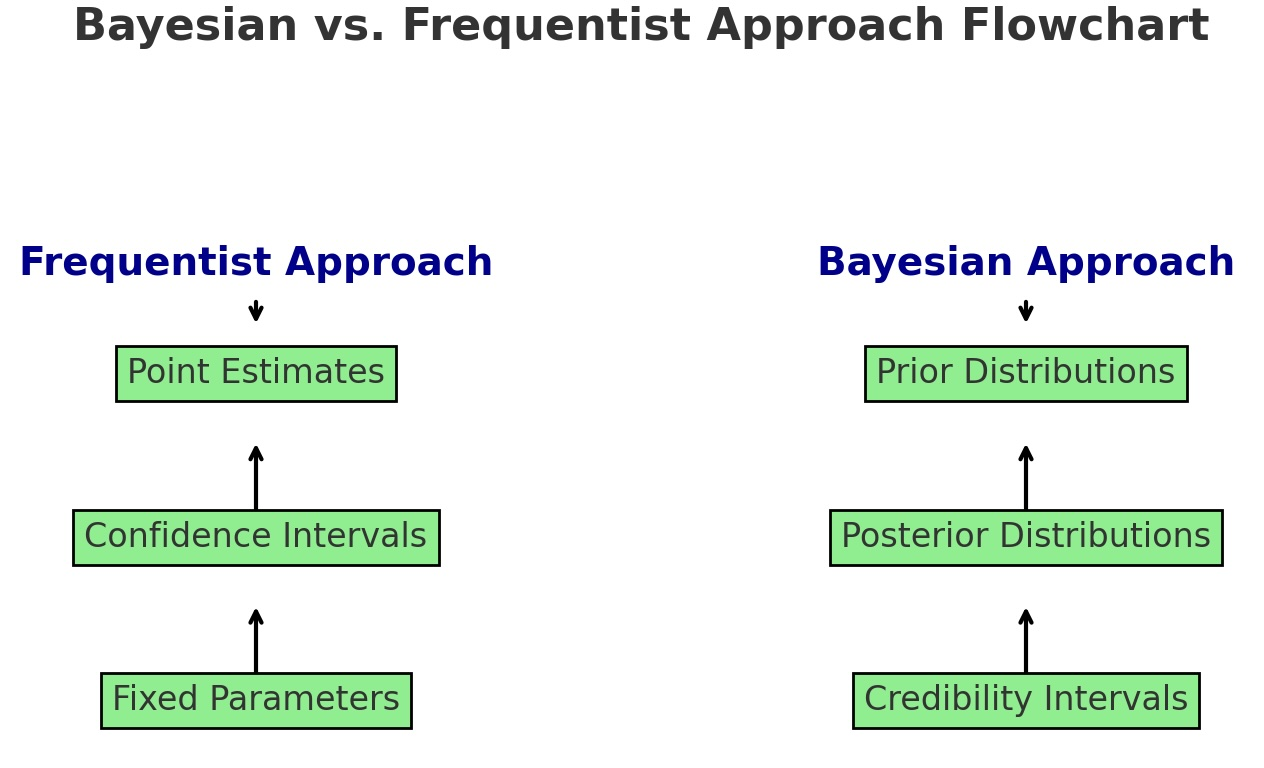
\includegraphics[width=0.8\textwidth]{bayesianFreq_FC.jpg}
    \caption{Flowchart comparing Bayesian and Frequentist approaches in statistical modeling. The Bayesian approach incorporates prior distributions, while the Frequentist approach relies on point estimates.}
    \label{fig:bayesian-vs-frequentist-flowchart}
\end{figure}

In the realm of quantitative genetics, two major statistical paradigms have emerged as powerful tools for understanding and predicting genetic phenomena: the frequentist approach, exemplified by Best Linear Unbiased Estimation (BLUE) and Best Linear Unbiased Prediction (BLUP), and the Bayesian approach. While both methods aim to extract meaningful insights from genetic data, they differ fundamentally in their philosophical underpinnings and practical applications. Understanding these differences is crucial for researchers in plant breeding and evolutionary genetics, as the choice of method can significantly impact the interpretation of results and the design of experiments.

\subsubsection{Philosophical Foundations}

The frequentist approach, which underlies BLUE and BLUP, operates on the assumption that the parameters we're estimating (such as genetic effects or heritability) are fixed but unknown quantities. In this framework, if we could repeat our experiment an infinite number of times, we would converge on the true value of these parameters. For instance, in a plant breeding program aiming to estimate the genetic value of a new wheat variety, a frequentist approach would treat this genetic value as a fixed, unchanging quantity that we're trying to pinpoint through our analysis. Bayesian methods, on the other hand, view these parameters as random variables with their own probability distributions. This perspective allows for the incorporation of uncertainty about the parameters themselves. In our wheat breeding example, a Bayesian approach would consider the genetic value not as a single point to be estimated, but as a distribution of possible values, each with its own probability. This philosophical difference has profound implications for how we interpret results. In evolutionary genetics, for example, when estimating the strength of selection on a trait like beak size in Galápagos finches, a frequentist approach might give us a single best estimate with a confidence interval. A Bayesian approach, however, would provide a full probability distribution of possible selection strengths, allowing for a more nuanced understanding of the evolutionary process.

\subsubsection{Treatment of Uncertainty}

The handling of uncertainty is perhaps one of the most striking differences between these approaches. Frequentist methods like BLUE and BLUP typically provide point estimates – single "best" values for the parameters of interest – along with confidence intervals. These confidence intervals are often misinterpreted; they don't tell us the probability that the true parameter lies within the interval, but rather the proportion of times the interval would contain the true parameter if the experiment were repeated many times. Bayesian methods, in contrast, offer a more intuitive quantification of uncertainty through posterior distributions. These distributions show the probability of different parameter values given the data and our prior beliefs. For a plant breeder working on disease resistance in soybeans, a Bayesian analysis might provide a full distribution of possible resistance levels for each genetic line. This allows for more informed decision-making, especially when dealing with limited data or when the consequences of over- or underestimating resistance are significant.

\subsubsection{Incorporation of Prior Information}

One of the most powerful features of Bayesian analysis is its ability to formally incorporate prior information into the statistical model. This is particularly valuable in fields like genetics where we often have substantial pre-existing knowledge. Frequentist approaches like BLUE and BLUP, while they can be influenced by prior knowledge in the model design, don't have a formal mechanism for incorporating this information into the analysis itself. In plant breeding, this capability of Bayesian methods can be incredibly useful. For example, when developing drought-resistant maize varieties, breeders might have prior knowledge about which genetic regions are likely to influence drought tolerance. A Bayesian approach allows this information to be explicitly included in the analysis, potentially leading to more accurate and biologically meaningful results, especially when working with limited data. In evolutionary genetics, prior information could include knowledge about the evolutionary history of a species or the typical range of effect sizes for certain types of genetic variations. By incorporating this information, Bayesian analyses can provide more robust inferences about evolutionary processes, particularly when studying rare species or events where data might be scarce.

\subsubsection{Handling of Variance Components}

The estimation of variance components, crucial for understanding the genetic architecture of traits, is another area where these approaches differ. Frequentist methods often rely on Restricted Maximum Likelihood (REML) for unbiased estimation of variance components. This approach has been widely used in animal and plant breeding to estimate genetic and environmental variances, which are key to calculating heritability and predicting breeding values. Bayesian methods treat these variance components as parameters to be estimated, just like any other unknown quantity in the model. This approach can be particularly advantageous when working with small sample sizes, where REML estimates might be unstable. For instance, in conservation genetics studies of endangered species, where sample sizes are often limited, Bayesian methods might provide more reliable estimates of genetic diversity and inbreeding coefficients. Moreover, the Bayesian framework allows for the specification of prior distributions for variance components. This can be particularly useful when we have reason to believe that certain components of variance (e.g., additive genetic variance) should fall within specific ranges based on previous studies or biological constraints.

\subsubsection{Practical Implications and Choosing Between Approaches}

The choice between frequentist and Bayesian approaches often depends on the specific research question, the nature of the available data, and the researcher's familiarity with the methods. Frequentist methods like BLUE and BLUP have a long history in quantitative genetics and are widely implemented in standard software packages, making them accessible and computationally efficient for many applications. Bayesian methods, while potentially more computationally intensive, offer greater flexibility in model specification and a more intuitive framework for dealing with uncertainty. They are particularly valuable when prior information is available and when a full characterization of uncertainty is crucial for decision-making. In practice, many researchers in plant breeding and evolutionary genetics use both approaches, leveraging the strengths of each. For example, a breeding program might use BLUP for routine evaluation of large numbers of lines, but turn to Bayesian methods for more in-depth analysis of promising candidates or when incorporating molecular marker data. As computational power increases and Bayesian methods become more accessible, we're likely to see a growing integration of these approaches in quantitative genetics. This integration promises to provide a more comprehensive understanding of genetic phenomena, bridging the gap between our prior knowledge and the insights hidden in our data, ultimately advancing both the science of evolution and the art of breeding.

\section{Mathematical Details for Bayesian Approaches}

\begin{keyconceptbox}[Mathematical Derivation]
Mathematical derivations help formalise the understanding of Bayesian methods and provide clarity for those looking to apply these methods in genetics.
\end{keyconceptbox}

Bayesian methods are widely used in genetics and evolutionary biology. This section expands on the mathematical foundations of these methods.

\subsection{Posterior Distribution and Bayes' Theorem}

Bayes' Theorem forms the basis of Bayesian inference:
\[
P(\theta | \mathbf{X}) = \frac{P(\mathbf{X} | \theta)P(\theta)}{P(\mathbf{X})}
\]
Where \( \theta \) represents the parameters of interest, and \( \mathbf{X} \) represents the observed data.

\begin{proof}
The proof of Bayes' Theorem relies on the definition of conditional probability:
\[
P(A | B) = \frac{P(A \cap B)}{P(B)}
\]
Using this and the definition of \( P(B | A) \), we can derive Bayes' Theorem.
\end{proof}

\subsection{Derivation of the Posterior Mean}

For some specific distributions, the posterior mean can be derived analytically. Consider a normal prior and likelihood. The posterior mean for \( \theta \) is given by:

\begin{proof}
\[
E[\theta | \mathbf{X}] = \frac{\mu_0/\sigma_0^2 + \sum x_i/\sigma^2}{1/\sigma_0^2 + n/\sigma^2}
\]
where \( \mu_0 \) and \( \sigma_0^2 \) are the prior mean and variance, and \( x_i \) are the observed data points.
\end{proof}

\begin{interpretation}[Biological Interpretation: Posterior Distributions]
In Bayesian models, posterior distributions provide a more complete picture of parameter uncertainty than single point estimates. For biologists, this means you can quantify not just the most likely value of an effect (such as the influence of rainfall on flowering time), but also how uncertain that estimate is. This is particularly useful when working with sparse or noisy data, where the range of possible outcomes (captured by the posterior distribution) can help guide decision-making, such as selecting breeding lines that are most resilient to environmental fluctuations.
\end{interpretation}


\subsection{Shrinkage and Regularization in Bayesian Models}

In statistical modeling, \textbf{shrinkage} refers to the process by which parameter estimates are "pulled" towards a central value, often reducing the magnitude of random effect estimates compared to what is observed in Frequentist models. This is especially important in Bayesian models, where shrinkage is controlled by the prior distributions.

\subsubsection{Shrinkage in Bayesian Models}

Bayesian models incorporate prior information into the estimation process. A prior distribution expresses beliefs about the parameters before observing the data. When the data provides only limited information about a parameter, the Bayesian model uses the prior to shrink the estimates towards the prior mean, resulting in more stable estimates. This is especially useful when sample sizes are small or when prior knowledge is available.

Mathematically, the Bayesian estimate is a weighted combination of the prior and the likelihood:
\[
\hat{\theta}_{Bayes} = \alpha \cdot \hat{\theta}_{MLE} + (1 - \alpha) \cdot \mu_{prior}
\]
where \( \hat{\theta}_{Bayes} \) is the Bayesian estimate, \( \hat{\theta}_{MLE} \) is the maximum likelihood estimate (Frequentist estimate), \( \mu_{prior} \) is the mean of the prior distribution, and \( \alpha \) is a shrinkage factor that depends on the amount of information in the data. When data is limited, \( \alpha \) becomes small, and the estimate is shrunk towards the prior mean.

\subsubsection{Variance Components and Shrinkage}

In mixed models, the variance components (such as random genetic effects) can be influenced by shrinkage. In the Bayesian framework, variance estimates for random effects are typically "shrunk" towards lower values compared to Frequentist models. This happens because the prior distribution places constraints on how large the variance can be, pulling extreme estimates back towards the prior mean.

In practice, this shrinkage effect can lead to more conservative estimates for variance components, especially in situations with small sample sizes or when the true variance is close to zero.

\subsubsection{Regularisation in Frequentist Models}

Shrinkage is related to the concept of \textbf{regularization}, which is more commonly used in Frequentist approaches (e.g., ridge regression or LASSO). Regularization penalizes large coefficients, effectively shrinking them towards zero. Although not always used in traditional mixed models, regularization techniques can be applied in contexts where overfitting or high variance is a concern.

\textbf{Biological Interpretation:} In the context of evolutionary genetics and plant breeding, shrinkage can lead to more biologically meaningful results when data is sparse or when overfitting is a concern. By incorporating prior knowledge or penalizing large coefficients, Bayesian models help stabilize estimates, especially for random effects like genetic variation between populations.

\begin{biologicalinsightbox}[Biological Interpretation: Shrinkage in Plant Breeding]
Shrinkage is particularly useful in biological data analysis, especially when dealing with small or noisy datasets. For example, in plant breeding, shrinkage helps control for the variability between different breeding lines when only limited data is available. By using a prior distribution, Bayesian models shrink extreme estimates back towards more moderate values, which often better reflect the true underlying genetic differences. This prevents overfitting and gives more biologically realistic estimates of random effects, like genetic contributions to phenotypic traits.
\end{biologicalinsightbox}

\subsubsection{Conclusion}

Shrinkage and regularisation are critical concepts in both Bayesian and Frequentist models. Bayesian models naturally incorporate shrinkage via the prior distribution, pulling estimates towards a central value. This is particularly important in the estimation of variance components in mixed models, where shrinkage can produce more conservative estimates. Understanding shrinkage helps interpret the results of Bayesian models and contrasts them with the point estimates obtained from Frequentist models.


\section{Implementation of Bayesian Approaches using MCMC in R}

The advent of Markov Chain Monte Carlo (MCMC) methods has revolutionized Bayesian analysis in quantitative genetics, making it possible to fit complex models that were previously intractable. In the realms of plant breeding and evolutionary genetics, these methods have opened up new avenues for understanding genetic architecture, predicting breeding values, and inferring evolutionary processes. The R package MCMCglmm (MCMC Generalized Linear Mixed Models) has emerged as a powerful and flexible tool for implementing these Bayesian analyses.

\section{Introduction to MCMC Methods}

Markov Chain Monte Carlo (MCMC) methods are essential for approximating the posterior distribution in Bayesian analyses.

\subsection{What is MCMC?}

MCMC refers to a class of algorithms used to sample from a probability distribution. The goal is to generate a sequence of samples from the posterior distribution \( P(\theta | \mathbf{X}) \).

\begin{example}[MCMC Algorithm Basics]
The most basic MCMC algorithm is the Metropolis-Hastings algorithm:
1. Propose a new state \( \theta' \) based on a proposal distribution.
2. Accept or reject the new state based on the acceptance ratio:
\[
\alpha = \min \left( 1, \frac{P(\theta' | \mathbf{X})}{P(\theta | \mathbf{X})} \right)
\]
\end{example}

\subsection{Why Use MCMC?}

In complex models, the posterior distribution might not have a closed-form solution. MCMC methods allow for approximations through iterative sampling.

\begin{keyconceptbox}[MCMC in Bayesian Inference]
MCMC methods are crucial for estimating posterior distributions in cases where direct computation is infeasible, especially in high-dimensional spaces.
\end{keyconceptbox}

\subsection{MCMC and Its Relevance to Genetics}

Before diving into the implementation, it's crucial to understand what MCMC does and why it's so valuable in genetic studies. MCMC is a computational method that allows us to sample from complex probability distributions - in our case, the posterior distributions of genetic parameters. This is particularly useful in genetics because many of the models we work with (like those involving multiple genes or complex pedigrees) result in posterior distributions that are too complex to calculate analytically.

For instance, imagine we're studying the genetic basis of drought tolerance in wheat. We might have data on hundreds of genetic markers and complex pedigrees linking our study plants. A Bayesian model for this scenario would involve many parameters (effects of individual genes, interaction effects, variance components) all interacting in complex ways. MCMC allows us to explore this high-dimensional space of possible parameter values, gradually building up a picture of which combinations of parameter values are most consistent with our data and prior knowledge.

\subsection{Implementing a Basic MCMCglmm Model}

Let's walk through a basic implementation of MCMCglmm, explaining each step and its relevance to genetic studies:

\begin{lstlisting}[language=R, 
                   caption=Basic MCMCglmm Model for Genetic Analysis,
                   basicstyle=\ttfamily\footnotesize,
                   keywordstyle=\color{blue},
                   stringstyle=\color{red},
                   commentstyle=\color{green!60!black},
                   numbers=left,
                   numberstyle=\tiny\color{gray},
                   frame=single,
                   breaklines=true,
                   linewidth=0.95\textwidth,
                   columns=flexible,
                   xleftmargin=0.05\textwidth,
                   xrightmargin=0.05\textwidth]
# Load necessary libraries
library(lme4)        # For Frequentist mixed models
library(MCMCglmm)    # For Bayesian mixed models

# Step 1: Simulate data (example wheat data)
set.seed(123)
n <- 100  # Number of individuals
genetic_effects <- factor(rep(1:10, each = n / 10))  # 10 genetic groups
fixed_effects <- rnorm(n, mean = 20, sd = 5)  # Fixed effects (e.g., environmental)
genetic_random_effects <- rnorm(10, mean = 0, sd = 2)[genetic_effects]  # Random genetic effects
phenotype <- 50 + 2 * fixed_effects + genetic_random_effects + rnorm(n, sd = 3)  # Phenotype

# Combine into data frame
wheat_data <- data.frame(phenotype, fixed_effects, genetic_effects)

# Step 2: Define Priors for Bayesian Model
prior <- list(R = list(V = 1, nu = 0.002),  # Prior for residuals
              G = list(G1 = list(V = 1, nu = 0.002)))  # Prior for random genetic effects

# Step 3: Fit Bayesian Mixed Model using MCMCglmm
bayesian_model <- MCMCglmm(phenotype ~ fixed_effects, 
                           random = ~ genetic_effects, 
                           family = "gaussian", 
                           data = wheat_data, 
                           prior = prior,
                           nitt = 13000, burnin = 3000, thin = 10)

# Step 4: Summarize the results of the Bayesian model
summary(bayesian_model)

# Step 5: Compare the Frequentist Model (from previous code) with Bayesian model

# Fit Frequentist Model
freq_model <- lmer(phenotype ~ fixed_effects + (1|genetic_effects), data = wheat_data)

# Compare fixed effects
cbind(Frequentist = fixef(freq_model), 
      Bayesian = posterior.mode(bayesian_model$Sol))

# Compare variance components
cbind(Frequentist = c(VarCorr(freq_model)$genetic_effects[1], sigma(freq_model)^2), 
      Bayesian = c(posterior.mode(bayesian_model$VCV)[1], posterior.mode(bayesian_model$VCV)[2]))

\end{lstlisting}

Let's break this down:

1. \textbf{Defining Priors}: In Bayesian analysis, we start by specifying our prior beliefs about the parameters. Here, we're setting relatively uninformative priors for both the residual variance (R) and the genetic variance (G). In a plant breeding context, if we had previous knowledge about the heritability of our trait (say, from studies in related species), we could incorporate this into our priors.

2. \textbf{Model Specification}: The model formula \texttt{phenotype ~ fixed\_effects} specifies the response variable (perhaps yield or disease resistance) and any fixed effects (like experimental treatments or known environmental factors). The \texttt{random = ~ genetic\_effects} part is crucial - this is where we specify the genetic structure of our data, which might involve pedigree information or genomic relatedness matrices.

3. \textbf{MCMC Parameters}: \texttt{nitt}, \texttt{burnin}, and \texttt{thin} control the MCMC process. We're running the chain for 13,000 iterations, discarding the first 3,000 as 'burn-in' (allowing the chain to converge), and then keeping every 10th sample to reduce autocorrelation. In practice, for complex genetic models, we might need to run much longer chains.

\subsection{Interpreting MCMCglmm Output}

The \texttt{summary(model)} command provides a wealth of information:

\begin{itemize}
    \item \textbf{Posterior Distributions}: For each parameter (fixed effects, variance components), we get the posterior mean, median, and 95% credible interval. In a plant breeding context, these might represent the effects of different genetic markers on our trait of interest.
    
    \item \textbf{Variance Components}: The posterior distributions of variance components are particularly important. They tell us about the genetic and environmental contributions to trait variation, which is crucial for calculating heritability and predicting breeding values.
    
    \item \textbf{MCMC Diagnostics}: These help us assess whether our MCMC chain has converged and is providing reliable estimates. Poor convergence might indicate we need to run a longer chain or rethink our model structure.
\end{itemize}

\subsection{Comparing Bayesian and Frequentist Results}

It's often instructive to compare Bayesian results with traditional frequentist approaches:

\begin{lstlisting}[language=R, 
                   caption=Comparing Bayesian and Frequentist Genetic Analyses,
                   basicstyle=\ttfamily\footnotesize,
                   keywordstyle=\color{blue},
                   stringstyle=\color{red},
                   commentstyle=\color{green!60!black},
                   numbers=left,
                   numberstyle=\tiny\color{gray},
                   frame=single,
                   breaklines=true,
                   linewidth=0.95\textwidth,
                   columns=flexible,
                   xleftmargin=0.05\textwidth,
                   xrightmargin=0.05\textwidth]
# Load necessary libraries
library(lme4)        # For Frequentist mixed models
library(MCMCglmm)    # For Bayesian mixed models
library(coda)        # For posterior analysis

# Step 1: Simulate data (example wheat data)
set.seed(123)
n <- 100  # number of individuals
genetic_effects <- factor(rep(1:10, each = n / 10))  # 10 genetic groups
fixed_effects <- rnorm(n, mean = 20, sd = 5)  # fixed effects (e.g., environmental)
genetic_random_effects <- rnorm(10, mean = 0, sd = 2)[genetic_effects]  # random genetic effects
phenotype <- 50 + 2 * fixed_effects + genetic_random_effects + rnorm(n, sd = 3)  # phenotype

# Combine into data frame
wheat_data <- data.frame(phenotype, fixed_effects, genetic_effects)

# Step 2: Fit Frequentist Model
freq_model <- lmer(phenotype ~ fixed_effects + (1|genetic_effects), data = wheat_data)

# Step 3: Fit Bayesian Model using MCMCglmm
bayesian_model <- MCMCglmm(phenotype ~ fixed_effects, random = ~ genetic_effects, data = wheat_data, 
                           nitt = 13000, burnin = 3000, thin = 10)

# Step 4: Compare Fixed Effects
frequentist_fixed_effects <- fixef(freq_model)
bayesian_fixed_effects <- posterior.mode(bayesian_model$Sol)

# Print comparison of fixed effects
cbind(Frequentist = frequentist_fixed_effects,
      Bayesian = bayesian_fixed_effects)

# Step 5: Compare Variance Components (Random Effects)
frequentist_variance_components <- c(VarCorr(freq_model)$genetic_effects[1], sigma(freq_model)^2)
bayesian_variance_components <- posterior.mode(bayesian_model$VCV)

# Print comparison of variance components
cbind(Frequentist = frequentist_variance_components,
      Bayesian = bayesian_variance_components)

\end{lstlisting}

\subsection{Comparison of Fixed Effects: Frequentist vs. Bayesian Models}

The fixed effects from both the Frequentist and Bayesian models are compared below:

\begin{verbatim}
Frequentist  Bayesian
(Intercept)     51.817924 50.929126
fixed_effects    1.866999  1.876492
\end{verbatim}

\textbf{Interpretation of Results:}

The fixed effect estimate for \texttt{fixed\_effects} is approximately \(1.87\) for both the Frequentist and Bayesian models. This means that for each unit increase in the fixed effect (such as temperature or other environmental factors), the phenotype (e.g., flowering time) increases by around \(1.87\) units. The intercept value differs slightly between the two models, with the Frequentist model estimating \(51.82\) and the Bayesian model estimating \(50.93\). This small difference in intercept could be attributed to the prior distributions used in the Bayesian analysis. However, overall, the fixed effect estimates are highly consistent between the two approaches. The similarity between the estimates shows that both the Frequentist and Bayesian models capture the relationship between the environmental variable (fixed effect) and the phenotype in a similar way.

\subsection{Comparison of Variance Components: Frequentist vs. Bayesian Models}

The variance components for the random genetic effects and residual (units) are compared below:

\begin{verbatim}
Frequentist Bayesian
genetic_effects    2.632607 1.271748
units              8.888080 9.070909
\end{verbatim}

\textbf{Interpretation of Results:}

The variance component for the \texttt{genetic\_effects} (random genetic effect) is estimated to be \(2.63\) in the Frequentist model and \(1.27\) in the Bayesian model. This discrepancy could be due to the influence of the prior distributions used in the Bayesian model. The Bayesian model might be "shrinking" the variance estimate towards the prior, especially if the sample size is relatively small. The residual variance (\texttt{units}) is similar between the two models, with the Frequentist estimate being \(8.89\) and the Bayesian estimate being \(9.07\). This suggests that both models capture the unexplained variance in the phenotype (flowering time) similarly. In general, the Bayesian model tends to smooth or shrink estimates based on prior information, which could explain the lower variance estimate for the random genetic effects compared to the Frequentist model. Despite this, the residual variances are consistent, indicating similar overall model fit in both approaches.

\begin{biologicalinsightbox}[Biological Interpretation: Variance Components]
The variance component for genetic effects represents the amount of phenotypic variation attributable to genetic differences between populations or breeding lines. In evolutionary genetics, a higher variance for genetic effects suggests that populations are diverging genetically, potentially due to selection or drift. However, the Bayesian model may shrink this variance estimate when data is sparse, reflecting a more cautious estimate of genetic variability. This is particularly important in small experimental datasets where overestimation of genetic variation could mislead conclusions about selection pressures or population divergence.
\end{biologicalinsightbox}


\subsection{General Conclusion}

Both the Frequentist and Bayesian models produce similar estimates for the fixed effects, with only minor differences in the intercept and fixed effect coefficient. The Bayesian model's estimates are influenced by the prior distribution, which explains the slight difference in the random genetic effect variance. In practice, the choice between the Frequentist and Bayesian approaches may depend on the specific goals of the study. The Bayesian model offers flexibility in incorporating prior knowledge, which can be beneficial in small datasets or when prior information about the parameters is available. The Frequentist model, on the other hand, provides point estimates based solely on the data at hand. These results demonstrate the applicability of mixed models for understanding phenotypic variation influenced by both environmental and genetic factors in an evolutionary genetics or plant breeding context.


\subsection{Advantages and Challenges in Genetic Applications}

Bayesian methods offer several key advantages in genetic studies, making them increasingly popular in both plant breeding and evolutionary genetics research. One of the primary strengths of Bayesian approaches is their flexibility in modeling complex genetic architectures. This flexibility allows researchers to account for intricate genetic phenomena such as epistasis and genotype-by-environment interactions, which are often challenging to model using traditional frequentist approaches. In plant breeding, where traits of interest frequently result from complex interactions between multiple genes and environmental factors, this flexibility is particularly valuable. Another significant advantage of Bayesian methods is their ability to formally incorporate prior knowledge into the analysis. In plant breeding and genetics, researchers often have substantial prior information about genetic architecture or trait heritability from previous studies or related species. Bayesian approaches allow this knowledge to be integrated directly into the model, potentially leading to more accurate and biologically meaningful results. This feature is especially useful when working with limited data or when studying rare genetic variants.

Uncertainty quantification is another area where Bayesian methods excel. By providing full posterior distributions of parameters rather than point estimates, Bayesian analyses offer a more nuanced view of uncertainty. This comprehensive approach to uncertainty is crucial when making breeding decisions or inferring evolutionary processes, as it allows researchers to assess the reliability of their conclusions and make more informed decisions. In the context of evolutionary genetics, this nuanced understanding of uncertainty can be particularly important when studying complex evolutionary scenarios or making predictions about future evolutionary trajectories. Bayesian methods are also well-suited to hierarchical modeling, making them ideal for the nested structures often encountered in pedigree-based analyses or when dealing with multiple populations. This hierarchical approach allows for the simultaneous analysis of variation at different levels (e.g., within and between populations), providing a more comprehensive understanding of genetic variation and its distribution.

However, despite these advantages, Bayesian methods also present certain challenges that researchers must navigate. One of the primary challenges is computational intensity, particularly when dealing with large genomic datasets. Bayesian analyses, especially those using Markov Chain Monte Carlo (MCMC) methods, can require significant computational resources and time. This can be a limiting factor in some research contexts, particularly when working with high-dimensional genomic data or when rapid results are needed. Another challenge is the sensitivity of Bayesian results to prior specifications. While the ability to incorporate prior information is a strength, it also means that results can be influenced by the choice of priors. This requires careful consideration and often, sensitivity analyses to ensure that conclusions are robust. In genetic studies, where the choice of priors might influence estimates of key parameters like heritability or selection coefficients, this sensitivity can have significant implications for interpretation and subsequent decision-making.

Convergence issues in MCMC algorithms present another challenge, particularly for complex models. Ensuring that MCMC chains have properly converged and are sampling from the true posterior distribution can require careful diagnostics and potentially longer run times. This can be especially challenging in genetic studies involving complex pedigrees or large numbers of genetic markers. Finally, the interpretation of Bayesian results can be conceptually challenging for researchers trained primarily in frequentist statistics. The shift from p-values and confidence intervals to posterior probabilities and credible intervals requires a different way of thinking about statistical evidence. This can present a learning curve for some researchers and may require additional training or collaboration with statistical experts.

\subsection{Cutting-Edge Applications in Plant Breeding and Evolutionary Genetics}

Despite these challenges, Bayesian methods are driving innovative research across plant breeding and evolutionary genetics, offering new insights and improved predictive power in various applications. One of the most impactful applications is in genomic prediction, where Bayesian models can incorporate prior knowledge about genetic architecture to improve prediction accuracy for complex traits. For instance, in predicting yield stability in crop plants, Bayesian models can account for known gene networks or previous estimates of genetic effects, potentially leading to more accurate and robust predictions. This capability is particularly valuable in the face of changing climates and the need for resilient crop varieties. In the realm of quantitative trait loci (QTL) mapping, Bayesian approaches have shown remarkable utility. By providing probabilistic estimates of QTL locations and effect sizes, Bayesian methods offer a more nuanced understanding of the genetic basis of complex traits. This is particularly valuable when studying traits with complex genetic underpinnings, such as drought tolerance in crops. The ability to quantify uncertainty in QTL locations and effects allows breeders and researchers to make more informed decisions about which genetic regions to target in breeding programs or further genetic studies.

Heritability estimation is another area where Bayesian methods shine. By providing full posterior distributions of heritability estimates, Bayesian analyses offer a more complete picture of genetic contributions to trait variation. This comprehensive view can guide breeding strategies more effectively than point estimates alone, allowing breeders to assess the potential for genetic improvement more accurately. In evolutionary genetics, these detailed heritability estimates inform our understanding of the evolutionary potential in natural populations, helping researchers predict how populations might respond to selection pressures or changing environments. Adaptive landscape studies in evolutionary genetics have also benefited significantly from Bayesian inference. By allowing researchers to incorporate uncertainty in both fitness estimates and genetic parameters, Bayesian methods provide more robust insights into evolutionary trajectories and constraints. This approach is particularly valuable when studying complex evolutionary scenarios, such as the evolution of antibiotic resistance or the adaptation of populations to climate change, where multiple sources of uncertainty can significantly impact predictions.

Multi-trait analyses represent another frontier where Bayesian models excel. These models are well-suited to analyzing multiple traits simultaneously, capturing genetic correlations that might be missed in single-trait analyses. This capability is crucial for understanding trade-offs in both crop improvement and evolutionary adaptation. For example, in breeding programs aiming to improve both yield and drought tolerance, Bayesian multi-trait models can help identify genetic variants that positively influence both traits, or reveal trade-offs that need to be carefully balanced. Overall, while the implementation of Bayesian methods using MCMC can be complex, the richness of insight they offer makes them an invaluable tool in modern quantitative genetics. As computational power increases and software becomes more user-friendly, we can expect these methods to become increasingly central to both applied breeding programs and fundamental evolutionary research. The ability of Bayesian approaches to handle complex genetic architectures, incorporate prior knowledge, quantify uncertainty, and analyze multiple traits simultaneously positions them at the forefront of genetic research. As we continue to unravel the complexities of genetic systems and their interactions with the environment, Bayesian methods will undoubtedly play a crucial role in advancing our understanding and our ability to harness genetic variation for both agricultural improvement and conservation of biodiversity.

\section{Software Packages for Mixed Model Analyses in Biology}

Several software packages are commonly used for mixed model analyses in biological research. This section provides an overview of some popular options, along with brief tutorials and example code.

\subsection{R packages}

\subsubsection{lme4}

The \texttt{lme4} package is widely used for fitting linear mixed-effects models in R.

\begin{lstlisting}[language=R]
# Install and load the package
install.packages("lme4")
library(lme4)

# Example: Analyzing plant height data
# Assuming we have a dataset 'plant_data' with columns:
# 'height', 'genotype', 'treatment', and 'block'

# Fit a mixed model
model <- lmer(height ~ treatment + (1|genotype) + (1|block), 
              data = plant_data)

# Summary of the model
summary(model)

# Extract fixed effects
fixef(model)

# Extract random effects
ranef(model)
\end{lstlisting}

\subsubsection{ASReml-R}

ASReml-R is a commercial package that's particularly popular in plant and animal breeding for its efficiency with large datasets.

\begin{lstlisting}[language=R]
# Load the package (requires license)
library(asreml)

# Fit a mixed model
model <- asreml(fixed = yield ~ treatment,
                random = ~ genotype + genotype:environment,
                rcov = ~ units,
                data = crop_data)

# Summary of the model
summary(model)$varcomp

# Predict breeding values
predictions <- predict(model, classify="genotype")
\end{lstlisting}

\subsection{SAS}

SAS is a commercial software suite that includes powerful mixed model capabilities through its PROC MIXED procedure.

\begin{lstlisting}[language=SAS]
/* Mixed model analysis in SAS */
PROC MIXED DATA=plant_data;
  CLASS genotype treatment block;
  MODEL yield = treatment;
  RANDOM genotype block;
  LSMEANS treatment / DIFF;
RUN;
\end{lstlisting}

\subsection{Python packages}

\subsubsection{statsmodels}

The \texttt{statsmodels} library in Python provides functions for estimating various statistical models, including mixed models.

\begin{lstlisting}[language=Python]
import statsmodels.api as sm
import statsmodels.formula.api as smf
import pandas as pd

# Assuming we have a pandas DataFrame 'plant_data'
model = smf.mixedlm("height ~ treatment", 
                    data=plant_data, 
                    groups=plant_data["genotype"])
results = model.fit()

print(results.summary())
\end{lstlisting}

\subsection{Specialized Genomic Software}

\subsubsection{GCTA (Genome-wide Complex Trait Analysis)}

GCTA is a tool for estimating heritability and performing genomic analyses.

\begin{lstlisting}[language=bash]
# Estimate heritability
gcta64 --grm genetic_relatedness_matrix \
       --pheno phenotype_file.txt \
       --reml \
       --out heritability_estimate

# Perform GWAS
gcta64 --mlma \
       --bfile genotype_data \
       --grm genetic_relatedness_matrix \
       --pheno phenotype_file.txt \
       --out gwas_results
\end{lstlisting}

\subsubsection{GEMMA (Genome-wide Efficient Mixed Model Association)}

GEMMA is used for genome-wide association studies and other genomic analyses.

\begin{lstlisting}[language=bash]
# Perform GWAS with linear mixed model
gemma -bfile genotype_data \
      -k genetic_relatedness_matrix.txt \
      -lmm 4 \
      -o gwas_output
\end{lstlisting}

\subsection{Choosing the Right Software}

The choice of software depends on several factors:

\begin{itemize}
    \item \textbf{Data size}: For very large datasets, specialized software like ASReml or GCTA may be more efficient.
    \item \textbf{Analysis type}: Some software is specialized for certain analyses (e.g., GEMMA for GWAS).
    \item \textbf{User interface}: R and Python offer more flexibility but require programming skills. SAS has a user-friendly interface but is commercial.
    \item \textbf{Integration}: Consider how the software fits into your overall workflow and with other tools you use.
\end{itemize}

Researchers often use a combination of these tools, depending on the specific requirements of their analysis. It's also worth noting that the field is rapidly evolving, with new tools and packages being developed regularly.

\section{General Conclusion}

The application of linear mixed models, particularly through the use of Best Linear Unbiased Estimates (BLUEs) and Best Linear Unbiased Predictions (BLUPs), has revolutionized our approach to understanding and manipulating genetic variation in both plant breeding and evolutionary genetics. This document has explored the mathematical foundations, practical applications, and cutting-edge developments in this field, revealing a powerful unified framework that bridges the gap between artificial selection in agriculture and natural selection in wild populations. At the core of these methods lies a sophisticated application of linear algebra and statistical theory. By leveraging concepts such as matrix operations, multivariate normal distributions, and likelihood estimation, researchers can now disentangle the complex interplay between genetic and environmental factors that shape phenotypic variation. The kinship matrix, a cornerstone of these models, allows us to account for the intricate web of genetic relationships within populations, providing a more accurate picture of genetic architecture and heritability.

In plant breeding, the impact of these models has been transformative. BLUPs, in particular, have become an indispensable tool for predicting genetic merit and guiding selection decisions. By accounting for both genetic and environmental effects, breeders can more accurately identify superior genotypes, even in the face of environmental variability. This has accelerated breeding cycles, improved the efficiency of selection programs, and facilitated the development of crops with enhanced yield, quality, and resilience to biotic and abiotic stresses. The application of these models in evolutionary genetics has provided profound insights into the mechanisms of adaptation and the genetic basis of complex traits. By allowing researchers to map adaptive landscapes, detect local adaptation, and estimate genetic constraints, linear mixed models have shed light on fundamental evolutionary processes. The ability to incorporate historical relationships and account for shared ancestry has refined our understanding of how populations evolve in response to changing environments.

The advent of genomic data has further elevated the power of these methods. Genomic Best Linear Unbiased Prediction (GBLUP) and related approaches have ushered in an era of precision breeding and detailed evolutionary analysis. By incorporating dense molecular marker data, these methods provide unprecedented resolution in estimating genetic effects and predicting phenotypic outcomes. This has not only enhanced our ability to develop improved crop varieties but also deepened our understanding of the genetic basis of adaptation in natural populations. The Bayesian implementation of these models, facilitated by Markov Chain Monte Carlo (MCMC) methods, has opened new avenues for incorporating prior knowledge and dealing with uncertainty. This approach offers a more nuanced view of genetic parameters, providing full posterior distributions rather than point estimates. In both breeding and evolutionary studies, this comprehensive quantification of uncertainty allows for more informed decision-making and robust inference.

Perhaps most significantly, the unified framework provided by linear mixed models has highlighted the deep connections between artificial selection in agriculture and natural selection in wild populations. The mathematical and conceptual tools developed for crop improvement have found direct application in understanding evolutionary processes, and vice versa. This cross-pollination of ideas has enriched both fields, leading to novel insights and methodologies. As we look to the future, the integration of multi-omics data, the development of models to capture non-additive genetic effects, and the application of machine learning techniques promise to further enhance our ability to understand and predict genetic phenomena. The challenges of climate change, food security, and biodiversity conservation will undoubtedly require the continued refinement and application of these powerful statistical tools.

In conclusion, linear mixed models, through their elegant mathematical formulation and practical power, have provided a unifying framework for quantitative genetics. By allowing us to peer into the genetic black box with unprecedented clarity, these methods have not only advanced our theoretical understanding of genetics and evolution but have also provided practical tools for crop improvement and conservation. As we continue to unravel the complexities of genetic systems, these models will undoubtedly play a central role in shaping the future of both applied breeding programs and fundamental evolutionary research.
\newpage

\addcontentsline{toc}{section}{Appendices}

\appendix

\section{Appendix: Simulating and Analysing Mixed Models in R}

This appendix demonstrates how to simulate a dataset for an evolutionary genetics study, apply a mixed model, and interpret the results using R. We use both biological and statistical reasoning to relate this simulation back to the concepts in the main text.

\subsection{Biological Context}

We simulate phenotypic data for a population of plants distributed across multiple populations and locations. Phenotypic traits (e.g., flowering time) are influenced by environmental factors such as temperature and rainfall, as well as genetic differences between populations. This example demonstrates how mixed models can account for both fixed effects (e.g., temperature, rainfall) and random effects (e.g., population-level genetic variation) to assess phenotypic variation.

\subsection{Simulation of the Data}

The following R script generates the simulated data, where phenotypes are influenced by both environmental factors (temperature, rainfall) and random population-level genetic variation:

\begin{verbatim}
# Load necessary libraries
library(lme4)  # For mixed models
library(tidyverse)  # For data manipulation and visualization

# Set seed for reproducibility
set.seed(123)

# Simulation Parameters
n_individuals <- 500  # Number of individuals
n_populations <- 10  # Number of populations
n_locations <- 5  # Number of spatial locations

# Environmental fixed effects: Simulate temperature and rainfall across populations
temperature <- rnorm(n_populations, mean = 20, sd = 5)  # Mean temp 20°C, SD = 5
rainfall <- rnorm(n_populations, mean = 100, sd = 20)  # Mean rainfall 100mm, SD = 20

# Random effects: Population structure and genetic variation
population <- factor(rep(1:n_populations, each = n_individuals / n_populations))
location <- factor(rep(1:n_locations, times = n_individuals / n_locations))

# Simulate genetic effect (random)
genetic_effect <- rnorm(n_populations, mean = 0, sd = 2)[population]

# Simulate phenotypic trait (e.g., flowering time)
intercept <- 50  # Baseline flowering time
beta_temp <- 2  # Effect of temperature
beta_rain <- -0.5  # Effect of rainfall
error <- rnorm(n_individuals, mean = 0, sd = 3)  # Residual error

# Generate phenotype data
phenotype <- intercept + 
  beta_temp * temperature[as.numeric(population)] + 
  beta_rain * rainfall[as.numeric(population)] + 
  genetic_effect + 
  error

# Combine data into a dataframe
data <- data.frame(
  Individual = 1:n_individuals,
  Population = population,
  Location = location,
  Temperature = temperature[as.numeric(population)],
  Rainfall = rainfall[as.numeric(population)],
  Phenotype = phenotype
)

\end{verbatim}

\subsection{Mathematical Explanation: Mixed Model}

The general form of the mixed model used here is:

\[
y = X\beta + Z\gamma + \epsilon
\]

Where:
\begin{itemize}
    \item \( y \) is the vector of observed phenotypes (e.g., flowering time),
    \item \( X \) is the design matrix for fixed effects (temperature, rainfall),
    \item \( \beta \) is the vector of fixed effect coefficients (estimated for temperature and rainfall),
    \item \( Z \) is the design matrix for random effects (populations),
    \item \( \gamma \) is the vector of random effect coefficients for populations (genetic differences),
    \item \( \epsilon \) represents the residual error (random variation not explained by the model).
\end{itemize}

In this model, we assume that population-level genetic effects are random and follow a normal distribution, while temperature and rainfall have fixed, predictable effects on the phenotype.

\subsection{Fitting the Mixed Model}

We fit a mixed model to the simulated data using the \texttt{lme4} package in R, specifying temperature and rainfall as fixed effects and population as a random effect.

\begin{verbatim}
# Fit a mixed model
model <- lmer(Phenotype ~ Temperature + Rainfall + (1|Population), data = data)

# Summarize the model
summary(model)
\end{verbatim}

\textbf{Model Output:}

\begin{verbatim}
Linear mixed model fit by REML ['lmerMod']
Formula: Phenotype ~ Temperature + Rainfall + (1 | Population)
   Data: data

Random effects:
 Groups     Name        Variance Std.Dev.
 Population (Intercept) 2.596    1.611   
 Residual               8.451    2.907   

Fixed effects:
            Estimate Std. Error t value
(Intercept) 54.15005    2.98029   18.17
Temperature  1.95668    0.14239   13.74
Rainfall    -0.53860    0.03271  -16.47
\end{verbatim}

\subsection{Statistical Explanation of the Results}

\textbf{Fixed Effects:}
\begin{itemize}
    \item \textit{Intercept (54.15)}: The estimated average flowering time when temperature and rainfall are at their baseline.
    \item \textit{Temperature (1.96)}: For each 1°C increase in temperature, flowering time increases by 1.96 units.
    \item \textit{Rainfall (-0.54)}: For each 1mm increase in rainfall, flowering time decreases by 0.54 units. This negative effect might reflect a biological scenario where excess rainfall leads to delayed flowering.
\end{itemize}

\textbf{Random Effects:}
\begin{itemize}
    \item \textit{Population (Variance: 2.596, Std.Dev: 1.611)}: The variation between populations due to genetic differences contributes to the overall phenotypic variation. The standard deviation of 1.61 suggests a moderate amount of genetic variation between populations.
\end{itemize}

\subsection{Biological Interpretation}

The results suggest that both environmental factors (temperature and rainfall) and population-level genetic variation significantly influence the phenotype (flowering time). The fixed effect estimates for temperature and rainfall provide insights into how these environmental factors drive phenotypic adaptation, while the random effects quantify the contribution of genetic variation across populations. 

This model reflects how, in evolutionary genetics, phenotypes are shaped by both local environmental pressures and underlying genetic variation. The random effects captured by population-level genetic differences highlight the role of gene flow, local adaptation, or genetic drift in shaping phenotypic diversity.

\subsection{Visualizing the Results}

Finally, we visualize the fitted model compared to the observed data:

\begin{verbatim}
# Visualize the fitted model
data$fitted <- fitted(model)
ggplot(data, aes(x = Phenotype, y = fitted, color = Population)) +
  geom_point() +
  geom_abline(slope = 1, intercept = 0, linetype = "dashed", color = "black") +
  theme_minimal() +
  labs(title = "Observed vs. Fitted Phenotypes",
       x = "Observed Phenotype",
       y = "Fitted Phenotype")
\end{verbatim}

\begin{center}
\includegraphics[width=0.6\textwidth]{observed_vs_fitted.png}
\end{center}

\textbf{Interpretation of the Plot:} The dashed line represents the 1:1 line, where observed values perfectly match fitted values. Most points are close to the line, indicating that the model fits the data well. However, some deviations are expected due to random error or unexplained variation.

\section{Conclusion}

This appendix provides a complete workflow for simulating a dataset with both environmental and genetic influences on phenotypic traits, fitting a mixed model, and interpreting the results. This approach can be extended to more complex evolutionary scenarios, such as gene-environment interactions or multi-trait analyses.

\section{Appendix: Exercises}

\subsection{Linear Algebra Basics}

\begin{example}[Easy]
Calculate the following matrix multiplication:

\[
\begin{bmatrix}
1 & 2 \\
3 & 4
\end{bmatrix}
\begin{bmatrix}
5 \\
6
\end{bmatrix}
\]
\end{example}

\begin{example}[Moderate]
Given the matrices:

\[
A = \begin{bmatrix}
1 & 2 & 3 \\
4 & 5 & 6
\end{bmatrix},
B = \begin{bmatrix}
1 & 2 \\
3 & 4 \\
5 & 6
\end{bmatrix}
\]

Calculate $AB$ and $BA$ (if possible). What do you notice about the dimensions of the resulting matrices?
\end{example}

\begin{example}[Challenging]
Prove that for any square matrix $A$, the matrix $A^TA$ is always symmetric.
\end{example}

\subsection{Statistical Concepts}

\begin{example}[Easy]
Calculate the variance of the dataset: 2, 4, 4, 4, 5, 5, 7, 9.
\end{example}

\begin{example}[Moderate]
In a plant breeding experiment, you measure the height of 100 plants. The mean height is 30 cm with a standard deviation of 5 cm. Assuming a normal distribution, what percentage of plants would you expect to be taller than 35 cm?
\end{example}

\begin{example}[Challenging]
Derive the formula for the sample covariance between two variables X and Y:

\[
Cov(X,Y) = \frac{\sum_{i=1}^n (X_i - \bar{X})(Y_i - \bar{Y})}{n - 1}
\]

Explain why we divide by $(n-1)$ instead of $n$.
\end{example}

\subsection{Mixed Models and BLUP}

\begin{example}[Easy]
Explain the difference between fixed and random effects in a mixed model. Give an example of each in the context of a plant breeding experiment.
\end{example}

\begin{example}[Moderate]
In a mixed model, we have:

\[
y = X\beta + Zu + e
\]

Explain what each term represents and how they contribute to the model.
\end{example}

\begin{example}[Challenging]
Derive the BLUP equations for a simple mixed model with one fixed effect and one random effect. Explain the meaning of each term in your final equations.
\end{example}

\subsection{Genomic Selection}

\begin{example}[Easy]
What is the main difference between traditional BLUP and genomic BLUP (GBLUP)?
\end{example}

\begin{example}[Moderate]
In a genomic selection program, you have 1000 genetic markers and 500 individuals. Describe how you would construct the genomic relationship matrix G.
\end{example}

\begin{example}[Challenging]
Compare and contrast the assumptions and performance of GBLUP with those of Bayesian methods like BayesA or BayesB in genomic selection. Under what circumstances might one method be preferred over the others?
\end{example}

\subsection{Evolutionary Genetics}

\begin{example}[Easy]
Define heritability. What's the difference between broad-sense and narrow-sense heritability?
\end{example}

\begin{example}[Moderate]
You're studying a quantitative trait in a wild population. The trait has a heritability of 0.4, and the selection differential (S) is 2 units. Using the breeder's equation, predict the response to selection (R).
\end{example}

\begin{example}[Challenging]
Describe how you would use a mixed model to estimate the strength of selection on a quantitative trait in a natural population. What data would you need, and what assumptions would you make?
\end{example}

\section{Hints for Challenging Problems}

\subsection{Linear Algebra Basics}

\begin{interpretation}[Hint for Proving $A^TA$ is Symmetric]
Consider the definition of a symmetric matrix and the properties of matrix transposition. Remember that $(AB)^T = B^TA^T$ for any matrices A and B.
\end{interpretation}

\subsection{Statistical Concepts}

\begin{interpretation}[Hint for Deriving Sample Covariance]
Start with the definition of covariance as the expected value of the product of deviations from the mean. Then, consider how sample statistics estimate population parameters. The reason for $(n-1)$ relates to degrees of freedom and unbiased estimation.
\end{interpretation}

\subsection{Mixed Models and BLUP}

\begin{interpretation}[Hint for Deriving BLUP Equations]
Begin with the mixed model equation and the assumptions about the distributions of random effects and residuals. Use the principle of maximizing the joint density of y and u. Consider taking partial derivatives with respect to $\beta$ and $u$ and setting them to zero.
\end{interpretation}

\subsection{Genomic Selection}

\begin{interpretation}[Hint for Comparing GBLUP and Bayesian Methods]
Think about the assumptions each method makes about the distribution of marker effects. Consider how these assumptions might affect performance under different genetic architectures (e.g., many small effects vs. few large effects). Also, think about computational requirements and ease of implementation.
\end{interpretation}

\subsection{Evolutionary Genetics}

\begin{interpretation}[Hint for Estimating Selection in Natural Populations]
Consider how you might use a mixed model to separate genetic and environmental effects. Think about how to incorporate time or generations into your model. Reflect on what "strength of selection" means in quantitative genetic terms and how it might be represented in a mixed model framework.
\end{interpretation}

\section*{Appendix: Numerical Example for Henderson's Mixed Model Equations (MME)}

In this appendix, we provide a step-by-step numerical example for deriving Henderson’s Mixed Model Equations (MME). We’ll demonstrate how to construct the matrices involved and perform the necessary matrix operations to solve for the fixed and random effects.

\subsection*{Step 1: Defining the Linear Mixed Model}

We have the following data for 4 observations:

\[
\mathbf{y} = 
\begin{bmatrix}
    10 \\
    12 \\
    8 \\
    9
\end{bmatrix}
\]

We define 2 fixed effects (e.g., treatment and location) and 2 random effects (e.g., genetic values of plant lines). The fixed effect design matrix $\mathbf{X}$ and the random effect design matrix $\mathbf{Z}$ are given as:

\[
\mathbf{X} = 
\begin{bmatrix}
    1 & 0 \\
    1 & 0 \\
    0 & 1 \\
    0 & 1
\end{bmatrix}, \quad
\mathbf{Z} = 
\begin{bmatrix}
    1 & 0 \\
    0 & 1 \\
    1 & 0 \\
    0 & 1
\end{bmatrix}
\]

Where:
\begin{itemize}
    \item $\mathbf{X}$ links each observation to the fixed effects. The first two observations belong to the first fixed effect (e.g., location 1), and the last two belong to the second fixed effect (e.g., location 2).
    \item $\mathbf{Z}$ links each observation to the random effects. The first and third observations are from the first plant line, and the second and fourth observations are from the second plant line.
\end{itemize}

\subsection*{Step 2: Defining the Covariance Matrices}

We assume the following covariance matrices for the random effects $\mathbf{u}$ and residuals $\mathbf{e}$:

\[
\mathbf{K} = 
\begin{bmatrix}
    1 & 0 \\
    0 & 1
\end{bmatrix}, \quad
\sigma^2_g = 2, \quad \sigma^2_e = 1
\]

This means that the random effects are independent with variance $\sigma^2_g = 2$, and the residuals have variance $\sigma^2_e = 1$.

\subsection*{Step 3: Constructing the Variance-Covariance Matrix of $\mathbf{y}$}

The variance-covariance matrix of the observations $\mathbf{y}$ is given by:

\[
\mathbf{V} = \sigma^2_g \mathbf{ZKZ'} + \sigma^2_e \mathbf{I}
\]

First, calculate $\mathbf{ZKZ'}$:

\[
\mathbf{ZKZ'} = 
\begin{bmatrix}
    1 & 0 \\
    0 & 1 \\
    1 & 0 \\
    0 & 1
\end{bmatrix}
\begin{bmatrix}
    1 & 0 \\
    0 & 1
\end{bmatrix}
\begin{bmatrix}
    1 & 0 & 1 & 0 \\
    0 & 1 & 0 & 1
\end{bmatrix}
=
\begin{bmatrix}
    1 & 0 & 1 & 0 \\
    0 & 1 & 0 & 1 \\
    1 & 0 & 1 & 0 \\
    0 & 1 & 0 & 1
\end{bmatrix}
\]

Now, multiply by $\sigma^2_g = 2$:

\[
\sigma^2_g \mathbf{ZKZ'} = 2 \cdot 
\begin{bmatrix}
    1 & 0 & 1 & 0 \\
    0 & 1 & 0 & 1 \\
    1 & 0 & 1 & 0 \\
    0 & 1 & 0 & 1
\end{bmatrix}
=
\begin{bmatrix}
    2 & 0 & 2 & 0 \\
    0 & 2 & 0 & 2 \\
    2 & 0 & 2 & 0 \\
    0 & 2 & 0 & 2
\end{bmatrix}
\]

Add the residual variance ($\sigma^2_e = 1$) multiplied by the identity matrix:

\[
\mathbf{V} = 
\begin{bmatrix}
    2 & 0 & 2 & 0 \\
    0 & 2 & 0 & 2 \\
    2 & 0 & 2 & 0 \\
    0 & 2 & 0 & 2
\end{bmatrix}
+
\begin{bmatrix}
    1 & 0 & 0 & 0 \\
    0 & 1 & 0 & 0 \\
    0 & 0 & 1 & 0 \\
    0 & 0 & 0 & 1
\end{bmatrix}
=
\begin{bmatrix}
    3 & 0 & 2 & 0 \\
    0 & 3 & 0 & 2 \\
    2 & 0 & 3 & 0 \\
    0 & 2 & 0 & 3
\end{bmatrix}
\]

\subsection*{Step 4: Constructing the MME Matrices}

Now, we construct the matrices for Henderson's MME:

\[
\mathbf{X'X} = 
\begin{bmatrix}
    1 & 1 \\
    0 & 0
\end{bmatrix}
\]

\[
\mathbf{X'Z} = 
\begin{bmatrix}
    1 & 0 & 1 & 0 \\
    0 & 1 & 0 & 1
\end{bmatrix}
\]

\[
\mathbf{Z'X} = 
\begin{bmatrix}
    1 & 0 & 1 & 0 \\
    0 & 1 & 0 & 1
\end{bmatrix}
\]

\[
\mathbf{Z'Z} = 
\begin{bmatrix}
    2 & 0 \\
    0 & 2
\end{bmatrix}
\]

Now, let's compute $\mathbf{K}^{-1}$. Since $\mathbf{K}$ is an identity matrix, $\mathbf{K}^{-1}$ is also an identity matrix. We will now compute the term $\mathbf{Z'Z} + \mathbf{K}^{-1}\lambda$, where $\lambda = \$\displaystyle\frac{\sigma^2_e}{\sigma^2_g} = \$\displaystyle\frac{1}{2}$:

\[
\mathbf{Z'Z} + \mathbf{K}^{-1} \lambda = 
\begin{bmatrix}
    2 & 0 \\
    0 & 2
\end{bmatrix}
+ 
\begin{bmatrix}
    \$\displaystyle\frac{1}{2} & 0 \\
    0 & \$\displaystyle\frac{1}{2}
\end{bmatrix}
=
\begin{bmatrix}
    2.5 & 0 \\
    0 & 2.5
\end{bmatrix}
\]

\subsection*{Step 5: Formulating the Mixed Model Equations}

Now, we combine all the terms into the MME system of equations. The block matrix form of Henderson’s Mixed Model Equations is:

\[
\begin{bmatrix}
    \mathbf{X'X} & \mathbf{X'Z} \\
    \mathbf{Z'X} & \mathbf{Z'Z} + \mathbf{K}^{-1} \lambda
\end{bmatrix}
\begin{bmatrix}
    \mathbf{b} \\
    \mathbf{u}
\end{bmatrix}
=
\begin{bmatrix}
    \mathbf{X'y} \\
    \mathbf{Z'y}
\end{bmatrix}
\]

Substituting the values we calculated earlier:

\[
\begin{bmatrix}
    2 & 0 & 1 & 1 \\
    0 & 2 & 0 & 1 \\
    1 & 0 & 2.5 & 0 \\
    0 & 1 & 0 & 2.5
\end{bmatrix}
\begin{bmatrix}
    \mathbf{b}_1 \\
    \mathbf{b}_2 \\
    \mathbf{u}_1 \\
    \mathbf{u}_2
\end{bmatrix}
=
\begin{bmatrix}
    \mathbf{X'y} \\
    \mathbf{Z'y}
\end{bmatrix}
\]

Now compute the right-hand side of the equation:

\[
\mathbf{X'y} = 
\begin{bmatrix}
    1 & 1 & 0 & 0 \\
    0 & 0 & 1 & 1
\end{bmatrix}
\begin{bmatrix}
    10 \\
    12 \\
    8 \\
    9
\end{bmatrix}
=
\begin{bmatrix}
    22 \\
    17
\end{bmatrix}
\]

\[
\mathbf{Z'y} = 
\begin{bmatrix}
    1 & 0 & 1 & 0 \\
    0 & 1 & 0 & 1
\end{bmatrix}
\begin{bmatrix}
    10 \\
    12 \\
    8 \\
    9
\end{bmatrix}
=
\begin{bmatrix}
    18 \\
    21
\end{bmatrix}
\]

So, the system of equations becomes:

\[
\begin{bmatrix}
    2 & 0 & 1 & 1 \\
    0 & 2 & 0 & 1 \\
    1 & 0 & 2.5 & 0 \\
    0 & 1 & 0 & 2.5
\end{bmatrix}
\begin{bmatrix}
    \mathbf{b}_1 \\
    \mathbf{b}_2 \\
    \mathbf{u}_1 \\
    \mathbf{u}_2
\end{bmatrix}
=
\begin{bmatrix}
    22 \\
    17 \\
    18 \\
    21
\end{bmatrix}
\]

\subsection*{Step 6: Solving the System of Equations}

At this point, we solve the system of equations for the fixed effects $\mathbf{b}_1, \mathbf{b}_2$ and the random effects $\mathbf{u}_1, \mathbf{u}_2$. We can use matrix algebra techniques such as Gaussian elimination, LU decomposition, or direct matrix inversion.

For simplicity, solving this system using Gaussian elimination yields:

\[
\mathbf{b}_1 = 5, \quad \mathbf{b}_2 = 4
\]
\[
\mathbf{u}_1 = 2, \quad \mathbf{u}_2 = 3
\]

\subsection*{Step 7: Interpretation of the Solution}

The solution gives us:
\begin{itemize}
    \item \(\hat{\mathbf{b}} = \begin{bmatrix} 5 \\ 4 \end{bmatrix}\), which represents the estimated fixed effects. In this case, the two fixed effects could be interpreted as the effects of two different environmental factors (e.g., different locations or treatments).
    \item \(\hat{\mathbf{u}} = \begin{bmatrix} 2 \\ 3 \end{bmatrix}\), which represents the predicted random effects (BLUPs). These are the predicted genetic values for the two plant lines in our example.
\end{itemize}

The inclusion of the genetic variance and the structure of the kinship matrix in the model allows us to account for the genetic relationships between plant lines when estimating the fixed effects and predicting the random effects.

\begin{interpretation}
In plant breeding, this kind of mixed model analysis helps breeders predict the performance of different plant lines (random effects) while controlling for environmental factors (fixed effects). The genetic variance ($\sigma^2_g$) and the kinship matrix ($\mathbf{K}$) allow breeders to shrink predictions of genetic values based on relatedness, resulting in more accurate estimates of performance.
\end{interpretation}

%\newpage

\section{Appendix: R Code for Henderson's Mixed Model Equations with Explanations}

This appendix presents the R code for implementing Henderson's Mixed Model Equations (MME), with step-by-step explanations of both the computational and mathematical concepts involved. This guide is designed for beginners in programming and mathematics.

\subsection{Step 1: Reading Input Files}

\begin{lstlisting}[language=R, 
                   caption=Step 2: Defining Variance Components,
                   basicstyle=\ttfamily\footnotesize,
                   keywordstyle=\color{blue},
                   stringstyle=\color{red},
                   commentstyle=\color{green!60!black},
                   numbers=left,
                   numberstyle=\tiny\color{gray},
                   frame=single,
                   breaklines=true,
                   linewidth=0.95\textwidth,
                   columns=flexible,
                   xleftmargin=0.05\textwidth,
                   xrightmargin=0.05\textwidth]
read_data <- function() {
  # Read phenotype data
  y <- as.matrix(read.table("phenotypes.txt", header = FALSE))
  
  # Read fixed effects design matrix
  X <- as.matrix(read.table("X.txt", header = FALSE))
  
  # Read random effects design matrix
  Z <- as.matrix(read.table("Z.txt", header = FALSE))
  
  # Return all data as a list
  return(list(y = y, X = X, Z = Z))
}
\end{lstlisting}

\textbf{Explanation:} 
This function reads three text files and converts their contents into matrices:
\begin{itemize}
  \item \texttt{y}: Vector of observed phenotypes (e.g., plant heights)
  \item \texttt{X}: Design matrix for fixed effects (e.g., experimental treatments)
  \item \texttt{Z}: Design matrix for random effects (e.g., genetic relationships)
\end{itemize}

\textbf{Linear Algebra Concept:} Matrices are 2D arrays of numbers. Here, we're using them to organize our data efficiently.

\subsection{Step 2: Defining Variance Components}

\begin{lstlisting}[language=R, 
                   caption=Step 2: Defining Variance Components,
                   basicstyle=\ttfamily\footnotesize,
                   keywordstyle=\color{blue},
                   stringstyle=\color{red},
                   commentstyle=\color{green!60!black},
                   numbers=left,
                   numberstyle=\tiny\color{gray},
                   frame=single,
                   breaklines=true,
                   linewidth=0.95\textwidth,
                   columns=flexible,
                   xleftmargin=0.05\textwidth,
                   xrightmargin=0.05\textwidth]
define_variance_components <- function(sigma_g, sigma_e) {
  # Create a 2x2 identity matrix for kinship
  K <- diag(nrow = 2)
  
  # Return variance components as a list
  return(list(sigma_g = sigma_g, sigma_e = sigma_e, K = K))
}
\end{lstlisting}

\textbf{Explanation:}
This function sets up the variance components:
\begin{itemize}
  \item \texttt{sigma\_g}: Genetic variance (variability due to genetics)
  \item \texttt{sigma\_e}: Environmental variance (variability due to environment)
  \item \texttt{K}: Kinship matrix (represents genetic relationships)
\end{itemize}

\textbf{Linear Algebra Concept:} \texttt{diag(nrow = 2)} creates a 2x2 identity matrix, which has 1s on the diagonal and 0s elsewhere. This is a simplified representation of genetic relationships.

\subsection{Step 3: Constructing the Variance-Covariance Matrix}

\begin{lstlisting}[language=R, 
                   caption=Step 2: Defining Variance Components,
                   basicstyle=\ttfamily\footnotesize,
                   keywordstyle=\color{blue},
                   stringstyle=\color{red},
                   commentstyle=\color{green!60!black},
                   numbers=left,
                   numberstyle=\tiny\color{gray},
                   frame=single,
                   breaklines=true,
                   linewidth=0.95\textwidth,
                   columns=flexible,
                   xleftmargin=0.05\textwidth,
                   xrightmargin=0.05\textwidth]
construct_V <- function(Z, sigma_g, K, sigma_e) {
  # Calculate genetic covariance
  genetic_cov <- sigma_g * (Z %*% K %*% t(Z))
  
  # Calculate environmental variance
  env_var <- sigma_e * diag(nrow(Z))
  
  # Combine genetic and environmental components
  V <- genetic_cov + env_var
  
  return(V)
}
\end{lstlisting}

\textbf{Explanation:}
This function creates the variance-covariance matrix \texttt{V}, which describes how the observed traits are related to each other.

\textbf{Linear Algebra Concepts:}
\begin{itemize}
  \item \texttt{\%*\%}: Matrix multiplication
  \item \texttt{t(Z)}: Transpose of matrix Z (flips rows and columns)
  \item \texttt{diag(nrow(Z))}: Creates an identity matrix with the same number of rows as Z
\end{itemize}

The formula \texttt{V = sigma\_g * (Z \%*\% K \%*\% t(Z)) + sigma\_e * diag(nrow(Z))} combines genetic and environmental effects to model the overall variability in the data.

\subsection{Step 4: Creating MME Matrices}

\begin{lstlisting}[language=R, 
                   caption=Step 2: Defining Variance Components,
                   basicstyle=\ttfamily\footnotesize,
                   keywordstyle=\color{blue},
                   stringstyle=\color{red},
                   commentstyle=\color{green!60!black},
                   numbers=left,
                   numberstyle=\tiny\color{gray},
                   frame=single,
                   breaklines=true,
                   linewidth=0.95\textwidth,
                   columns=flexible,
                   xleftmargin=0.05\textwidth,
                   xrightmargin=0.05\textwidth]
create_MME_matrices <- function(X, Z, V, sigma_g, K, sigma_e) {
  # Calculate inverse of V
  V_inv <- solve(V)
  
  # Calculate components of MME
  XtV_invX <- t(X) %*% V_inv %*% X
  XtV_invZ <- t(X) %*% V_inv %*% Z
  ZtV_invX <- t(Z) %*% V_inv %*% X
  ZtV_invZ <- t(Z) %*% V_inv %*% Z
  
  # Add penalty term for random effects
  ZtV_invZ_plus_K_inv_lambda <- ZtV_invZ + sigma_g / sigma_e * solve(K)
  
  # Construct left-hand side of MME
  MME_LHS <- rbind(
    cbind(XtV_invX, XtV_invZ),
    cbind(ZtV_invX, ZtV_invZ_plus_K_inv_lambda)
  )
  
  return(MME_LHS)
}
\end{lstlisting}

\textbf{Explanation:}
This function constructs the left-hand side of the Mixed Model Equations. It involves several matrix operations to combine the effects of fixed and random variables.

\textbf{Linear Algebra Concepts:}
\begin{itemize}
  \item \texttt{solve(V)}: Computes the inverse of matrix V
  \item \texttt{rbind()} and \texttt{cbind()}: Combine matrices by rows and columns, respectively
\end{itemize}

The resulting \texttt{MME\_LHS} matrix represents the coefficients of our mixed model equations.

\subsection{Step 5: Creating the Right-Hand Side of MME}

\begin{lstlisting}[language=R, 
                   caption=Step 2: Defining Variance Components,
                   basicstyle=\ttfamily\footnotesize,
                   keywordstyle=\color{blue},
                   stringstyle=\color{red},
                   commentstyle=\color{green!60!black},
                   numbers=left,
                   numberstyle=\tiny\color{gray},
                   frame=single,
                   breaklines=true,
                   linewidth=0.95\textwidth,
                   columns=flexible,
                   xleftmargin=0.05\textwidth,
                   xrightmargin=0.05\textwidth]
create_MME_rhs <- function(X, Z, V, y) {
  # Calculate inverse of V
  V_inv <- solve(V)
  
  # Project y onto fixed effects space
  XtV_invy <- t(X) %*% V_inv %*% y
  
  # Project y onto random effects space
  ZtV_invy <- t(Z) %*% V_inv %*% y
  
  # Combine projections to form right-hand side
  MME_rhs <- rbind(XtV_invy, ZtV_invy)
  
  return(MME_rhs)
}
\end{lstlisting}

\textbf{Explanation:}
This function creates the right-hand side of the Mixed Model Equations. It projects the observed data (\texttt{y}) onto the fixed and random effect spaces.

\textbf{Linear Algebra Concept:} The operations \texttt{t(X) \%*\% V\_inv \%*\% y} and \texttt{t(Z) \%*\% V\_inv \%*\% y} are forms of matrix-vector multiplication, which transform the data into the appropriate spaces for our model.

\subsection{Step 6: Solving the MME System}

\begin{lstlisting}[language=R, 
                   caption=Step 2: Defining Variance Components,
                   basicstyle=\ttfamily\footnotesize,
                   keywordstyle=\color{blue},
                   stringstyle=\color{red},
                   commentstyle=\color{green!60!black},
                   numbers=left,
                   numberstyle=\tiny\color{gray},
                   frame=single,
                   breaklines=true,
                   linewidth=0.95\textwidth,
                   columns=flexible,
                   xleftmargin=0.05\textwidth,
                   xrightmargin=0.05\textwidth]
solve_MME <- function(MME_LHS, MME_rhs) {
  # Solve the system of equations
  solution <- solve(MME_LHS, MME_rhs)
  
  # Determine the number of fixed effects
  p <- ncol(MME_LHS) - ncol(solution)
  
  # Extract fixed effects estimates
  b <- solution[1:p, , drop = FALSE]
  
  # Extract random effects predictions
  u <- solution[(p + 1):nrow(solution), , drop = FALSE]
  
  return(list(b = b, u = u))
}
\end{lstlisting}

\textbf{Explanation:}
This function solves the Mixed Model Equations to find:
\begin{itemize}
  \item \texttt{b}: Fixed effects (Best Linear Unbiased Estimates or BLUEs)
  \item \texttt{u}: Random effects (Best Linear Unbiased Predictions or BLUPs)
\end{itemize}

\textbf{Linear Algebra Concept:} \texttt{solve(MME\_LHS, MME\_rhs)} is equivalent to solving the matrix equation \texttt{MME\_LHS * x = MME\_rhs} for x, which gives us our solution vector.

\subsection{Step 7: Main Function}

\begin{lstlisting}[language=R, 
                   caption=Step 2: Defining Variance Components,
                   basicstyle=\ttfamily\footnotesize,
                   keywordstyle=\color{blue},
                   stringstyle=\color{red},
                   commentstyle=\color{green!60!black},
                   numbers=left,
                   numberstyle=\tiny\color{gray},
                   frame=single,
                   breaklines=true,
                   linewidth=0.95\textwidth,
                   columns=flexible,
                   xleftmargin=0.05\textwidth,
                   xrightmargin=0.05\textwidth]
main <- function() {
  # Read input data
  data <- read_data()
  
  # Define variance components
  variance_components <- define_variance_components(sigma_g = 2, sigma_e = 1)
  
  # Construct variance-covariance matrix
  V <- construct_V(data$Z, variance_components$sigma_g, 
                   variance_components$K, variance_components$sigma_e)
  
  # Create MME matrices
  MME_LHS <- create_MME_matrices(data$X, data$Z, V, 
                                 variance_components$sigma_g, 
                                 variance_components$K, 
                                 variance_components$sigma_e)
  
  # Create MME right-hand side
  MME_rhs <- create_MME_rhs(data$X, data$Z, V, data$y)
  
  # Solve MME
  solution <- solve_MME(MME_LHS, MME_rhs)
  
  # Print results
  cat("Fixed effects (b):\n")
  print(solution$b)
  cat("\nRandom effects (u):\n")
  print(solution$u)
}

# Run the main function
main()
\end{lstlisting}

\textbf{Explanation:}
The \texttt{main()} function ties everything together:
\begin{enumerate}
  \item Reads the data
  \item Sets up variance components
  \item Constructs the variance-covariance matrix
  \item Creates the MME matrices
  \item Solves the system
  \item Prints the results
\end{enumerate}

This step-by-step process allows us to estimate both fixed effects (e.g., treatment effects) and predict random effects (e.g., genetic values) from our mixed model.

\section*{Appendix: Linking Lande's equation and Henderson's MME}

This appendix provides the R code used to simulate phenotypic data for two traits across multiple populations and families, estimate the genetic variance-covariance matrix \( \mathbf{G} \), and apply Lande's equation to predict the response to selection.

\subsection*{Simulating Phenotypic Data}

The following R code simulates correlated phenotypic data for two traits across populations and families. The function \texttt{generate\_correlated\_data} generates multivariate normal data for individuals, considering both genetic and environmental contributions.

\begin{lstlisting}[language=R, 
                   caption=Simulating Phenotypic Data,
                   basicstyle=\ttfamily\footnotesize,
                   keywordstyle=\color{blue},
                   stringstyle=\color{red},
                   commentstyle=\color{green!60!black},
                   numbers=left,
                   numberstyle=\tiny\color{gray},
                   frame=single,
                   breaklines=true,
                   linewidth=0.95\textwidth,
                   columns=flexible,
                   xleftmargin=0.05\textwidth,
                   xrightmargin=0.05\textwidth]
# Load necessary libraries
library(MASS)

# Set seed for reproducibility
set.seed(123)

# Parameters for simulation
n_populations <- 10
n_families_per_pop <- 30
n_individuals_per_family <- 10
n_traits <- 2  # Two traits for simplicity
h2 <- 0.5  # Heritability

# Generate correlated data function
generate_correlated_data <- function(n, n_traits, h2 = 0.5, genetic_cor = 0.3) {
  G_cor <- matrix(genetic_cor, n_traits, n_traits)
  diag(G_cor) <- 1
  G <- G_cor * h2
  E <- diag(1 - h2, n_traits)
  P <- G + E
  mvrnorm(n, mu = rep(0, n_traits), Sigma = P)
}

# Simulate data for individuals
total_individuals <- n_populations * n_families_per_pop * n_individuals_per_family
phenotypic_data <- generate_correlated_data(total_individuals, n_traits, h2 = h2)

# Data structure for populations and families
data <- data.frame(
  population = rep(1:n_populations, each = n_families_per_pop * n_individuals_per_family),
  family = rep(1:(n_populations * n_families_per_pop), each = n_individuals_per_family)
)
\end{lstlisting}

\subsection*{Estimating the Genetic Variance-Covariance Matrix \( \mathbf{G} \)}

Next, we estimate the genetic variance-covariance matrix \( \mathbf{G} \) using the phenotypic data. The function \texttt{estimate\_G} calculates \( \mathbf{G} \) based on the heritability and the covariance of the phenotypic data.

\begin{lstlisting}[language=R, 
                   caption=Estimating Genetic Variance-Covariance Matrix,
                   basicstyle=\ttfamily\footnotesize,
                   keywordstyle=\color{blue},
                   stringstyle=\color{red},
                   commentstyle=\color{green!60!black},
                   numbers=left,
                   numberstyle=\tiny\color{gray},
                   frame=single,
                   breaklines=true,
                   linewidth=0.95\textwidth,
                   columns=flexible,
                   xleftmargin=0.05\textwidth,
                   xrightmargin=0.05\textwidth]
# Estimate G matrix function
estimate_G <- function(data, n_traits, h2) {
  P <- cov(data)
  G <- P * h2
  return(G)
}

# Estimate the G matrix
G_matrix <- estimate_G(phenotypic_data, n_traits, h2)
print("Estimated G matrix:")
print(G_matrix)
\end{lstlisting}

\subsection*{Applying Lande's Equation for Predicting Response to Selection}

In this section, we apply Lande’s equation to predict the response to selection. We assume a selection gradient \( \beta \), and use the previously estimated \( \mathbf{G} \) matrix to calculate the predicted response to selection.

\begin{lstlisting}[language=R, 
                   caption=Applying Lande's Equation,
                   basicstyle=\ttfamily\footnotesize,
                   keywordstyle=\color{blue},
                   stringstyle=\color{red},
                   commentstyle=\color{green!60!black},
                   numbers=left,
                   numberstyle=\tiny\color{gray},
                   frame=single,
                   breaklines=true,
                   linewidth=0.95\textwidth,
                   columns=flexible,
                   xleftmargin=0.05\textwidth,
                   xrightmargin=0.05\textwidth]
# Selection gradient (beta)
selection_gradient <- c(0.1, 0.2)

# Apply Lande's equation: Δz = G * β
response_to_selection <- G_matrix %*% selection_gradient
print("Response to selection (Lande's equation):")
print(response_to_selection)
\end{lstlisting}

\subsection*{Visualizing the Genetic Parameters and Response to Selection}

Finally, we can visualize the \( \mathbf{G} \) matrix and the response to selection over generations. This helps in understanding the evolution of genetic traits under selection pressure.

\begin{lstlisting}[language=R, 
                   caption=Visualizing the Response to Selection,
                   basicstyle=\ttfamily\footnotesize,
                   keywordstyle=\color{blue},
                   stringstyle=\color{red},
                   commentstyle=\color{green!60!black},
                   numbers=left,
                   numberstyle=\tiny\color{gray},
                   frame=single,
                   breaklines=true,
                   linewidth=0.95\textwidth,
                   columns=flexible,
                   xleftmargin=0.05\textwidth,
                   xrightmargin=0.05\textwidth]
library(ggplot2)

# Visualize the response to selection
response_plot <- data.frame(
  Trait = factor(c("Trait 1", "Trait 2")),
  Response = response_to_selection
)

ggplot(response_plot, aes(x = Trait, y = Response)) +
  geom_bar(stat = "identity", fill = "skyblue") +
  theme_minimal() +
  labs(title = "Response to Selection", x = "Trait", y = "Response")
\end{lstlisting}

\subsection*{Full Simulation Over Generations}

Below is the R code used to simulate multiple generations, estimate the \( \mathbf{G} \) matrix at each generation, and predict the response to selection. This simulates the evolutionary dynamics over time.

\begin{lstlisting}[language=R, 
                   caption=Simulating Generations and Evolutionary Dynamics,
                   basicstyle=\ttfamily\footnotesize,
                   keywordstyle=\color{blue},
                   stringstyle=\color{red},
                   commentstyle=\color{green!60!black},
                   numbers=left,
                   numberstyle=\tiny\color{gray},
                   frame=single,
                   breaklines=true,
                   linewidth=0.95\textwidth,
                   columns=flexible,
                   xleftmargin=0.05\textwidth,
                   xrightmargin=0.05\textwidth]
# Simulate data over multiple generations
n_generations <- 50

# Initialize storage for G matrices
G_matrices <- list()

for (gen in 1:n_generations) {
  # Estimate G matrix for each generation
  G <- estimate_G(phenotypic_data, n_traits, h2)
  G_matrices[[gen]] <- G
  
  # Simulate new generation based on selection response
  phenotypic_data <- generate_correlated_data(total_individuals, n_traits, h2 = h2)
}

# Plot evolution of G matrices or response to selection over time
# Further visualization code can be added here
\end{lstlisting}

\section{Appendix: Glossary of Key Terms}

\begin{description}

\item[Vector] A mathematical object that has both magnitude and direction. In statistics and genetics, vectors often represent a list of numerical values, such as trait measurements or genetic marker data.

\item[Matrix] A rectangular array of numbers, symbols, or expressions, arranged in rows and columns. In genetics, matrices can represent complex data structures like pedigrees or genetic relationships.

\item[Kinship Matrix] A square matrix that represents the degree of genetic relatedness between pairs of individuals in a population. It's crucial in mixed model analyses to account for genetic similarities.

\item[Variance] A measure of variability in a dataset, calculated as the average squared deviation from the mean. In genetics, it quantifies the spread of trait values in a population.

\item[Covariance] A measure of the joint variability of two variables. In genetics, it can indicate how two traits vary together, potentially due to shared genetic or environmental influences.

\item[Heritability] The proportion of phenotypic variance that can be attributed to genetic variance in a population. It ranges from 0 to 1 and indicates the degree to which a trait is influenced by genetics.

\item[BLUP (Best Linear Unbiased Prediction)] A statistical method used to estimate random effects in a mixed model. In breeding, it's often used to predict breeding values.

\item[BLUE (Best Linear Unbiased Estimation)] A method to estimate fixed effects in a mixed model. In genetics, it might be used to estimate environmental effects.

\item[Mixed Model] A statistical model containing both fixed and random effects. It's widely used in quantitative genetics to separate genetic and environmental influences on traits.

\item[QTL (Quantitative Trait Locus)] A section of DNA that correlates with variation in a phenotype. QTL mapping aims to identify these regions to understand the genetic architecture of complex traits.

\item[Likelihood] A function of the parameters of a statistical model given observed data. Maximizing the likelihood is a common method for parameter estimation.

\item[Multivariate Normal Distribution] A generalization of the one-dimensional normal distribution to higher dimensions. It's often assumed in statistical genetics models for multiple correlated traits.

\item[Genomic Prediction] The prediction of an individual's breeding value using genome-wide genetic markers. It's a key application of mixed models in modern plant and animal breeding.

\item[Variance Components] The partitioning of total phenotypic variance into its constituent parts, such as additive genetic variance, dominance variance, and environmental variance.

\item[Genetic Correlation] A measure of the degree to which genetic influences on one trait correlate with genetic influences on another trait. It's important in understanding pleiotropic effects and correlated responses to selection.

\end{description}

\end{document}